\documentclass[10pt]{memoir}
\setstocksize{220mm}{155mm} 	        
\settrimmedsize{220mm}{155mm}{*}	
\settypeblocksize{170mm}{116mm}{*}	
\setlrmargins{18mm}{*}{*}
\setulmargins{*}{*}{1.2}
%\setlength{\headheight}{5pt}%
\checkandfixthelayout[lines]
\linespread{1.16}
\flushbottom

%%% Hyphenation settings
\usepackage[htt]{hyphenat}
\hyphenation{he-lio-trope opos-sum}
\tracingparagraphs=1
%Hyphenation in Devanāgarī of the edition still missing? Probably this needs to be modified in babel-iast package? 

%%% babel
\usepackage[english]{babel}
\usepackage{babel-iast/babel-iast}

\babelfont[iast]{rm}[Renderer=Harfbuzz, Scale=1.3]{AdishilaSan}%AdishilaSan}
\babelfont[english]{rm}{Adobe Text Pro}

%%% more functionality
\PassOptionsToPackage{hyphens}{url}
\usepackage{hyperref}
\usepackage{pdflscape}
\usepackage{cleveref}
\usepackage{url}
\usepackage{cleveref}
\usepackage{microtype}
\usepackage{lineno}

%\usepackage{bigfoot}
%%% more functions
\usepackage[dvipsnames]{xcolor}
%\usepackage[para,perpage]{footmisc}

%%%für den Counter von Kapiteln und Sätzen! 
\newcommand{\uproman}[1]{\uppercase\expandafter{\romannumeral#1}}
\newcommand{\lowroman}[1]{\romannumeral#1\relax}

\makeindex
\newfontfamily\sanskritfont[Script=Devanagari,Mapping=RomDev,Scale=1.1]{Sanskrit2003}
\usepackage{pifont,fourier-orns,lettrine,psvectorian,paralist,enumitem,pdfpages,wrapfig,tabulary,lettrine,longtable}
\setlist[enumerate]{itemsep=0mm}
\usepackage[autostyle]{csquotes}
\usepackage[defaultlines=2,all]{nowidow}
\usepackage{ellipsis,adforn,booktabs,longtable,url,tikz}
\lineskiplimit=-3pt          

\makechapterstyle{IeT}{%
  \chapterstyle{default}
  \renewcommand*{\printchapternonum}{\centering}
  \renewcommand*{\clearforchapter}{\cleartorecto} 
  \aliaspagestyle{chapter}{empty}}
\chapterstyle{IeT}
\setsecnumdepth{none}  \openright  \nouppercaseheads
\settocdepth{subsubsection}

%%%% test better pagebreaks
%\def\fussy{%
%  \emergencystretch\z@
%  \tolerance 200%
%  \hfuzz .1\p@
%  \vfuzz\hfuzz}

%\interfootnotelinepenalty=10000\relax

%\usepackage[maxfloats=256]{morefloats}

%\maxdeadcycles=500

%raggedbottomsectiontrue
%%\checkandfixthelayout


%%%%%%%  biblatex
%\newcommand{\noun}[1]{\textsc{#1}}    %  philosophy-verbose
\usepackage[backend=biber, sorting=nyt, style=verbose]{biblatex} %%%%ORIGINAL TiE
\renewcommand*{\mkbibnamefamily}[1]{\textsc{#1}}


\DeclareFieldFormat{url}{%
  \mkbibacro{URL}\addcolon\space
  \href{#1}{\nolinkurl{\thefield{urlraw}}}}

\DeclareFieldFormat{citeurl}{%
  \href{#1}{\nolinkurl{\thefield{urlraw}}}} 


\DeclareFieldFormat{postnote}{#1}
\renewcommand{\postnotedelim}{, }
\addbibresource{bindu.bib}

%%% ekdosis
\usepackage[teiexport=tidy,parnotes=true]{ekdosis}% =tidy cleans up HTML and XML documents by fixing markup errors and upgrading legacy code to modern standards. parnotes=footnotes below or above critical apparatus

\SetLineation{lineation=page, modulo} %lineation=page sets thenumbering to start afresh at the top of each page. =modulo makes every fifth line numbered. {lineation=page} makes every line numbered! 

\renewcommand{\linenumberfont}{\selectlanguage{english}\footnotesize} %sets language of lines to English

\SetTEIxmlExport{autopar=false} %autopar=falseinstructs ekdosis to ignore blank lines in the.tex sourcefile as markers for paragraph boundaries. As a result, each paragraph of the edition must be found within an environment associated with the xml <p> element

\SetHooks{
  lemmastyle=\bfseries,
  %refnumstyle=\selectlanguage{english}\bfseries,
  refnumstyle=\selectlanguage{english}\color{blue}\bfseries,
  appheight=0.8\textheight,
}

\newif\ifinapparatus
\DeclareApparatus{source}[
%bhook=\inapparatustrue,
lang=english,
notelang=english,
% bhook=\selectlanguage{english},
bhook=\selectlanguage{english}\textbf{Sources:},%
%maxentries=4, 
%ehook=.]
%sep={] },
%nosep,
]

\newif\ifinapparatus
\DeclareApparatus{testium}[
%bhook=\inapparatustrue,
lang=english,
notelang=english,
% bhook=\selectlanguage{english},
bhook=\selectlanguage{english}\textbf{Testimonia:},
%maxentries=4, 
%ehook=.]
%nosep, 
]

% Declare \ifinapparatus and set \inapparatustrue at the beginning of
% the apparatus criticus block. Also set the language.  
\newif\ifinapparatus
  \DeclareApparatus{default}[
  %bhook=\inapparatustrue, 
  lang=english,
  %maxentries=33,
  %bhook=\selectlanguage{english},
  sep = {] },
  delim=\hskip 0.75em,
  rule=\rule{0.7in}{0.4pt},
]

\newif\ifinapparatus
\DeclareApparatus{philcomm}[
%bhook=\inapparatustrue,
lang=english,
notelang=english,
bhook=\selectlanguage{english}\textbf{Philological Commentary:},
%bhook=\selectlanguage{english},
sep={: },
]

\ekdsetup{
showpagebreaks,
spbmk = \textcolor{blue}{spb},
hpbmk = \textcolor{red}{hpb}
}

%\usepackage{fnpos}
%\makeFNmid
%\makeFNbottom
\usepackage[bottom]{footmisc}
%%%%%%%%%%%%%%%%%%%%%%%%%%%
\makeatletter
\def\blfootnote{\gdef\@thefnmark{}\@footnotetext}
\makeatother
%%%%%%%%%%%%%%%%%%%%%%%%%


% Macros and Definitions for the Print of Sigla
\def\acpc#1#2#3{{#1}\rlap{\textrm{\textsuperscript{#3}}}\textsubscript{\textrm{#2}}\space}
\def\sigl#1#2{{{#1}}\textsubscript{\textrm{#2}}}
\def\None{{\sigl{N}{1}}} \def\Noneac{\acpc{N}{1}{ac}\,} \def\Nonepc{\acpc{N}{1}{pc}\,}
\def\Ntwo{{\sigl{N}{2}}} \def\Noneac{\acpc{N}{2}{ac}\,} \def\Nonepc{\acpc{N}{2}{pc}\,}
\def\Done{{\sigl{D}{1}}} \def\Doneac{\acpc{D}{1}{ac}\,} \def\Donepc{\acpc{D}{1}{pc}\,}
\def\Dtwo{{\sigl{D}{2}}} \def\Dtwoac{\acpc{D}{2}{ac}\,} \def\Dtwopc{\acpc{D}{2}{pc}\,}
\def\Uone{{\sigl{U}{1}}} \def\Uoneac{\acpc{U}{1}{ac}\,} \def\Uonepc{\acpc{U}{1}{pc}\,}                 
\def\Utwo{{\sigl{U}{2}}} \def\Utwoac{\acpc{U}{2}{ac}\,} \def\Utwopc{\acpc{U}{2}{pc}\,}

%%%%%%%%%%%%%% Tattvabinduyoga - List of Witnesses   %%%%%%%%%%%%%%%%%%%
\DeclareWitness{ceteri}{\selectlanguage{english}cett.}{ceteri}[]   
\DeclareWitness{E}{\selectlanguage{english}E}{Printed Edition}[]    
\DeclareWitness{P}{\selectlanguage{english}P}{Pune BORI 664}[]  
\DeclareWitness{B}{\selectlanguage{english}B}{Bodleian 485}[]       
\DeclareWitness{N1}{\selectlanguage{english}N\textsubscript{1}}{NGMPP 38/31}[]
\DeclareWitness{N2}{\selectlanguage{english}N\textsubscript{2}}{NGMPP B 38/35}[]
\DeclareWitness{L}{\selectlanguage{english}L}{LALCHAND 5876}[]  
\DeclareWitness{D}{\selectlanguage{english}D}{IGNCA 30019}[] 
%\DeclareWitness{D2}{\selectlanguage{english}D\textsubscript{2}}{IGNCA 30020}[]  
\DeclareWitness{U1}{\selectlanguage{english}U\textsubscript{1}}{SORI 1574}[] 
\DeclareWitness{U2}{\selectlanguage{english}U\textsubscript{2}}{SORI 6082}[]
%%%%%%%%%%%%%% Tattvabinduyoga - Groups of Witnesses   %%%%%%%%%%%%%%%%%%%
\DeclareWitness{X}{\selectlanguage{english}\alpha}{Alpha Group: D,N1,N2,U1}[]
\DeclareWitness{Y}{\selectlanguage{english}\beta}{Beta Group: B,E,L,P,U2}[]
%%%%%%%%%%%%% Testimonia
\DeclareWitness{Ysv}{\selectlanguage{english}Ysv}{Yogasvarodaya}[] %%%add infos!  

%%%%%%%%%%%%%%%%%%%%%%%%%%%%%%%%%%%%%%%%%%%
% Macro for Editing Abbrevs.
\def\om{\textrm{\footnotesize \textit{om.}\ }} %prints om. for omitted in apparatus
\def\korr{\textrm{\footnotesize \textit{em.}\ }} %prints em. for emended in apparatus
\def\conj{\textrm{\footnotesize \textit{conj.}\ }} %prints conj. for conjectured in apparatus

% \supplied{text} EDITORIAL ADDITION -> Within \lem oder \rdg
% \surplus{text} EDITORIAL DELETION -> Within \lem oder \rdg
% \sic{text} CRUX
% \gap{text} LACUNAE -> [reason=??, unit=??, quantity=??, extent=??]


%%%%%%%%%%%%%%%%%%%%%%%%%%%%%%%%%%%%%%%%%%% All macros of this list can be used in 
% Macro for Editing Abbrevs.
\def\eyeskip{\textrm{{ab.\,oc. }}}
\def\aberratio{\textrm{{ab.\,oc. }}}
\def\ad{\textrm{{ad}}}
\def\add{\textrm{{add.\ }}}
\def\ann{\textrm{{ann.\ }}}
\def\ante{\textrm{{ante }}} 
\def\post{\textrm{{post }}}
%\def\ceteri{cett.\,}                   
\def\codd{\textrm{{codd.\ }}}

\def\coni{\textrm{{coni.\ }}}
\def\contin{\textrm{{contin.\ }}}
\def\corr{\textrm{{corr.\ }}}
\def\del{\textrm{{del.\ }}}
\def\dub{\textrm{{ dub.\ }}}

\def\expl{\textrm{{explic.\ }}} 
\def\explica t{\textrm{{explic.\ }}}
\def\fol{\textrm{{fol.\ }}}
\def\foll{\textrm{{foll.\ }}}
\def\gloss{\textrm{{glossa ad }}}
\def\ins{\textrm{{ins.\ }}}      
\def\inseruit{\textrm{{ins.\ }}} 
\def\im{{\kern-.7pt\lower-1ex\hbox{\textrm{\tiny{\emph{i.m.}}}\kern0pt}}} %\textrm{\scriptsize{i.m.\ }}}      
\def\inmargine{{\kern-.7pt\lower-.7ex\hbox{\textrm{\tiny{\emph{i.m.}}}\kern0pt}}}%\textrm{\scriptsize{i.m.\ }}}      
\def\intextu{{\kern-.7pt\lower-.95ex\hbox{\textrm{\tiny{\emph{i.t.}}}\kern0pt}}}%\textrm{\scriptsize{i.t.\ }}}           
\def\indist{\textrm{{indis.\ }}}  
\def\indis{\textrm{{indis.\ }}}
\def\iteravit{\textrm{{iter.\ }}} 
\def\iter{\textrm{{iter.\ }}}
\def\lectio{\textrm{{lect.\ }}}   
\def\lec{\textrm{{lect.\ }}}
\def\leginequit{\textrm{{l.n. }}} 
\def\legn{\textrm{{l.n. }}}
\def\illeg{\textrm{{l.n. }}}

\def\primman{\textrm{{pr.m.}}}
\def\prob{\textrm{{prob.}}}
\def\rep{\textrm{{repetitio }}}
\def\secundamanu{\textrm{\scriptsize{s.m.}}}            \def\secm{{\kern-.6pt\lower-.91ex\hbox{\textrm{\tiny{\emph{s.m.}}}\kern0pt}}}%   \textrm{\scriptsize{s.m.}}}
\def\sequentia{\textrm{{seq.\,inv.\ }}}  
\def\seqinv{\textrm{{seq.\,inv.\ }}}
\def\order{\textrm{{seq.\,inv.\ }}}
\def\supralineam{{\kern-.7pt\lower-.91ex\hbox{\textrm{\tiny{\emph{s.l.}}}\kern0pt}}} %\textrm{\scriptsize{s.l.}}}
\def\interlineam{{\kern-.7pt\lower-.91ex\hbox{\textrm{\tiny{\emph{s.l.}}}\kern0pt}}}   %\textrm{\scriptsize{s.l.}}}
\def\vl{\textrm{v.l.}}   \def\varlec{\textrm{v.l.}} \def\varialectio{\textrm{v.l.}}
\def\vide{\textrm{{cf.\ }}}
\def\cf{\textrm{{cf.\ }}} 
\def\videtur{\textrm{{vid.\,ut}}}
\def\crux{\textup{[\ldots]} }
\def\cruxx{\textup{[\ldots]}}
\def\unm{\textit{unm.}}
%%%%%%%%%%%%%%%%%%%%%%%%%%%%%%%%%%%%

% List of Scholars
\DeclareScholar{ego}{ego}[
forename=Nils Jacob,
surname=Liersch]

% Persons:14\DeclareScholar{ego}{ego}[15forename=Robert,16surname=Alessi]17% Useful shorthands:18\DeclareShorthand{codd}{codd.}{V,I,R,H}19\DeclareShorthand{edd}{edd.}{Lit,Erm,Sm}20\DeclareShorthand{egoscr}{\emph{scripsi}}{ego}

%Useful shorthands:
%\DeclareShorthand{codd}{codd.}{V,I,R,H}
%\DeclareShorthand{edd}{edd.}{Lit,Erm,Sm}
\DeclareShorthand{egoscr}{em.}{ego}
\DeclareShorthand{egoscrconj}{conj.}{ego}
\DeclareShorthand{egomute}{\unskip}{ego}

\usepackage{xparse}

\NewDocumentEnvironment{tlg}{O{}O{}}{\setlength{\leftskip}{0pt}\vspace{-1ex}\begin{quotation}}{\hfill #1\ \vspace{-1ex}\end{quotation}\vspace{-1ex}} %verse environment
%\NewDocumentEnvironment{tlg}{O{}O{}}{\begin{verse}}{॥#1\hskip-4pt ॥\\ \end{verse}}
\NewDocumentCommand{\tl}{m}{{\selectlanguage{iast} #1}}

\NewDocumentCommand{\extra}{m}{{\textcolor{gray}{#1}}} %command for additions to U2
\NewDocumentCommand{\crazy}{m}{{\textcolor{red}{#1}}} %totally corrupted passage
\NewDocumentCommand{\coro}{m}{{\textcolor{violet}{#1}}} %colour for sentence counter! 

\NewDocumentEnvironment{prose}{O{}}{\begin{otherlanguage}{iast}}{\end{otherlanguage}}
% \NewDocumentEnvironment{padd}{O{}}{\begin{otherlanguage}{iast}}{\end{otherlanguage}}
\NewDocumentEnvironment{tlate}{O{}}
%\NewDocumentEnvironment{tadd}{O{}}

%Define two commands: \skp ("sanskrit plus"), to be ignored by TeX in
%the edition text, but processed in the TEI output. Conversely, \skm
%("sanskrit minus") is to be processed in the edition text, but
%ignored if found in the apparatus criticus and in the TEI output:

\NewDocumentCommand{\skp}{m}{}
\TeXtoTEIPat{\skp {#1}}{#1}

%\NewDocumentCommand{\skpp}{m}{}
%\TeXtoTEIPat{\skpp {#1}}{#1}

\NewDocumentCommand{\skm}{m}{\unless\ifinapparatus#1-\fi}
\TeXtoTEIPat{\skm {#1}}{}

% \NewDocumentCommand{\dd}{}{/\hskip-4pt/}
\NewDocumentCommand{\dd}{}{\mbox{/\hskip-4pt/}}
\TeXtoTEIPat{\dd {}}{//}


%%% modify environments and commands
%%% TEI mapping
\TeXtoTEIPat{\begin {tlg}}{<lg>} %lg=(Group of verse (s)) contains one or more verses or lines of verse that together form a formal unit (e.g. stanza, chorus).
\TeXtoTEIPat{\end {tlg}}{</lg>}

\TeXtoTEIPat{\begin {prose}}{<p>}
\TeXtoTEIPat{\end {prose}}{</p>}

\TeXtoTEIPat{\begin {tlate}}{<p>}
\TeXtoTEIPat{\end {tlate}}{</p>}

\TeXtoTEIPat{\\}{}
\TeXtoTEIPat{\linebreak}{<br/>}
\TeXtoTEIPat{\noindent}{}
%\TeXtoTEI{tl}{l}
\TeXtoTEI{emph}{hi}
\TeXtoTEI{bigskip}{}
\TeXtoTEI{None}{N1}
\TeXtoTEI{Ntwo}{N2}
\TeXtoTEI{Done}{D1}
\TeXtoTEI{Dtwo}{D2}
\TeXtoTEI{Uone}{U1}
\TeXtoTEI{Utwo}{U2}
%\TeXtoTEIPat{/}{ |}
%\TeXtoTEI{//}{ ||}
\TeXtoTEIPat{\korr}{em. }
\TeXtoTEIPat{\conj}{conj.}
\TeXtoTEIPat{\om}{om.}
\TeXtoTEIPat{english}{}
\TeXtoTEIPat{\hskip}{}
\TeXtoTEIPat{\hskip-4pt}{}
\TeXtoTEIPat{\hskip-2pt}{}
\TeXtoTEIPat{-}{ }
\TeXtoTEIPat{4pt}{}
\TeXtoTEIPat{2pt}{}
\TeXtoTEIPat{\textcolor {#1}{#2}}{<hi rend="#1">#2</hi>} 

% Nullify \selectlanguage in TEI as it has been used in
% \DeclareWitness but should be ignored in TEI.
\TeXtoTEI{selectlanguage}{}



\FormatDiv{1}{\begin{center}\Large}{\end{center}}
\FormatDiv{2}{\begin{center}\small}{\end{center}}
\FormatDiv{3}{\bfseries}{.}
\title{Yogatattvabindu of Rāmacandra\\ A Critical Edition and Annotated Translation together with a Comparative Analysis of the \\Complex Early Modern Yoga Yaxonomies}
\date{\today}

\parindent=15pt
\begin{document}

%Zitiermöglichkeiten:
%\footcite[See][p.\,1]{goldstein01:_tibet_englis_diction_moder_tibet}
%\footnote{\cite{goldstein01:_tibet_englis_diction_moder_tibet}.}

\frontmatter
\thispagestyle{empty}
\begin{center}
  {\Large \emph{The Yogatattvabindu}}\\[3mm]
\end{center}



\newpage

\

\thispagestyle{empty}



\normalsize


\newpage


\begin{center}
\thispagestyle{empty}

\

\vskip 2mm

\begin{otherlanguage}{iast}
\LARGE \sanskritfont{Yogatattvabindu}
\end{otherlanguage}

\vskip .4cm

\Huge Yogatattvabindu \\[7mm]
\Large Critical Edition\\
and annotated Translation\\
together with a Comparative Analysis of the \\Complex Early Modern Yoga Yaxonomies 


\large

\vspace{3cm}

By

Nils Jacob Liersch
\small
\vfill

\vfill

Indica et Tibetica Verlag \\ % $\cdot$ 
Marburg 2024

\vskip 6mm

\end{center}

\newpage
\newpage \ \thispagestyle{empty}
\small  \

\noindent

\
\vfill


\small
\noindent \textbf{Bibliographische Information Der Deutschen Bibliothek}

\noindent
Die Deutsche Bibliothek verzeichnet diese Publikation in der Deutschen Nationalbibliographie;
detaillierte bibliographische Informationen sind im Internet über http://dnb.ddb.de abrufbar.

\noindent
\textbf{Bibliographic information published by Die Deutschen Bibliothek}

\noindent
Die Deutsche Bibliothek lists this publication in the Deutsche Nationalbibliographie; detailed
bibliographic data is available in the Internet at http://dnb.ddb.de.  


\vskip 1cm

\noindent
\copyright\ Indica et Tibetica Verlag, Marburg 2024

\medskip

\noindent
Alle Rechte vorbehalten / All rights reserved

\medskip

\noindent
Ohne ausdrückliche Genehmigung des Verlages ist es nicht gestattet, das Werk oder einzelne Teile
daraus nachzudrucken, zu vervielfältigen oder auf Datenträger zu speichern.

\smallskip

\noindent
Apart from any fair dealing for the purpose of private study, research, criticism or review, no
part of this book may be reproduced or translated in any form, by print, photo form, microfilm, or
any other means without written permission. Enquiries should be made to the publishers.

\bigskip

\noindent
Satz: \ \ Nils Jacob Liersch \\
Herstellung: \ \ BoD – Books on Demand GmbH, Norderstedt  \\

\bigskip

\noindent
%\ISBN     

\normalsize

\newpage

%\maketitle
\clearpage
\tableofcontents
\addtocounter{page}{-1}
\thispagestyle{empty}
\clearpage


\mainmatter

\chapter{Conventions in the Critical Apparatus}
\section{Sigla in the Critical Apparatus}

\begin{itemize}
\item E : Printed Edition
\item P : Pune BORI 664
\item L : Lalchand Research Library LRL5876
\item B : Bodleian Oxford D 4587
‚\item \None : NGMPP B 38-31
\item \Ntwo : NGMPP B 38-35 / A 1327-14
\item \Done : IGNCA 30019
\item \Uone : SORI 1574
\item \Utwo : SORI 6082
\end{itemize}

\chapter{Critical Edition \& Annotated Translation}
\cleardoublepage
 \begin{alignment}[
  texts=edition[class="edition"];
  translation[class="translation"],
  ]
  \begin{edition}
                   \ekddiv{
                     head={[\uproman{57}. \textbf{yogasya māhātmyam}]},
                     type=section,
                     depth=2, 
                     n=XVII
                   }
                   \xmlhead[57]{[XVII. yogasya māhātmyam]}
\label{majesty}
\begin{prose}[p57_01]
\noindent
%----------------------------
%idānīṃ yogasya māhātmyaṃ kathyate/ \E
%idānīṃ yogasya māhātmyaṃ kathyate \P
%idānī  yogasya māhātmaṃ  kathyate/ \B
%idānīṃ yogasya māhātmaṃ  kathyate// \L
%idānīṃ yogasya māhātmyaṃ kathyate// \N1
%idānīṃ yogasya māhātmya  kathyate// \N2
%idānīṃ yogasya māhātmyaṃ kathyate/ \D
%idānīṃ yasya   māhātmyaṃ kathyate \U1
%idānīṃ yogasya māhātmyaṃ kathyaṃte// \U2
%-----------------------------
%Now, the majesty of yoga is taught. 
%-----------------------------1
\note[type=source, labelb=397, labele=_397e, nosep]{cf. YSv (PT p. 847): idānīṃ yogamāhātmyaṃ kathyate yad bhavet tataḥ |} %%%also SSP 5.55-5.59!! 
\app{\lem[wit={ceteri}]{idānīṃ}
  \rdg[wit={B}]{idānī}}
\app{\lem[wit={ceteri}]{yogasya}
  \rdg[wit={U1}]{yasya}}
\app{\lem[wit={ceteri}]{māhātmyaṃ}
  \rdg[wit={B,L}]{māhātmaṃ}
  \rdg[wit={N2}]{māhātmya}}
\app{\lem[wit={ceteri}]{kathyate}
  \rdg[wit={U2}]{kathyaṃte}}/\linelabel{_397e}
%-----------------------------
%guror anugrahāt   śāstrasya paṭhanāt   ācārakaraṇāt  vedāṃtarahasya śravaṇāt   dhyānakaraṇāt                 upavāsakaraṇāt   caturaśītyāsanesādhanāt    vairāgyasyotpatteḥ nairāśye karaṇāt ...      \E [P.76]
%guror anugrahāt   śāstrasya paṭhanāt   ācārakaraṇāt  vedāṃtarahasya śravaṇāt                                                  caturaśītyāsanasādhanāt    vairāgyasyotpattaḥ nairāśya karaṇāt          \P
%guru  anugrahāt/  śāstrasya paṭhanāt/  ācārakaraṇāt/ vedāṃtarahasya śravaṇāt/  dhyānakaraṇāt/                upavāsakaraṇāt/  caturāśītyāsanasādhanāt/   vairāgyasyotpatte/ nairāśa karaṇāt/ ... \B
%guru  agrahāt     śāstrasya paṭhanāt   ācārakaraṇāt  vedāṃtarahasya śravaṇāt   dhyānakaraṇāt                 upavāsakaraṇāt   caturāśītyāsanasādhanāt    vairāgyasyotpatteḥ nairāśya karaṇāt ... \L %%%0038.jpg
%guror anugrahāt/  śāstrasya paṭhanāt/  ācārakaraṇāt/ vedāntarahasya śravaṇāt/  dhyānakaraṇāt/ layasādhanāt/  upavāsakaraṇāt/  caturaśīti āsanasādhanāt/  vairāgyotpatteḥ/     vairāgyakaraṇāt//  \N1
%guror anugrahāt/  śāstrasya paṭhanāt/  ācārakaraṇāt/ vedāntarahasya śravaṇāt/  dhyānakaraṇāt/ layasādhanāt/  upavāsakaraṇāt/  caturaśīti āsanasādhanāt/  vairāgyasyotpatteḥ   vairāgyakaraṇāt/  \N2
%guror anugrahāt/  śāstrasya paṭhanāt/  ācārakaraṇāt/ vedāṃtarahasya śravaṇāt/  dhyānakaraṇāt  layasādhanāt/  upavāsakaraṇāt/  caturaśīti āsanasādhanāt/  vairāgyotpatteḥ/     vairāgyakaraṇāt/  \D
%guror anugrahāt   śāstrasya paṭhanāt   ācārakaraṇāt  vedāṃtarahasya śravaṇāt   dhyānakaraṇāt  layasādhanāt   upavāsakaraṇāt   caturaśīti āsanasādhanāt   vairāgyotpatte       vairāgyakaraṇāt  \U1
%guror anugrahāt// śāstrasya paṭhanāt// ācārakathanāt vedāṃtarahasya śravaṇāt// dhyānakaraṇāt//               upavāsakaraṇāt// caturāśītyāsanasādhanāt//  vairāgyasyotpatteḥ// vairāgyakaraṇāt//      \U2
%-----------------------------
%Because of grace of the teacher, because of studying the teaching, because of execution of good conduct, because of hearing the secret of Vedānta, because of execution of meditation, because of practicing dissolution, because of the execution of fasting, because of practising 84 āsanas, because of the generation of equanimity, because of executing equanimity, 
%-----------------------------2
\note[type=source, labelb=398, labele=_398e, nosep]{cf. YSv (PT p. 847): guror anugrahāc chāstrapāṭhād ācāratas tathā | vedāntārtharahasyārthasarvajñānādupāsanāt | āsanād dhāraṇād dhyānāl layaṣaṭkarmasādhanāt | āsanāc caturaśītivairāgyatyāgasambhavāt |}
\note[type=source, labelb=398, labele=_400ex, nosep]{cf. SSP 5.55-5.59 (Ed. pp. 97-98): samyaksvabhāvavijñānāt kramābhyāsān na cāsanāt | na vairāgyān na nairāśyān nāhārat prāṇadhāraṇāt ||5.55|| na mudrādhāraṇad yogān na mānakarmasamāśrayāt| na virakter vṛthāyāsān na kāyakleśadhāraṇāt ||5.56|| na japān na tapodhyānān na yajñāt tīrthasevanāt | na devārcanāśrayād bhaktyā nāśramāṇāñ ca pālanāt ||5.57|| na ṣaḍdarśanakeśādidhāraṇān na ca muṇḍānāt | nānantopāyayatnebhyaḥ prāpyate paramaṃ padam||5.58||}
\app{\lem[wit={ceteri},alt={guror}]{guro\skp{r-a}}
  \rdg[wit={B,L}]{guru}
}\app{\lem[wit={ceteri},alt={anugrahāt}]{\skm{r-a}nugrahāt}
  \rdg[wit={L}]{agrahāt}}\dd{}
śāstrasya paṭhanāt\dd{}
\app{\lem[wit={ceteri}]{ācārakaraṇāt}
  \rdg[wit={U2}]{ācārakathanāt}}\dd{}
vedānta:\\rahasya śravaṇāt\dd{}
\app{\lem[wit={ceteri}]{dhyānakaraṇāt}
  \rdg[wit={P}]{\om}}\dd{}
\app{\lem[wit={X}]{layasādhanāt}
  \rdg[wit={Y}]{\om}}\dd{}
\app{\lem[wit={ceteri}]{upavāsakaraṇāt}
  \rdg[wit={P}]{\om}}\dd{}
\app{\lem[wit={B,L,P,U2}]{caturaśītyāsanasādhanāt}
  \rdg[wit={E}]{caturaśītyāsane sādhanāt}
  \rdg[wit={X}]{caturaśīti āsanasādhanāt}}\dd{}
\app{\lem[wit={E,L,N2,U2}]{vairāgyasyotpatteḥ}
  \rdg[wit={B}]{vairāgyasyotpatte}
  \rdg[wit={P}]{vairāgyasyotpattaḥ}
  \rdg[wit={N1,D}]{vairāgyotpatteḥ}
  \rdg[wit={U1}]{vairāgyotpatte}}\dd{}
\app{\lem[wit={ceteri},alt={vairāgya°}]{vairāgya}
  \rdg[wit={P,L}]{nairāśya}
  \rdg[wit={B}]{nairāśa°}
  \rdg[wit={E}]{nairāśye}}karaṇāt\dd{}\linelabel{_398e}
%----------------------------
%haṭhayogasya karaṇāt   iḍāpiṃgalayoḥ   pavanadhāraṇāt          mahāmudrādidaśamudrāsādhanāt                 maunakaraṇāt   vanavāsāt  bahutarakleśakaraṇāt     bahukāla------yaṃtramaṃtrādisādhanāt  tapaḥ karaṇāt... \E
%haṭhayogasya karaṇāt   iḍāpiṃgalayoḥ   pavanadhāraṇāt          mahāmudrādidaśamudrāsādhanāt                 maunakaraṇāt   vanavāsāt  bahutarakleśakaraṇāt     bahutarakālaṃ yaṃtramaṃtrādisādhanāt  tapaḥ karaṇāt... \P
%haṭayogasya karaṇāt/                                           mahāmudrādidaśamudrāsādhanāt/                maunakaraṇāt/  vanavāsāt/ bahutarakleśakaraṇāt/    bahukāla------yaṃtramaṃtrādisādhanāt/ tapakaraṇāt/... \B
%haṭayogasya karaṇāt//  iḍāpiṃgalayoḥ   pāvanāpāvadhyānakaraṇāt mahāmudrādidaśamudrāsādhanāt                 maunakaraṇāt   vanavāsāt  bahutarakleśakaraṇāt     bahutarakāla--maṃtrayaṃtrādisādhanāt  tapakaraṇāt... \L
%haṭhayogakaraṇāt/      iḍāpiṃgalayoḥ   pāvanādhāraṇāt/         mahāmudrādidaśamudrāsādhanāt//               maunakaraṇāt/  vane vāsāt,bahutararakleśakaraṇāt// bahutarakālaṃ yaṃtrayaṃtrādisādhanāt  tapakaraṇāt/ \N1
%haṭhayogakaraṇāt/      iḍāpiṃgalayāḥ   pavanādhāraṇāt/         mahāmudrādidaśamudrāsādhanāt/                maunakaraṇād---vane vāsātabahutarakleśakaraṇāt/    bahutarakālaṃ yaṃtrayaṃtrādisādhanāt  tapakaraṇāt/ \N2
%haṭhayogakaraṇāt/      iḍāpiṃgalayoḥ   pāvanādhāraṇāt/         mahāmudrādidaśamudrādi daśamūdrasādhanāt//   maunakaraṇāt   vane vāsāt bahutararakleśakaraṇāt/  bahutarakālaṃ yaṃtrayaṃtrādisādhanāt  tapakaraṇāt/ \D %%%p.17 verso
%haṭayogasya  karaṇāt   iḍāpiṃgalayāḥ   pavanadharaṇāt          mahāmudrāsādhanāt                            maunakaraṇāt   vane vāsāt bahutarakleśakaraṇāt     bahutarakāla--maṃtrayaṃtrādisādhanāt  tapakaraṇāt \U1
%haṭhayogasya karaṇāt// iḍāpiṃgalayoḥ// pavanādhānākaraṇāt//    mahāmudrādidaśamudrāsādhanāt//               maunakaraṇāt// vanavāsāt//bahutarakleśakaraṇāt//   bahutarakāla--yaṃtramaṃtrādisādhanāt//tapaḥ karaṇāt// \U2
%-----------------------------
%because of doing Haṭhayoga, because of holding the breath of the Iḍā- and Piṅgalā-channels, because of practicing the ten seals [like] the great-seal etc., because of [the observation of] silence, because of dwelling in the forest, because of the execution of many defilements?!, because of practicing Mantra and Yantra for a long time, because of austerities,  
%-----------------------------2
\note[type=source, labelb=399, labele=_399e, nosep]{cf. YSv (PT p. 848): haṭhayogād varauṣadhyāt mudrāsādhanamānataḥ | vanavāsād bahukleśāt tathā mantrādisādhanāt |}
\app{\lem[wit={ceteri}, alt={haṭha°}]{haṭha}
  \rdg[wit={B,L,U1}]{haṭa°}}\app{\lem[wit={ceteri}]{yogasya}
  \rdg[wit={N1,N2,D}]{yoga°}} karaṇāt\dd{}   
\app{\lem[wit={ceteri}]{iḍāpiṅgalayoḥ}
  \rdg[wit={N2,U1}]{iḍāpiṃgalayāḥ}}
\app{\lem[wit={E,P,U1}]{pavanadhāraṇāt}
  \rdg[wit={D,N1}]{pāvanādhāraṇāt}
  \rdg[wit={N2}]{pavanādhāraṇāt}
  \rdg[wit={U2}]{pavanādhānākaraṇāt}
  \rdg[wit={L}]{pāvanāpāvadhyānakaraṇāt}
  \rdg[wit={B}]{\om}}\dd{}
\app{\lem[wit={ceteri}, alt={mahāmudrādidaśamudrāsādhanāt}]{mahā:\\mudrādidaśamudrāsādhanāt}
  \rdg[wit={U1}]{mahāmudrāsādhanāt}
  \rdg[wit={D}]{mahāmudrādidaśamudrādi daśamūdrasādhanāt}}\dd{}
\app{\lem[wit={ceteri}]{maunakaraṇāt}
  \rdg[wit={N2}]{maunakaraṇād}}\dd{}
\app{\lem[wit={ceteri}]{vanavāsāt}
  \rdg[wit={D,N1,U1}]{vane vāsāt}
  \rdg[wit={N2}]{vane vāsāta°}}\dd{}
bahutarakleśakaraṇāt\dd{}
\app{\lem[wit={D,P,N1,N2}]{bahutarakālaṃ}
  \rdg[wit={L,U1,U2}]{bahutarakāla°}
  \rdg[wit={B,E}]{bahukāla°}}
\app{\lem[wit={ceteri}, alt={yantramantrādisādhanāt}]{yantrama:\\ntrādisādhanāt}
  \rdg[wit={L,U1}]{maṃtrayaṃtrādisādhanāt}}\dd{}
\app{\lem[wit={E,P,U2},alt={tapaḥ}]{tapaḥ}
  \rdg[wit={ceteri}]{tapa°}}karaṇāt\dd{}\linelabel{_399e}
%-----------------------------
%bahutarārpaṇadānāt                                     āśramācārapālanāt   saṃnyāsagrahaṇāt  ṣaḍdarśanagrahaṇāt   śiromuṃḍanāt   anyopāyakaraṇāt   yogatattvaṃ na  prāpyate// \E
%bahutarakleśakaraṇāt bahutarakaraṇāt bahutatārthadānāt āśramācārapālanāt   saṃnyāsagrahaṇāt  ṣaṭdarśanagrahaṇāt                                    yogatatvaṃ  na  prāpyate \P %%%7676.jpg
%bahutarārthādānāt/                                     āśramācārapālanāt/  sanyāsagrahaṇāt/  ṣaḍdarśanagrahaṇāt/  śiromuṃḍanāt/  anyopāyakaraṇāt/  yogatattvaṃ nna prāpyate/ \B
%bahutarārthādānāt                                      āśramācārapālanāt   sanyāsagrahaṇāt   ṣaḍdarśanagrahaṇāt   śiromuṃḍanāt   anyopāyakaraṇāt   yogatattvaṃ nna prāpyate \L
%bahutarārthadānāt/ tīrthasevokaraṇāt/                  āśramācārapālanāt/  saṃnyāsagrahaṇāt/ ṣaṭdarśanagrahaṇāt/  siromuṃḍanāt// anyopāyakaraṇāt/  yogatatvaṃ  na  prāpyate/ \N1
%bahutarārthadānāt/ tīrthasevākaraṇāt/                  āśramācārapālanāt/  saṃnyāsagrahaṇāt/ ṣaṭdarśanagrahaṇāt/  siromaṃḍanāt / anyopāyakaraṇāt// yogatatvaṃ  na  prāpyate/ \N2
%bahutarārthadānāt// tīrthasevākaraṇāt/                 āśramācārapālanāt/  saṃnyāsagrahaṇāt/ ṣaṭdarśanagrahaṇāt   siromuṃḍanāt/  anyopāyakaraṇāt/  yogatatvaṃ  na  prāpyate/ \D
%bahuttarārthadānāt niyamakaraṇāt                       āśramācyārapālanāt  sanyāsagrahaṇāt   ṣaḍdarśanagrahaṇāt   siromuṃḍanāt   anyopāyakaraṇāt   yogatatvaṃ  na  prāpyate \U1
%bahutarārthadānāt//                                    āśramācārapālanāt// sanyāsagrahaṇāt// ṣaṭdarśanagrahaṇāt// siromuṃḍanāt// anyopāyakaraṇāt// yogatatvaṃ  na  prāpyate// \U2 %%%429.jpg 
%-----------------------------
%because of giving up a lot of possession, because of frequenting places of pilgrimage, because of protection of the habit of the stages of life, because of undertaking renunciation, because of grasping the six philosophies, because of shaving the head, because of the execution of other means, the reality of yoga is not attained. 
%-----------------------------2
\note[type=source, labelb=400, labele=_400e, nosep]{cf. YSv (PT p. 848): bahudānatapastīrthasevanād dānaśikṣaṇāt | sandhyātrayagraheṇātha ṣaḍadarśagrahaṇāt tathā | śiromuṇḍagato nyāsād yogatattvañ ca vidyate |}
\app{\lem[wit={ceteri}]{bahutarārthādānāt}
  \rdg[wit={E}]{bahutarārpaṇadānāt}
  \rdg[wit={P}]{bahutarakleśakaraṇāt bahutarakaraṇāt bahutatārthadānāt}}\dd{}
\app{\lem[wit={D,N2}]{tīrthasevākaraṇāt}
  \rdg[wit={N1}]{tīrthasevokaraṇāt}
  \rdg[wit={U1}]{niyamakaraṇāt}
  \rdg[wit={ceteri}]{\om}}\dd{}
\app{\lem[wit={ceteri}]{āśramācārapālanāt}
  \rdg[wit={U1}]{āśramācyārapālanāt}}\dd{}  
saṃnyāsagrahaṇāt\dd{}
\app{\lem[wit={B,E,L,U1}]{ṣaḍdarśanagrahaṇāt}
  \rdg[wit={ceteri}]{ṣaṭdarśanagrahaṇāt}}\dd{}
\app{\lem[wit={ceteri}]{siromuṇḍanāt}
  \rdg[wit={N2}]{siromaṃḍanāt}
  \rdg[wit={P}]{\om}}\dd{}
\app{\lem[wit={ceteri}]{anyopāyakaraṇāt}
  \rdg[wit={P}]{\om}}\dd{}
yogatattvaṃ na prāpyate/\linelabel{_400e}\linelabel{_401v}
%-----------------------------
%[p.76]
%sa tu yogaḥ gurusevayā prāpyate/ \E
%\om                              \P
%sa tu yogo  gurusevayā prāpyate/ \B
%sa tu yogo  gurusevayā prāpyate/ \L
%sa tu yogo  gurusevayā prāpyate śrī// \N1
%sa tu yogo  gurusevayā prāpyate// \N2
%sa tu yogo  gurusevayā prāpyate/ \D
%sa tu yogo  gurusevayā prāpyate \U1
%sa tu yogo  gurusevayā prāpyate// \U2
%-----------------------------3
%The [reality of] yoga is truly attained by frequenting the teacher. 
%-----------------------------
%\note[type=philcomm, labelb=401, lem={sa tu yogo gurusevayā prāpyate}]{Senctence is omitted in \getsiglum{P}.}
\app{\lem[wit={ceteri}]{sa tu yogo gurusevayā prāpyate}
  \rdg[wit={P}]{\om}}/
\note[type=philcomm, labelb=_401v, labele=_400ex, lem={gurusevayā prāpyate}]{This point marks the beginning of a larger \textit{lacuna} \getsiglum{U1}. Omissions will not be recorded. The reader will be informed once the evidence of \getsiglum{U1} resumes.}
\linelabel{_400ex}
\end{prose}
  \end{edition}
  \begin{translation}
                   \ekddiv{
                     head={[\uproman{58}. \textbf{Majesty of yoga}]},
                     type=section,
                     depth=2, 
                     n=LVIII.1
                   }
                   \xmlhead[h58]{[LVIII. Majesty of yoga]}
\label{majestytrans}
\begin{tlate}[p58_01]
\noindent
Now, the majesty of yoga is taught. As a result of the grace of the teacher, studying the teaching, execution of good conduct, hearing the secret of Vedānta, meditation, dissolution, fasting, practising 84 postures, generating indifference, cultivating indifference, doing Haṭhayoga, holding the breath of the Iḍā- and Piṅgalā-channels, practising the ten seals [like] the great-seal etc., observing silence, dwelling in the forest, causing excessive distress, practising Mantra and Yantra, etc. for a long time, doing austerities, giving many donations, frequenting places of pilgrimage, preserving the custom of the stages of life, adhering renunciation, grasping the six philosophies, shaving the head, doing other methods, the reality of yoga\footnote{This is the only mention of the compound \textit{yogatattva} in the entire text. The formulation makes the prominent position of \textit{gurusevā} in Rāmacandra's doctrinal system unmistakably clear. According to Rāmacandra, the techniques and metaphysical views presented earlier in the text and all other yoga practices are incapable of bringing about the reality (\textit{tattva}) of yoga. In Rāmacandra's opinion, \textit{gurusevā} is the means \textit{par excellance} to achieve the goals of yoga.} is not attained. The [reality of] yoga is truly attained by serving the teacher.\begin{buber}[f58_1]\footnote{This specific type of presentation under the keyword \textit{yogamāhātmyam} or \textit{yogasya māhātmyam} is found not only in the \textit{Yogatattvabindu} and its source texts, but also in several other Rājayoga texts. That is not entirely surprising, as the sublimity, superiority or majesty of Rājayoga, which is always suggested, is fundamentally contained in the association with this term. Comparable formulations can already be found in \citetitle{amanaskaed} 2.5: \textit{rājayogasya māhātmyaṃ ko vā jānāti tattvataḥ} | \textit{jñānāt siddhir muktir iti guror jñānaṃ ca labhyate} || \citeauthor{birch2013} translates: ``Who, indeed, truly knows the majesty of Rājayoga? Since [both] power and liberation arise from knowledge, knowledge [should be] obtained from the guru.'' The proximity becomes even more apparent in \citetitle{amanaskaed} 1.3-5. Here, \citeauthor{birch2013} translates: ``In the Cakras, such as Mūlādhāra, in the pathways [of vitality], such as Suṣumnā, and in the vital airs, such as Prāṇa, the highest reality is not located. Some are devoted to Mantra Yoga, some are confused by meditation, and some are tormented by forceful [practices]. They do not know what causes one to cross over [to liberation]. Not by studying the doctrines of scriptural exegesis, logic, planets and mathematics, nor by the Vedas, Upaniṣads, Dharmaśāstras [and the like]; not even by lexicons nor metre, grammar, poetry, nor rhetoric; the sage's attainment of the highest reality is gained only from the oral teachings of his own guru.'' (\textit{ādhārādiṣu cakreṣu suṣumnādiṣu nāḍiṣu} | \textit{prāṇādiṣu samīreṣu paraṃ tattvaṃ na tiṣṭhati} || 3 || \textit{mantrayogaratāḥ ke cit ke cid dhyānavimohitāḥ} | \textit{haṭhena ke cit kliśyanti} \textit{naiva jānanti tārakam} || 4 || \textit{na mīmāṃsātarkagrahagaṇitasiddhāntapaṭhanair na vedair vedāntaiḥ smṛtibhir abhidhānair api na ca} | \textit{na cāpi cchandovyākaraṇakavitālaṅkṛtimayair munes tattvāvāptir nijagurumukhād eva vihitā} || 5 ||). Sundaradeva's \citetitle{hathatattvakaumudi} 2.1-12 also teaches a \textit{yogamāhātmyam}. In comparison, however, with an interesting twist. While in \ldots}\end{buber}
\flushpage 
    \end{tlate}
  \end{translation}
\end{alignment}
\pagebreak %after pp. 133-134
%%%%%%%%%%%%%%%%%%%%%%%%%%%%%%%%%%%%%%%%%%
%%%%%%%%%%%%%%%%%%%%%%%%%%%%%%%%%%%%%%%%%% 
%%%%%%%%PAGEBREAK%%%%%%%PAGEBREAK%%%%%%%%%
%%%%%%%%%%%%%%%%%%%%%%%%%%%%%%%%%%%%%%%%%% 
%%%%%%%%%%%%%%%%PAGEBREAK%%%%%%%%%%%%%%%%%
%%%%%%%%%%%%%%%%%%%%%%%%%%%%%%%%%%%%%%%%%% 
%%%%%%%%PAGEBREAK%%%%%%%PAGEBREAK%%%%%%%%%
%%%%%%%%%%%%%%%%%%%%%%%%%%%%%%%%%%%%%%%%%% 
%%%%%%%%%%%%%%%%%%%%%%%%%%%%%%%%%%%%%%%%%% 
%%%%%%%%%%%%%%%%%%%%%%%%%%%%%%%%%%%%%%%%%% 
%%%%%%%%%%%%%%%%%%%%%%%%%%%%%%%%%%%%%%%%%% 
%%%%%%%%PAGEBREAK%%%%%%%PAGEBREAK%%%%%%%%%
%%%%%%%%%%%%%%%%%%%%%%%%%%%%%%%%%%%%%%%%%% 
%%%%%%%%%%%%%%%%PAGEBREAK%%%%%%%%%%%%%%%%%
%%%%%%%%%%%%%%%%%%%%%%%%%%%%%%%%%%%%%%%%%% 
%%%%%%%%PAGEBREAK%%%%%%%PAGEBREAK%%%%%%%%%
%%%%%%%%%%%%%%%%%%%%%%%%%%%%%%%%%%%%%%%%%% 
%%%%%%%%%%%%%%%%%%%%%%%%%%%%%%%%%%%%%%%%%% 
%%%%%%%%%%%%%%%%%%%%%%%%%%%%%%%%%%%%%%%%%% 
%%%%%%%%%%%%%%%%%%%%%%%%%%%%%%%%%%%%%%%%%% 
%%%%%%%%PAGEBREAK%%%%%%%PAGEBREAK%%%%%%%%%
%%%%%%%%%%%%%%%%%%%%%%%%%%%%%%%%%%%%%%%%%% 
%%%%%%%%%%%%%%%%PAGEBREAK%%%%%%%%%%%%%%%%%
%%%%%%%%%%%%%%%%%%%%%%%%%%%%%%%%%%%%%%%%%% 
%%%%%%%%PAGEBREAK%%%%%%%PAGEBREAK%%%%%%%%%
%%%%%%%%%%%%%%%%%%%%%%%%%%%%%%%%%%%%%%%%%% 
%%%%%%%%%%%%%%%%%%%%%%%%%%%%%%%%%%%%%%%%%%
\begin{alignment}[
  texts=edition[class="edition"];
  translation[class="translation"],
  ]
  \begin{edition}
%-----------------------------
%gurukṛpātaḥ pātrāṇāṃ    dṛḍhānāṃ  satyavādinām/  kathanād dṛṣṭipātād vā    sāṃnidhyād avalokanāt/ \E
%gurudṛkpātapātrāṇāṃ     dṛḍhānāṃ  satyavādinām   kathanāt dṛṣṭipātād vā    sāṃnidhyād avalokanāt \P
%gurudṛk/ pāt/ patrāṇāṃ  dṛḍhānāṃ  satyavādinām/  kathanād viṣapātād  vā     sānidhyāt  dyavatrokanāt//1//  \B
%gurudṛkpāt patrāṇāṃ               satyavādinām// kathanād viṣapānād  vā     sānnitdhy--avalokanāt//1//  \L
%gurudṛkpātapātrāṇāṃ     dṛḍhānāṃ  satyavādinām/  kathanād dṛṣṭipātād vā,   sānidhyād dhyavalokanāt//1//  \N1
%gurudṛkpātapātrāṇāṃ     dṛḍhānāṃ  satyavādinām/  kathanād dṛṣṭipātād vā    sānidhyād dhyavalokanāt//1//   \N2
%gurudṛkpātapātrāṇo      dṛḍhānāṃ  satyavādināṃ/  kathanād dṛṣṭipātād vā    sānidhyād dyavalokanāt//1// \D
%gurudakpātrāṇāṃ         dṛḍhānāṃ  satyavāridinām    ?upayādṛṣtipātād vā    sānidhyāty avalokanāt   \U1
%gurudṛkpātāpātrāṇāṃ     dṛḍhānāṃ  satyavādinām   kathanā  dṛṣṭipātād vā    sāṃnidhyād ddhyāvalokanāt//  \U2
%-----------------------------
%Among the firm, the truthful [and] among those worthy of the teacher's gaze, caused by [the teachers] narration or caused by [the teachers] glance, caused by the [mere] proximity [to the teacher, or] caused by looking at [the teacher] \ldots
%-----------------------------
\begin{tlg}[58_1]
  \noindent
\tl{      
\note[type=source, labelb=402, labele=_402e, nosep]{cf. YSv (PT p. 848): gurupādodakaṃ śiṣṭasevinā satyavādinā | kanyāstrādidṛṣṭipātaharṣagativivarttanāt |}
\note[type=source, labelb=403, labele=_402e, nosep]{ ≈  SSP 5.60-61ab (Ed. pp. 98-99): gurudṛkpātanāt prāyo dṛḍhānāṃ satyavādināṃ sā sthitir jāyate | kathanāc chaktipātād vā yad vā pādāvalokanāt |}
\app{\lem[wit={P,N1,N2,U2}]{gurudṛkpātapātrāṇāṃ}
  \rdg[wit={L}]{gurudṛkpāt patrāṇāṃ}
  \rdg[wit={B}]{gurudṛk | pāt | patrāṇāṃ}
  \rdg[wit={U1}]{gurudakpātrāṇāṃ}
  \rdg[wit={D}]{gurudṛkpātapātrāṇo}
  \rdg[wit={E}]{gurukṛpātaḥ pātrāṇāṃ}}
\app{\lem[wit={ceteri}]{dṛḍhānāṃ}
  \rdg[wit={L}]{\om}}
\app{\lem[wit={ceteri}]{satyavādinām}
  \rdg[wit={U1}]{satyavāridinām}}/}\\
\tl{
\app{\lem[wit={ceteri},alt={kathanād}]{kathanā\skp{d-dṛ}}
  \rdg[wit={U1}]{upayā°}
}\app{\lem[wit={ceteri},alt={dṛṣṭipātād}]{\skm{d-dṛ}ṣṭipātā\skp{d-vā}}
  \rdg[wit={B}]{viṣapātād}
  \rdg[wit={L}]{viṣapānād}}\skm{d-vā}
\app{\lem[wit={P,E,U2},alt={sāṃnidhyād}]{sāṃnidhyā\skp{d-a}}
  \rdg[wit={B}]{sānidhyāt}
  \rdg[wit={L}]{sānnitdhy}
  \rdg[wit={D,N1,N2}]{sānidhyād}
  \rdg[wit={U1}]{sānidhyāty}
}\app{\lem[wit={E,L,P,U1},alt={avalokanāt}]{\skm{d-a}valokanāt}
  \rdg[wit={B}]{dyavatrokanāt}
  \rdg[wit={N1,N2}]{dhyavalokanāt}
  \rdg[wit={U2}]{dhyāvalokanāt}
  \rdg[wit={D}]{dyavalokanāt}}\dd{} \begin{otherlanguage}{english}\uproman{58}.1\end{otherlanguage}\hskip-2pt\dd{}}\linelabel{_402e}
\end{tlg}
%-----------------------------
%sadguruprasādāt   samyak paramaṃ padaṃ pāpyate/   ata evaṃ vacaḥ proktaṃ na guror adhikaṃ param//1//      \E
%prasādāsya  guroḥ samyak prāpyate paramaṃ padaṃ   ata eva  vacaḥ proktaṃ na guror adhikaṃ paraṃ         \P
%prasāt   sadguroḥ saṃyak prāpyate paramaṃ padaṃ/  ara eva  vacaḥ proktaṃ na guror adhikaṃ paraṃ 2          \B
%prasādāt sadguroḥ saṃyak prāpyate paramaṃ padaṃ// ata eva  vacaḥ proktaṃ na guror adhikaṃ paraṃ//2//  \L
%prasādāt sadguroḥ saṃyak prāpyate paramaṃ padaṃ/  ata eva  vacaḥ proktaṃ na guror adhikaṃ paraṃ//2//   \N1 S.13 verso
%prasādāt sadguroḥ saṃyak prāpyate paramaṃ padaṃ/  ata eva  vacaḥ proktaṃ na guror adhikaṃ paraṃ//2//  \N2
%prasādāt sadguroḥ saṃyak prāpyate paramaṃ padaṃ// ata eva  vacaḥ proktaṃ na guror adhikaṃ paraṃ//2    \D
%prasādāt sadguroḥ saṃyak prāpyate paramaṃ padaṃ// ata eva  vacaḥ proktaṃ na guror adhikaṃ paraṃ//     \U1
%prasādāt sadguroḥ saṃyak prāpyate paramaṃ padaṃ// ata eva  vacaḥ proktaṃ na guror adhikaṃ paraṃ//     \U2
%-----------------------------
%through the favor of the good teacher, truely one attains the highest place. For this very reason the advice is stated: There is nothing greater than the teacher.    
%-----------------------------
    \begin{tlg}[58_2]
      \noindent
    \tl{
\note[type=source, labelb=404, labele=_404e, nosep]{ ≈  YSv (PT. p. 848): prasādāt sadguroḥ samyak prāpnoti paramaṃ padam | na guror adhikaṃ tattvaṃ yat tasmāt paramaṃ padam |}
\note[type=source, labelb=405, labele=_404e, nosep]{ ≈  SSP 5.61cd-62ab (Ed. p. 99): prasādāt svaguroḥ samyak prāpyate paramaṃ padaṃ ||61|| ata eva śivenoktam na guror adhikaṃ na guror adhikaṃ na guror adhikaṃ |}
\app{\lem[wit={ceteri}]{prasādāt\skp{-}sadguroḥ}
  \rdg[wit={E}]{sadguruprasādāt}
  \rdg[wit={P}]{prasādāsya guroḥ}
  \rdg[wit={B}]{prasāt sadguroḥ}}
samya\skp{k-prā}\app{\lem[wit={ceteri}, alt={prāpyate paramaṃ padaṃ}]{\skm{k-prā}pyate paramaṃ padam}
  \rdg[wit={E}]{paramaṃ padaṃ pāpyate}}/}\\
\tl{
  \app{\lem[wit={ceteri}]{ata eva}
    \rdg[wit={E}]{ata evaṃ}}
  vacaḥ proktaṃ na guror-adhikaṃ
  \app{\lem[wit={ceteri}]{paraṃ}
    \rdg[wit={E}]{param}}\dd{} \begin{otherlanguage}{english}\uproman{58}.2\end{otherlanguage}\hskip-2pt\dd{}}
\linelabel{_404e}
\end{tlg}
%-----------------------------
%vāṅmātrād bodha dṛkpātād yaḥ karoti śamaṃ kṣaṇāt/  prasphuṭad bhrāṃtihṛttoṣaṃ       svacchaṃ vaṃde guruṃ param// 2// \E
%vāṅmātrād vātha dṛkpātād yaḥ karoti śamaṃ kṣaṇāt   prasphuṭad bhrāṃtihṛttoṣaṃ       svacchaṃ vaṃde guruṃ param      \P
%vāṅmātrād vātha dṛkpītād yaḥ karoti śamaṃ kṣaṇāt/  prasphaṭad bhātihatoṣaṃ          svachaṃ vaṃde guruṃ param// 3// \B
%vāṅmātrād vātha dṛkpātād yaḥ karoti śamaṃ kṣaṇāt// prasphaṭad bhāti hatoṣaṃ         svachaṃ vaṃde guruṃ param// 3// \L
%vāṅmātrād vātha dṛkpātād yaḥ karoti śamaṃ kṣaṇāt// prasphaṭat bhrāṃti hatddoṣaṃ    svacchaṃ vade karaṃ parī [<-oder->] parāṃ// 3// \N1
%vāṅmātrād vātha dṛkpātād yaḥ karoti śasaṃ kṣaṇāt// prasphaṭa--bhrāṃti haddoṣaṃ-----tvacchaṃ vedakaraṃ paraṃ// 3// \N2 S.11
%vāṅmātrād vātha dṛkpātād yaḥ karoti śamaṃ kṣaṇāt/  prasphuṭat bhrāṃti hṛddoṣaṃ???   svachaṃ vedakakaraṃ paraṃ// 3/ \D
%vāṅmātrād vātha dṛkpātād yaḥ karoti samaṃ kṣaṇāt// prasphuṭad bhrāṃti ittoṣaṃ?      svachaṃ vaṃde guruṃ paraṃ//\U2
%\om \U1
%-----------------------------
%Who immediately makes peace of mind from his mere utterance (\textit{vāṅmātrād}) or by his mere glance (\textit{vāṅmātrād}), who makes the peace of the soul by crushing doubt, I bow in front of the teacher who is pure, who is supreme.
%Who immediately makes peace of mind from his mere utterance (\textit{vāṅmātrād}) or by his mere glance (\textit{vāṅmātrād}), I bow in front of the teacher who is pure, supreme [and] appeases the soul for those who are full of doubt.
%-----------------------------
\begin{tlg}[58_3]
   \noindent
    \tl{
      % A teacher is the one who instantly imparts knowledge of the self through initiating one in the highest place by his mere utterance or by mere glance or by initiation or vedha.!?
\note[type=source, labelb=406, labele=_406e, nosep]{ ≈  SSP 5.64 (Ed. p. 100): vāṅmātrād vātha dṛkpātāt yaḥ karoti ca tatkṣaṇāt | prasphuṭaṃ śāmbhavaṃ vedhaṃ svasaṃvedyaṃ paraṃ padam |}
vāṅmātrā\skp{d-vā}\app{\lem[wit={ceteri},alt={vātha}]{\skm{d-vā}tha}
  \rdg[wit={E}]{bodha}}
\app{\lem[wit={ceteri},alt={dṛkpātād}]{dṛkpātā\skp{d-yaḥ}}
  \rdg[wit={B}]{dṛkpītād}
}\skm{d-yaḥ} karoti
\app{\lem[wit={ceteri}]{śamaṃ}
  \rdg[wit={N2}]{śasaṃ}} kṣaṇāt/}\\
\tl{
\app{\lem[type=emendation, resp=egoscr,alt={prasphuṭa°}]{prasphuṭa}
  \rdg[wit={N2}]{prasphaṭa°}
  \rdg[wit={B,L}]{prasphaṭad}
  \rdg[wit={N1}]{prasphaṭat}
  \rdg[wit={E,P,U2}]{prasphuṭad}
  \rdg[wit={D}]{prasphuṭat}
}\app{\lem[wit={ceteri},alt={°bhrānti°}]{bhrānti}
  \rdg[wit={B,L}]{°bhāti°}
}\app{\lem[wit={E,P}]{hṛttoṣaṃ}
  \rdg[wit={B,L}]{hatoṣaṃ}
  \rdg[wit={N1}]{hatddoṣaṃ}
  \rdg[wit={N2}]{haddoṣaṃ}
  \rdg[wit={D}]{hṛddoṣaṃ}
  \rdg[wit={U2}]{ittoṣaṃ}}
\app{\lem[wit={ceteri}]{svacchaṃ}
  \rdg[wit={N2}]{tvacchaṃ}}
\app{\lem[wit={Y}]{vande}
    \rdg[wit={N1}]{vade}
    \rdg[wit={N2,D}]{veda°}}
\app{\lem[wit={Y}]{guruṃ}
  \rdg[wit={N1}]{karaṃ}
  \rdg[wit={N2}]{°karaṃ}
  \rdg[wit={D}]{vedakakaraṃ}}
\app{\lem[wit={ceteri}]{paraṃ}
  \rdg[wit={N1}]{parāṃ}}\dd{} \begin{otherlanguage}{english}\uproman{58}.3\end{otherlanguage}\hskip-2pt\dd{}}
\linelabel{_406e}
\end{tlg}
%-----------------------------
%samyag ānandajananaḥ  sadguruḥ sobhidhīyate/   nimeṣārddhaṃ vā tatpādaṃ    yad vākyād avalokanāt// 3// \E[p.78]
%samyag ānandajananaḥ  sadguruḥ sobhidhīyate    nimiṣārddhaṃ vā tatpādaṃ    yad vākyād avalokanāt       \P
%samyag ānandajananaḥ/ sadguruḥ sobhidhīyate/   nimeṣārddhā  vā tatpāda     yad vākyād avalokanāt// 3//  \B
%samyag ānandajananaḥ  sadguruḥ sobhidhīyate//  nimeṣārddhā  vā tatpāda     yad vākyād avalokanāt// 3// \L %%%%0039.jpg
%samyag ānandajananaṃ  sadguruḥ sobhidhīyate/   nimeṣārddhaṃ ca    pādaṃ vā yad vākyād avalokanāt/ \N1
%samyag ānandajananaṃ  sadguruḥ sobhidhīyate/   nimiṣārddhaṃ ca    pādaṃ vā yad vākyād avalokanāt  \N2
%samyag ānandajananaṃ  sadguruḥ sobhidhīyate/   nimeṣārddhaṃ ca    pādaṃ vā yad vākyād avalokanāt/ \D
%samyag ānandajananaḥ  sadguruḥ  sobhidhīyate// nimeṣārddhaṃ vā tatpādaṃ    yad vākyād avalokanāt// \U2
%\om \U1
%-----------------------------
%He, who is the progenitor of absolute bliss, is known to be the true teacher. Because of a glance for just half a wink on the [teacher's] feet [or] by [just] talking about [it], \ldots  
%-----------------------------
\begin{tlg}[58_4]
   \noindent
\tl{
  \note[type=source, labelb=408, labele=_408e, nosep]{ ≈  SSP 5.64cd-5.65 (Ed. p. 100-101): samyag ānandajanakaḥ sadguruḥ so 'bhidhīyate | nimiṣārdhārdhapātād vā yad vā pādāvalokanāt | svātmānaṃ sthiram ādhatte tasmai śrīgurave namaḥ |}
  \note[type=source, labelb=409, labele=_408e, nosep]{cf. YSv (PT p. 848): nimeṣārddhena tasyaiva ājñāpālanato bhavet | mahānandaśataprāptis tasmai śrīgurave namaḥ |}
samyag-ānanda\app{\lem[wit={Y}, alt={°jananaḥ}]{jananaḥ}
  \rdg[wit={D,N1,N2}]{jananaṃ}} sadguruḥ so'bhidhīyate/}\\
\tl{
  \app{\lem[wit={ceteri}]{nimeṣārddhaṃ}
    \rdg[wit={P,N2}]{nimiṣārddhaṃ}
    \rdg[wit={B,L}]{nimeṣārddhā}}
  \app{\lem[wit={D,N1,N2}]{ca}
    \rdg[wit={ceteri}]{vā}}
  \app{\lem[wit={D,N1,N2}]{pādaṃ vā}
    \rdg[wit={E,P,U2}]{tatpādaṃ}
    \rdg[wit={B,L}]{tatpāda}}
  yad-vākyād-avalokanāt\dd{}/}\\
\tl{
  svātmā sthiratvam-āyāti tasmai
\app{\lem[wit={ceteri}]{śrīgurave}
  \rdg[wit={L}]{śrīgurubho}
  \rdg[wit={U2}]{śrīguru namo}} namaḥ\dd{} \begin{otherlanguage}{english}\uproman{58}.4\end{otherlanguage}\hskip-2pt\dd{}}
\linelabel{_408e}
\end{tlg}
  \end{edition}
  \begin{translation}
    \ekddiv{type=trans}
    \begin{tlate}[57_1]
\begin{euber}[f58_1]\blfootnote{\hspace{-2.2em}Rāmacandra's formulations, all the techniques mentioned for achieving \textit{yogatattva} except \textit{gurusevā} are eclipsed, Sundaradeva raises various techniques in his explanations that can only be learnt by a competent \textit{guru}, such as \textit{mudrā}s, \textit{āsana}s, \textit{kumbhaka}s etc. as a basic prerequisite for achieving the state of yoga, see, e.g. \citetitle{hathatattvakaumudi} 2.1: \textit{atha yogamāhātmyam} | \textit{yāvan mudrābhyasana mamalaṃ sampradāyānna yātaṃ yāvat pīṭhānyatha gadaharāṇyuccakairno jitāni} || \textit{yāvat kumbho nijagurumukhān nopalabdho na dīrghas tāvad yogo na bhavati kalau lolacittasya sūraiḥ} || 1 || For Sundaradeva, the main focus is on mastering the breath. In a very similar way, the breath is also emphasised within the \textit{yogamāhātmya} section of the first verses of the \citetitle{hathacandrika} (f. 2r-2v). In addition, the necessity of detaching the mind from attachment to sense objects and continuous yoga practice, etc., is highlighted here. The term is also mentioned in Agasthya's \citetitle{rajayoga} (f. 1r) but without the reference to \textit{gurusevā} or the negation of other practices. Thus, in Rājayoga texts, the term \textit{yogamāhatmya} is used either to explain the superiority of the respective core practices of Rājayoga with or without a comparison of inferior or ineffective means.}\end{euber}     
\paragraph{\uproman{58}.1} Those, on whom the teacher's gaze falls, who are firm and truthful, because of either the [teachers'] stories, the falling of the teachers graze, or his proximity, or because of viewing [the teacher], \ldots
\end{tlate}
      \begin{tlate}[57_2]
\paragraph{\uproman{58}.2} By the grace of the true teacher, they completely attain the supreme state. Therefore, it is said that nothing is greater than the teacher's words.
\end{tlate}
\begin{tlate}[57_3]
\paragraph{\uproman{58}.3} I venerate the supreme, pure teacher, whose contentment removes my obvious errors, and who instantly brings [me] equanimity by his mere words and the fall of his gaze [on me].
\end{tlate}
\begin{tlate}[57_4]
\paragraph{\uproman{58}.4} The true teacher is said to be the one who generates complete bliss. Homage to the glorious teacher, because of whose words, a slight glance of [whose] feet and from seeing [whom], my self becomes steady. 
\end{tlate}
\flushpage
  \end{translation}
\end{alignment}
\pagebreak %after pp. 135-136
%%%%%%%%%%%%%%%%%%%%%%%%%%%%%%%%%%%%%%%%%%
%%%%%%%%%%%%%%%%%%%%%%%%%%%%%%%%%%%%%%%%%% 
%%%%%%%%PAGEBREAK%%%%%%%PAGEBREAK%%%%%%%%%
%%%%%%%%%%%%%%%%%%%%%%%%%%%%%%%%%%%%%%%%%% 
%%%%%%%%%%%%%%%%PAGEBREAK%%%%%%%%%%%%%%%%%
%%%%%%%%%%%%%%%%%%%%%%%%%%%%%%%%%%%%%%%%%% 
%%%%%%%%PAGEBREAK%%%%%%%PAGEBREAK%%%%%%%%%
%%%%%%%%%%%%%%%%%%%%%%%%%%%%%%%%%%%%%%%%%% 
%%%%%%%%%%%%%%%%%%%%%%%%%%%%%%%%%%%%%%%%%% 
%%%%%%%%%%%%%%%%%%%%%%%%%%%%%%%%%%%%%%%%%% 
%%%%%%%%%%%%%%%%%%%%%%%%%%%%%%%%%%%%%%%%%% 
%%%%%%%%PAGEBREAK%%%%%%%PAGEBREAK%%%%%%%%%
%%%%%%%%%%%%%%%%%%%%%%%%%%%%%%%%%%%%%%%%%% 
%%%%%%%%%%%%%%%%PAGEBREAK%%%%%%%%%%%%%%%%%
%%%%%%%%%%%%%%%%%%%%%%%%%%%%%%%%%%%%%%%%%% 
%%%%%%%%PAGEBREAK%%%%%%%PAGEBREAK%%%%%%%%%
%%%%%%%%%%%%%%%%%%%%%%%%%%%%%%%%%%%%%%%%%% 
%%%%%%%%%%%%%%%%%%%%%%%%%%%%%%%%%%%%%%%%%% 
%%%%%%%%%%%%%%%%%%%%%%%%%%%%%%%%%%%%%%%%%% 
%%%%%%%%%%%%%%%%%%%%%%%%%%%%%%%%%%%%%%%%%% 
%%%%%%%%PAGEBREAK%%%%%%%PAGEBREAK%%%%%%%%%
%%%%%%%%%%%%%%%%%%%%%%%%%%%%%%%%%%%%%%%%%% 
%%%%%%%%%%%%%%%%PAGEBREAK%%%%%%%%%%%%%%%%%
%%%%%%%%%%%%%%%%%%%%%%%%%%%%%%%%%%%%%%%%%% 
%%%%%%%%PAGEBREAK%%%%%%%PAGEBREAK%%%%%%%%%
%%%%%%%%%%%%%%%%%%%%%%%%%%%%%%%%%%%%%%%%%% 
%%%%%%%%%%%%%%%%%%%%%%%%%%%%%%%%%%%%%%%%%%
\begin{alignment}[
  texts=edition[class="edition"];
  translation[class="translation"],
  ]
  \begin{edition}
%-----------------------------
%svātmā  sthiratvam  āyāti   tasmai śrīgurave  namaḥ/    nānāviplava--viśrāntiḥ  kathanāt  kurute tataḥ// 4// \E
%svātmā/ sthiratvam  āyāti   tasmai śrīgurave  namaḥ     nānāvikalpaḥ viśrāṃtiḥ  kathanāt  kurute tu yaḥ      \P einziges daṇḍa im Text! 
%svātmā  sthiraṃtvam āyāti   tasmai śrīgurave  namaḥ/    nānāvikalpa--viśrāṃti   kathanāt/ kurute tu yaḥ/   \B
%svātmā  sthiratvam  āyāti   tasmai śrīgurubho namaḥ//   nānāvikalpa--viśrāṃti   kathanāt  kurute tu yaḥ//   \L
%svātmā  sthiratvam  āyāti   tasmai śrīgurave  namaḥ/    nānāvikalpa--viśrāṃtiṃ  kathanāt  kurute tu saḥ/   \N1
%svātmā  sthiratvam  āyāti   tasmai śrīgurave  namaḥ/    nānāvikalpa--viśrāṃti   kathanāt  kurute tu saḥ//5// \N2
%svātmā  sthiratvam  āyāti   tasmai śrīgurave  namaḥ//   nānāvikalpaṃ viśrāṃtiṃ  kathanāt  kurute tu saḥ/      \D
%svātmā  sthiratvam  āyāti   tasmai śrīguru namo namaḥ// nānāvikalpaviśrāntiṃ    kathanāt  kurute tu yaḥ// \U2
%\om \U1
%-----------------------------
%... the own self goes into stability, homage to that teacher, who brings all doubts to stop because of [his] advice.   
%-----------------------------
\begin{tlg}[58_5]
   \noindent
 \note[type=source, labelb=410, labele=_410e, nosep]{ ≈  SSP 5.66cd (Ed. pp. 101): nānāvikalpaviśrāntiṃ kathayā kurute tu yaḥ | sadguruḥ sa tu vijñeyo na tu mithyāviḍambakaḥ|}
 \note[type=source, labelb=411, labele=_410e, nosep]{ ≈  YSv (PT p. 848): nānāvikalpavibhrāntināśañ ca kurute tu yaḥ | sadguruḥ sa tu vijñeyo na tu vairaprakalpakaḥ |}
\tl{
\app{\lem[wit={N1,U2}]{nānāvikalpaviśrāntiṃ}
  \rdg[wit={D}]{nānāvikalpaṃ viśrāṃtiṃ}
  \rdg[wit={E}]{nānāviplavaviśrāntiḥ}
  \rdg[wit={P}]{nānāvikalpaḥ viśrāṃtiḥ}
  \rdg[wit={B,L}]{nānāvikalpaviśrāṃti}
  \rdg[wit={N2}]{nānāvikalpaviśrāṃti}}
\app{\lem[wit={ceteri},alt={kathanāt}]{kathanā\skp{t-ku}}
  \rdg[wit={B}]{kathanāt |}
}\skm{t-ku}rute
\app{\lem[wit={B,L,P,U2}]{tu yaḥ}
  \rdg[wit={E}]{tataḥ}
  \rdg[wit={D,N1,N2}]{tu saḥ}}/}\\
%-----------------------------
%sadguruḥ sa tu vijñeyo na tu vai priyajalpakaḥ// 5// \E
%sadguruḥ sa tu vijñeyo na tu vipriyajalpakaḥ      5 \P
%sadguruḥ sa tu vijño   nnu   viprāyajalākaḥ// 5//        \B
%sadguruḥ sa tu vijño   nnu   viprāyajalākaḥ// 5//        \L
%sadguruḥ sa tu vijñeyo na tu vipriyajalpakaḥ//       \N1
%sadguruḥ sa tu vijñeyo na tu vipriyajalpakaḥ//6//    \N2
%sadguruḥ sa tu vijñeyo na tu vipriyajalpakaḥ/       \D
%sadguruḥ sa tu vijñeyo na tu vipriyajalpakaḥ// \U2
%\om \U1
%-----------------------------
%He is known to be true teacher, not an unpleasant disputant.  
%-----------------------------
\tl{
  sadguruḥ sa tu
  \app{\lem[wit={ceteri}]{vijñeyo}
    \rdg[wit={B,L}]{vijño}}
  \app{\lem[wit={ceteri}]{na tu}
    \rdg[wit={B,L}]{nnu}}
\app{\lem[wit={ceteri}]{vipriyajalpakaḥ}
  \rdg[wit={B,L}]{viprāyajalākaḥ}
  \rdg[wit={E}]{vai priyajalpakaḥ}}\dd{} \begin{otherlanguage}{english}\uproman{58}.5\end{otherlanguage}\hskip-2pt\dd{}}\\
\linelabel{_410e}
\end{tlg}
\begin{prose}[p58_02]
      \noindent
%-----------------------------
%ata eva paramapadasya prāpty arthaṃ sadguruḥ sevyaḥ sarvadā           yaḥ puruṣaḥ satyavādī bhavati/ \E
%ata eva paramapadasya prāpty arthaṃ sadguruḥ sevyaḥ sarvadā           yaḥ puruṣaḥ satyavādī bhavati  \P %%%7677.jpg
%ata eva paramapada----prāpty arthaṃ sadguruḥ sevya--sarvadā/          yaḥ puruṣaḥ satyavādī bhavati/ \B
%ata eva paramapada----prāpty arthaṃ sadguruḥ sevya--sarvadā//         yaḥ puruṣaḥ satyavādī bhavatī// \L
%ata eva paramapada----prāpty arthaṃ sadguruḥ        sarvadā vaṃdyaḥ?/ yaḥ puruṣaḥ satyavādī bhavati/ \N1
%ata eva paramapada----prāpty arthaṃ sadguruḥ        sarvadā vaṃdyaḥ/  yaḥ puruṣaḥ satyavādī bhavati/ \N2 S. 11 verso Zeile 6. 
%ata eva paramapada----prāpty arthaṃ sadguruḥ        sarvadā vaṃdyaḥ/  yaḥ puruṣaḥ satyavādī bhavati \D
%ata eva paramapada----prāpty arthaṃ sadguruḥ sevyaḥ sarvadā           yaḥ puruṣaḥ satyavādī bhavati// \U2
%\om \U1
%-----------------------------
%Hence, the true teacher is always is to be frequented in order to attain the highest place. That person becomes a speaker of truth. 
%-----------------------------
\note[type=source, labelb=411, labele=_412e, nosep]{cf. SSP 5.67 (Ed. p. 101): ata eva paramapadaprāpty arthaṃ sa sadguruḥ sadā vandanīyaḥ |}
\note[type=source, labelb=412, labele=_412e, nosep]{cf. YSv (PT p. 848): ata eva maheśāni sadguruḥ śiva āditaḥ | satyavādī ca sacchīlo gurubhakto dṛḍhavrataḥ |}
ata eva
\app{\lem[wit={ceteri},alt={paramapadaprāpty}]{paramapadaprā\skp{pty-a}}
  \rdg[wit={E,P}]{paramapadasya prāpty}
}\skm{pty-a}rthaṃ sadguruḥ
\app{\lem[wit={D,N1,N2}]{sarvadā vandyaḥ}
  \rdg[wit={E,P,U2}]{sevyaḥ sarvadā}
  \rdg[wit={B,L}]{sevyasarvadā}}/
yaḥ puruṣaḥ satyavādī bhavati/\linelabel{_412e}
%-----------------------------
%niraṃtaraṃ gurusevā tatparo bhavati/ \E [p.79]
%niraṃtara--gurusevā rato bhavati   \P
%niraṃtaraṃ gurusevā taro bhavati/   \B
%niraṃtaraṃ gurusevā rato bhavati...   \L
%niraṃtaraṃ gurusevā rato bhavati   \N1
%niraṃtaraṃ gurusevā rato bhavati   \N2
%niraṃtaraṃ gurusevā rato bhava   \D
%niraṃtaraṃ gusevā   rato bhavati// \U2
%\om \U1
%-----------------------------
%Uninterrupted delight for frequenting the teacher arises, 
%-----------------------------11
\app{\lem[wit={ceteri}]{nirantaraṃ}
  \rdg[wit={P}]{niraṃtara°}}
\app{\lem[wit={ceteri},alt={gurusevā}]{gurusevā}
  \rdg[wit={U2}]{gusevā°}}\app{\lem[wit={ceteri}]{rato}
  \rdg[wit={B}]{taro}
  \rdg[wit={E}]{tatparo}}
\app{\lem[wit={ceteri}]{bhavati}
  \rdg[wit={D}]{bhava}}/
%-----------------------------
%yasya manasi pāpaṃ na bhavati/ \E
%yasya manasi pāpaṃ na bhavati  \P
%yasya manasi pāpa nna bhavati/ \B
%yasya manasi pāpaṃ nna bhavati/ \L
%yasya manasi pāpaṃ nna bhavati/ \N1
%yasya manasi pāpaṃ na bhavati/ \N2
%yasya manasi pāpaṃ nna bhavati/ \D
%\om \U1
%yasya manasi pāpa na bhavati// \U2
%-----------------------------
% [for him] in whose mind evil does not arise. 
%-----------------------------12
yasya manasi
\app{\lem[wit={ceteri}]{pāpaṃ}
  \rdg[wit={B}]{pāpa}}
na bhavati/ 
%-----------------------------
%svācārarataḥ   snānādiśīlo bhavati/ \E
%svācārarataḥ   snānodiśīlo bhavati \P
%svācāraratāḥ   snānādiśīlo bhavatī/ \B
%svācāraratāḥ   snānādiśīlo bhavatī/ \L
%svasyācārarato snānādiśīlo bhavati/ \N1
%svasyācārarato snānādiśīlo bhavati/ \N2
%svasyācārarato snānādiśīlo bhavati/ \D
%\om \U1
%svācārataḥ// snānādiśīlo bhavati// \U2
%-----------------------------
%[He becomes] someone who delights in good habits, habits such as ceremonial bathing etc. arise. 
%-----------------------------13
\note[type=source, labelb=413, labele=_413e, nosep]{cf. YSv (PT p. 848): svalpācāraratātmā yo dānādiśīlasaṃyutaḥ | kāpaṭyalobhavinyāsau mahāvaṃśasamudbhavaḥ |}
\app{\lem[wit={E,P}]{svācārarataḥ}
  \rdg[wit={B,L}]{svācāraratāḥ}
  \rdg[wit={U2}]{svācārataḥ ||}
  \rdg[wit={D,N1,N2}]{svasyācārarato}}
snānādiśīlo bhavati/ 
%-----------------------------
%kāpaṭyaṃ na bhavati   yasya vaṃśaparaṃparā jñāyate/ \E
%kāpaṭyaṃ na bhavati   yasya vaṃśaparaṃparā jñāyate  \P
%kāpaṭyaṃ bhavati/     yasya vaṃśaparaṃparā jñāyate/ \B
%kāpaṭyaṃ na bhavati/  yasya vaṃśaparaṃparā jñāyate... \L
%kāpaṭyaṃ nāsti/       yasya vaṃśaparaṃparā jñāyate/ \N1
%kāpaṭyaṃ nāsti/       yasya vaṃśaparaṃparā jñāyate/ \N2
%kāpaṭyaṃ nāsti/       yasya parāparaṃparā  jñāyate/ \D
%\om \U1
%kāpaṭyaṃ na bhavati// yasya vaṃśaparaṃparā jñāyate// \U2
%-----------------------------
%Deceitdoes not arise [for him] whose noble race is recognized.
%-----------------------------14-15
kāpaṭyaṃ \app{\lem[wit={E,P,L,U2}]{na bhavati}
  \rdg[wit={B}]{bhavati}
  \rdg[wit={D,N1,N2}]{nāsti}}
yasya \app{\lem[wit={ceteri}]{vaṃśaparaṃparā}
  \rdg[wit={D}]{parāparaṃparā}}
jñāyate/\linelabel{_413e}
%-----------------------------
%etādṛśasya sadguroḥ saṃgatiḥ karttavyā  tena puruṣasya manaḥ śāṃtiṃ prāpnoti/ \E
%etādṛśasya sadguroḥ saṃgati  karttavyā       puruṣasya manaḥ śāṃtiṃ prāpnoti  \P
%etādṛśasya sadguroḥ saṃgatī  karttavyā/      puruṣasya manaḥ śāṃti  prāpnoti/ \B
%etādṛśasya sadguroḥ saṃgatī  karttavyā       puruṣasya manaḥ śāṃti  prāpnoti... \L
%etādṛśasya sadguroḥ saṃgatiḥ  kattavyāḥ      puruṣasya manaḥ śāṃtiṃ  prāpnoti/ \N1
%etādṛśasya sadguroḥ saṃgati   karttavyāḥ     puruṣasya manaḥ śāṃtiṃ  prāpnoti// \N2
%etādṛśasya sadguroḥ saṃgatiḥ  kattavyāḥ/     puruṣasya manaḥ śāṃtiṃ  prāpnoti/ \D
%etādṛśasya guroḥ    saṃgatiḥ  karttavyā//    puruṣasya mano śāṃtiṃ  prāpnoti// \U2
%\om \U1
%-----------------------------
%One shall associate with such a true teacher. The mind of such a person attains peace.
%-----------------------------16-17
\note[type=source, labelb=414, labele=_414e, nosep]{cf. YSv (PT p. 848): īdṛśaḥ sadgurus tasya saṅgatau yatnavān bhavet | tad eva manasaḥ śāntiṃ prāpnoti paramaṃ padam |}
etādṛśasya
\app{\lem[wit={ceteri}]{sadguroḥ}
  \rdg[wit={U2}]{guroḥ}}
  \app{\lem[wit={D,E,N1,U2}]{saṃgatiḥ}
    \rdg[wit={P,N2}]{saṃgati}
    \rdg[wit={B,L}]{saṃgatī}}
  \app{\lem[wit={Y}]{karttavyā}
    \rdg[wit={D,N1}]{kattavyāḥ}
    \rdg[wit={N2}]{karttavyāḥ}}
  \app{\lem[wit={E}]{tena}
    \rdg[wit={ceteri}]{\om}}/
  puruṣasya
  \app{\lem[wit={ceteri}]{manaḥ}
    \rdg[wit={U2}]{mano}}
  \app{\lem[wit={ceteri}]{śāntiṃ}
    \rdg[wit={B,L}]{śāṃti}}
  prāpnoti/\linelabel{_414e}\\\\
%-----------------------------
%atha ca yasya manomadhye sthira ānanda utpadyate  so pi sadguruḥ kathyate/ \E
%atha ca yasya manomadhye sira   ānanda utpadyate  so pi sadguruḥ kathyate \P
%atha ca yasya manomadhye sīraḥ  ānaṃda utpadyate  so pi sadguruḥ kathyate... \B
%atha ca yasya manomadhye sīraḥ  ānaṃda utpadyate  so pi sadguruḥ kathyate \L
%atha ca yasya manomadhye sthira ānanda utpadyate  so pi sadguruḥ kathyate \N1
%atha ca yasya manomadhye sthīrānaṃda   utpadyate/ so pi sadguruḥ kathyate// \N2
%atha ca yasya manomadhye sthira ānaṃda utpadyate/ so pi sadguruḥ kathyate/ \D
%atha ca       manomadhye sthira ānanda utpadyate//so pi sadguruḥ kathyate// \U2
%\om \U1
%-----------------------------
%Furthermore, he in whose mind steady bliss arises is surely called a true teacher. 
%-----------------------------18-19
  atha ca \app{\lem[wit={ceteri}]{yasya}
    \rdg[wit={U2}]{\om}}
  manomadhye
  \app{\lem[wit={D,E,N1,N2}]{sthira}
    \rdg[wit={B,L}]{sīraḥ}
    \rdg[wit={P}]{sira}
    \rdg[wit={N2}]{sthīrā°}} ānanda utpadyate/ so-'pi sadguruḥ kathyate/ 
%-----------------------------
% \om                                                                                                           \E
%atha ca                ghaṭikārdhaṃ   ghaṃṭikā   caturthāṃśo       vā  yasya pārśvam upaviṣṭe satyatādṛṣo bhāvo manomadhya utpadyate    \P
%atha ca                ghaṭikārdhaṃ   ghaṃṭikā   caturthāṃśo       vā  yasya pārśvam upaviṣṭe satyatādṛṣo bhāvo manomadhya uppapadyate/ \B
%atha ca                ghaṭikārdhaṃ   ghaṭikā    caturthaṃśo       vā  yasya pārśvam upaviṣṭe satyetādṛṣo bhāvo manomadhya upapadyate/  \L
%atha ca ghaṭī .. .. mo ghaṭikārddhaṃ  ghaṭikāyāḥ caturtho ḍaṃśo    vā  yasya pārśvam upaviṣṭe satyetādṛśo bhavo manomadhye utpadyate/  \N1 
%atha ca ghaṭimātra-----ghaṃṭikārddhaṃ ghaṭikā----caturtho daṃśo    vā  yasya pārśvem upaviṣṭe satyatādṛṣo .. .. manomadhye utpadyate/ \N2
%atha ca ghaṭīṃ mātraṃ  ghaṭikārddhaṃ  ghaṭikāyāḥ caturtho  aṃśo    vā  yasya pārśvam upaviṣṭe satyetādṛṣo bhāvo manomadhye utpadyate/ \D %%%%p.18 verso
%atha                   ghaṭikā        ghaṭikā    caturthāṃśo       vā  yasya pārśvam upaviṣṭe satyatādṛṣo bhāvo manomadhye utpadyate//    \U2
%\om \U1
%-----------------------------
%Furthermore, the state of such a reality is generated in the mind of one who is seated at the side of him [the teacher] for a \textit{ghaṭikā}, half a \textit{ghaṭikā}, of a quarter [of a \textit{ghaṭikā}]. 
%-----------------------------
%\note[type=philcomm, labelb=416, labele=_416e, lem={atha ca \ldots so 'pi sadguruḥ kathyate}]{\getsiglum{E} omits the three sentences.}
atha
\app{\lem[wit={ceteri}]{ca}
  \rdg[wit={E,U2}]{\om}} 
\app{\lem[type=emendation, resp=egoscr]{ghaṭikāmātraṃ}
  \rdg[wit={N2}]{ghaṭimātra°}
  \rdg[wit={D}]{ghaṭīṃ mātraṃ}
  \rdg[wit={N1}]{ghaṭī....mo}
  \rdg[wit={Y}]{\om}}
\app{\lem[wit={B,L,P,N1,D}]{ghaṭikārdhaṃ}
  \rdg[wit={N2}]{°ghaṃṭikārddhaṃ}
  \rdg[wit={U2}]{ghaṭikā}
  \rdg[wit={E}]{\om}}
\app{\lem[wit={L,N2,U2},alt={ghaṭikā°}]{ghaṭikā}
  \rdg[wit={N1,D}]{ghaṭikāyāḥ}
  \rdg[wit={B,P}]{ghaṃṭikā°}}\app{\lem[wit={B,P,L,U2}]{caturthāṃśo}
  \rdg[wit={N1}]{caturtho ḍaṃśo}
  \rdg[wit={N2}]{caturtho daṃśo}
  \rdg[wit={D}]{caturtho aṃśo}
  \rdg[wit={E}]{\om}}
\app{\lem[wit={ceteri}]{vā yasya pārśvaṃ upaviṣṭe}
 \rdg[wit={E}]{\om}}
\app{\lem[wit={ceteri}]{satyatādṛṣo}
  \rdg[wit={D,L,N1}]{satyetādṛśo}
  \rdg[wit={E}]{\om}} 
\app{\lem[wit={ceteri}]{bhāvo}
  \rdg[wit={N2}]{....}
   \rdg[wit={E}]{\om}}
 \app{\lem[wit={ceteri}]{manomadhye}
   \rdg[wit={E}]{\om}} 
 \app{\lem[wit={ceteri}]{utpadyate}
  \rdg[wit={B,L}]{uppapadyate}
   \rdg[wit={E}]{\om}}/
%---------
%\om                           \E
%gatvā vanamadhye  sthiyate  gṛhaṃ tyajyate so pi sadguruḥ kathyate    \P
%gatvā vanamadhye/ sthiyate/ gṛhaṃ tyajyate so pi sadguruḥ kathyate/\B
%gatvā vanamadhye sthīyate... gṛhaṃ tyajyate so pi sadguruḥ kathyate...\L
%gatvā vanamadhye sthīyate/ gṛhaṃ tyajyate \N1
%gatvā vanamadhye sthīyate/ gṛhaṃ tyajyate \N2
%gatvā vanamadhye sthīyate/ gṛhaṃ tyajyate \D
%\om \U1
%gatvā vanamadhye  sthīyate// gṛhaṃ tyajyate// so pi sadguruḥ kathyate//  \U2
%-----------------------------
%[One who] has left the house and has gone into the forst in order to dwell there is said to be a true teacher.
%-----------------------------21-22
\app{\lem[wit={ceteri}]{gatvā vanamadhye sthīyate gṛhaṃ tyajyate}
  \rdg[wit={E}]{\om}} 
\app{\lem[wit={ceteri}, alt={so 'pi sadguruḥ kathyate}]{so-'pi sadguruḥ kathyate}
  \rdg[wit={D,E,N1,N2}]{\om}}/\linelabel{_416e}
%-----------------------------
%kasyāpi duḥkhaṃ na dīyate/ \E
%kasyāpi duḥkhaṃ na dīyate  \P
%kasyāpi duḥkhaṃ na dīyate/ \B
%kasyāpi duḥkhaṃ na dīyate... \L
%kasyāpi duḥkhaṃ na dīyate  \N1
%kasyāpi duḥkhaṃ na dīyate//  \N2
%kasyāpi duḥkhaṃ na dīyate//  \D
%\om \U1
%kasyāpi duḥkhaṃ na dīyate/ \U2
%-----------------------------
% one who does not harm anyone,  
%-----------------------------23
kasyāpi duḥkhaṃ na dīyate
%-----------------------------
%prāṇimātreṇa saha maitrī kriyate  kasyāpi doṣaṃ na kathayati         so pi sadguruḥ kathyate// \E
%prāṇimātreṇa saha maitrī kriyate  kasyāpi doṣo  na prakāśyate        so pi sadguruḥ kathyate  \P %%%7678.jpg
%prāṇimātreṇa saha maitrī krīyate/ kasyāpi doṣau na prākāśate/        so pi sadguruḥ kathyate/  \B
%prāṇimātreṇa saha maitrī krīyate  kasyāpi doṣo  na prākāśate         so pi sadguruḥ kathyate \L
%prāṇimātreṇa saha maitrī krīyate/ kasyāpi doṣo  na prākāśyate/  yena so pi sadguruḥ kathyate// \N1
%prāṇimātreṇa saha maitrī yate/    kasyāpi doṣaṃ na prakāśyate// yena so pi sadguruḥ kathyate// \N2
%prāṇimātreṇa saha maitrī krīyate/ kasyāpi doṣo  na prākāśyate/  yena so pi sadguruḥ kathyate/ \D
%\om \U1
%prāṇimātre   saha maitrī kriyate// kasyāpi doṣo na prakāśyate//      so pi sadguruḥ kathyate// \U2 %%%430.jpg
%-----------------------------
%One who practices loving kindness towards living beings. one who will not expose anyone's badness. He is said to be a true teacher.
%-----------------------------24-26
\app{\lem[wit={ceteri}]{prāṇimātreṇa}
  \rdg[wit={U2}]{prāṇimātre}}
saha maitrī \app{\lem[wit={ceteri}]{krīyate}
  \rdg[wit={N2}]{yate}}
kasyāpi
\app{\lem[wit={E,N2}]{doṣaṃ}
  \rdg[wit={P,L,N1,D,U2}]{doṣo}
  \rdg[wit={B}]{doṣau}}
na
\app{\lem[wit={P,N2}]{prakāśyate}
  \rdg[wit={D,N1}]{prākāśyate}
  \rdg[wit={B,L}]{prākāśate}
  \rdg[wit={E}]{kathayati}}
\app{\lem[wit={Y}]{so}
  \rdg[wit={D,N1,N2}]{yena so}
}'pi sadguruḥ kathyate/
\end{prose}
  \end{edition}
  \begin{translation}
    \begin{tlate}[57_5]
 \paragraph{\uproman{58}.5} One who brings about the end of [my] various discursive thoughts through his teachings should be known as the true teacher and not an unpleasant blowhard.\\\\
  \end{tlate}
    \begin{tlate}[p58_02]
      \noindent
      Hence, the true teacher is always to be praised in order to attain the supreme place. The person who is a speaker of truth, [for him] uninterrupted delight in serving the teacher, arises. In whose mind there is no evil, he is devoted to good customs, [and] practices [such as] ceremonial bathing, etc. He who knows his noble lineage, he is not deceitful.\footnote{In the light of my hypothesis of Rāmacandra addressing an audience of \textit{kṣatriya}s I translate \textit{vaṃśa} here as ``noble lineage''.} He shall associate with a true teacher of such a kind. The mind of the person attains peace.\\\\
      \indent
      Furthermore, he, in whose mind steady bliss arises, he alone is called a true teacher. Thus, a state characterized by seeing the truth arises in the mind of whom is seated at the side [of a true teacher] for merely a \textit{ghaṭikā}\footnote{One \textit{ghaṭikā} equals 1/60 of a day (cf. \citeauthor[1966: 114]{sircar1966}). 1/60 of a day corresponds to 24 minutes. A day has 1440 minutes (24 hours x 60 minutes), so 1/60 of a day corresponds to 24 minutes.}, half a \textit{ghaṭikā}\footnote{12 minutes.}, or a quarter [of a \textit{ghaṭikā}]. Having gone forth, he who dwells in the forest [and] abandons his home is called the true teacher. He is called a true teacher who does not induce suffering to others, [who] bestows friendliness towards living beings, [who] will not expose anyone's badness.
  \flushpage
\end{tlate}
  \end{translation}
\end{alignment}
\pagebreak %after pp. 137-138
%%%%%%%%%%%%%%%%%%%%%%%%%%%%%%%%%%%%%%%%%%
%%%%%%%%%%%%%%%%%%%%%%%%%%%%%%%%%%%%%%%%%% 
%%%%%%%%PAGEBREAK%%%%%%%PAGEBREAK%%%%%%%%%
%%%%%%%%%%%%%%%%%%%%%%%%%%%%%%%%%%%%%%%%%% 
%%%%%%%%%%%%%%%%PAGEBREAK%%%%%%%%%%%%%%%%%
%%%%%%%%%%%%%%%%%%%%%%%%%%%%%%%%%%%%%%%%%% 
%%%%%%%%PAGEBREAK%%%%%%%PAGEBREAK%%%%%%%%%
%%%%%%%%%%%%%%%%%%%%%%%%%%%%%%%%%%%%%%%%%% 
%%%%%%%%%%%%%%%%%%%%%%%%%%%%%%%%%%%%%%%%%% 
%%%%%%%%%%%%%%%%%%%%%%%%%%%%%%%%%%%%%%%%%% 
%%%%%%%%%%%%%%%%%%%%%%%%%%%%%%%%%%%%%%%%%% 
%%%%%%%%PAGEBREAK%%%%%%%PAGEBREAK%%%%%%%%%
%%%%%%%%%%%%%%%%%%%%%%%%%%%%%%%%%%%%%%%%%% 
%%%%%%%%%%%%%%%%PAGEBREAK%%%%%%%%%%%%%%%%%
%%%%%%%%%%%%%%%%%%%%%%%%%%%%%%%%%%%%%%%%%% 
%%%%%%%%PAGEBREAK%%%%%%%PAGEBREAK%%%%%%%%%
%%%%%%%%%%%%%%%%%%%%%%%%%%%%%%%%%%%%%%%%%% 
%%%%%%%%%%%%%%%%%%%%%%%%%%%%%%%%%%%%%%%%%% 
%%%%%%%%%%%%%%%%%%%%%%%%%%%%%%%%%%%%%%%%%% 
%%%%%%%%%%%%%%%%%%%%%%%%%%%%%%%%%%%%%%%%%% 
%%%%%%%%PAGEBREAK%%%%%%%PAGEBREAK%%%%%%%%%
%%%%%%%%%%%%%%%%%%%%%%%%%%%%%%%%%%%%%%%%%% 
%%%%%%%%%%%%%%%%PAGEBREAK%%%%%%%%%%%%%%%%%
%%%%%%%%%%%%%%%%%%%%%%%%%%%%%%%%%%%%%%%%%% 
%%%%%%%%PAGEBREAK%%%%%%%PAGEBREAK%%%%%%%%%
%%%%%%%%%%%%%%%%%%%%%%%%%%%%%%%%%%%%%%%%%% 
%%%%%%%%%%%%%%%%%%%%%%%%%%%%%%%%%%%%%%%%%%
\begin{alignment}[
  texts=edition[class="edition"];
  translation[class="translation"],
  ]
  \begin{edition}
%-----------------------------
%ajñātakulaśīlānāṃ yatīnāṃ brahmacāriṇām/   upadeśaṃ na  gṛhṇīyād anyathā narakaṃ dhruvam// \E %[p.80]
%ajñātakulaśīlānāṃ yatīnāṃ brahmacāriṇām    upadeśo  na  gṛhṇīyād anyathā narakaṃ dhruvam 1 \P
%ajñānakulaśilānāṃ yatīnāṃ brahmacāriṇām    upadeśa  na  gṛhītyāsthā/ yadānyathā na narakaṃ dhruvaṃ// 1// \B
%ajñānakulaśilānāṃ yatīnāṃ brahmacāriṇām//  upadeśaṃ na  gṛhṇīyād anyathā narakaṃ dhruvaṃ// 1// \L  0040.jpg
%ajñānakulaśīlānāṃ, yatīnāṃ brahmacāriṇām/  upadeśaṃ na  gṛhnīyāt anyathā narakaṃ dhruvaṃ// \N1 %%%S.14 
%ajñātakulaśīlānāṃ yatīnāṃ brahmacāriṇām//  upadeśaṃ na  gṛhnīyāt anyathā narakaṃ dhruvaṃ//1// \N2 
%ajñānakulaśīlānāṃ yatīnāṃ brahmacāriṇām/   upadeśaṃ na  gṛhnīyāt anyathā narakaṃ dhruvaṃ/ \D
%\om \U1
%ajñātakulaśīlānāṃ yatīnāṃ brahmacāriṇām    upadeśo na gṛhṇīyāt// anyathā narakaṃ dhruvaṃ// \U2
%-----------------------------
%One should not accept the teaching of celibate ascetics whose nature and character is confused by ignorance; otherwise, hell is certain.
%----------------------27 
\begin{tlg}[58_6]
  \noindent
  \tl{\app{\lem[type=emendation, resp=egoscr, alt={ajñānā°}]{ajñānā}
      \rdg[wit={B,D,L,N1,U2}]{ajñāna°}
      \rdg[wit={E,P,N2}]{ajñāta°}
}kulaśīlānāṃ yatīnāṃ brahmacāriṇām/}\\
  \tl{\app{\lem[wit={ceteri}]{upadeśaṃ}
      \rdg[wit={P,U2}]{upadeśo}}
    na
    \app{\lem[wit={E,P,L},alt={gṛṇhīyād}]{gṛhṇīyā\skp{d-a}}
      \rdg[wit={B}]{gṛhītyāsthā |}
      \rdg[wit={ceteri}]{gṛhnīyāt}
}\app{\lem[wit={ceteri},alt={anyathā}]{\skm{d-a}nyathā}
  \rdg[wit={B}]{yadānyathā}}
\app{\lem[wit={ceteri}]{narakaṃ}
  \rdg[wit={B}]{na narakaṃ}}
\app{\lem[wit={ceteri}]{dhruvaṃ}
  \rdg[wit={E,P}]{dhruvam}}\dd{} \begin{otherlanguage}{english}\uproman{58}.6\end{otherlanguage}\hskip-2pt\dd{}}\\
\end{tlg}
    \begin{prose}[p58_03]
      \noindent
%----------------------
%yasya vacasi manasi dhṛte sati  svātmanaḥ parameśvarasyaikyaṃ bhavati/ \E
%yasya vacasi manasi dhṛte sati  svātmanaḥ parameśvarasyaikyaṃ bhavati  \P
%yasya vacasi manasi dhṛte sati  svātmanaḥ parameśvarasakyaṃ   bhavati/ \B
%yasya vacasi manasi dhṛte sati  svātmanaḥ parameśvarasakyaṃ   bhavati// \L
%yasya vacasi manasi dhṛte sati/ svātmanaḥ parameśvarasyaikyaṃ bhavati/ \N1
%yasya vacasi manasi dhṛte sati/ svātmanaḥ parameśvarasyaikaṃ  bhavati/ \N2
%yasya vacasi manasi dhṛte sati/ svātmanaḥ parameśvarasyaikyaṃ bhavati/ \D
%\om \U1
%yasya cavi          dhṛte sati  svātmanaḥ parameśvarasyaikyaṃ bhavati// \U2
%-----------------------------
%For one who is steadfast in mind and speech there arises unity of the supreme deity and the own self.  
%-----------------------------28
yasya
\app{\lem[wit={ceteri}]{vacasi}
  \rdg[wit={U2}]{cavi}}
\app{\lem[wit={ceteri}]{manasi}
  \rdg[wit={U2}]{\om}}
dhṛte
\app{\lem[wit={ceteri}]{sati}
  \rdg[wit={D,N1,N2}]{sati |}}
svātmanaḥ
\app{\lem[wit={E,P,N1,D,U2}]{parameśvarasyaikyaṃ}
  \rdg[wit={N2}]{parameśvarasyaikaṃ}
  \rdg[wit={B,L}]{parameśvarasakyaṃ}}
bhavati/ 
%-----------------------------
%etādṛśo manomadhye niścayo bhavati/ \E
%etādṛśo manomadhye niścayo bhavati \P
%etādṛśo manomadhye niścayo bhavati/ \B
%etādṛśo manomadhye niścayo bhavati// \L
%etādṛśo manomadhye niścayo bhavati \N1
%etādṛśo manomadhye niścayo bhavati \N2
%etādṛśo manomadhye niścayo bhavati/ \D
%etādṛśo manomadhye niścayo bhavati// \U2
%\om \U1
%-----------------------------
%Such certainty arises within the mind.  
%-----------------------------29
etādṛśo manomadhye niścayo bhava:\\ti/
\end{prose}
    \begin{prose}[p58_04]
      \noindent
%\note[type=philcomm, labelb=400x, labele=_400xe, lem={taṃ sadguruṃ jānīyāt \ldots yogarahasyaṃ karttavyaṃ}]{Passage possibly authorial.}
%-----------------------------
%taṃ sadguruṃ vijānīyāt vikalpa etādaśo  yathā samudramadhye mahattaraṃ kallolāḍambaram/ prapaṃce vāsanā   tādṛśī yathodakamadhye mahattaraṃgāḥ/    \E
%taṃ sadguruṃ jānīyāt   vikalpa etādṛśo  yathā samudramadhye mahattara--kallolāḍambaraṃ  prapaṃca-vāsanā  etādṛśī yathodakamadhye mahattarati        \P
%taṃ sadguruṃ jānīyāt   vikalpa etādṛśo  yathā samudramadhye mahattara--kallolāḍambara   prapaṃca-vāsanā  etādṛśī yathodakamadhye mahattarati ....   \B
%taṃ sadguruṃ jānīyāt   vikalpa etādṛśo  yathā samudramadhye mahattara--kallolāḍambara   prapaṃca-vāsanā  etādṛśī yathodakamadhye mahattarati ....   \L
%taṃ sadguruṃ jānīyāt// vikalpa etādṛśo  yathā samudramadhye mahattara--kallolāḍambaraḥ/ prapaṃca-vāsanā  etādṛśī yathodakamadhye mahattarati        \N1
%taṃ sadguruṃ jānīyāt// vikalpa etādṛśaṃ yathā samudramadhye mahattara--kallolāḍambaraḥ  prapaṃca-vāsanā  etādṛśī yathodakamadhye mahattarati        \N2 %%S.12
%taṃ sadguruṃ jānīyāt/  vikalpa etādṛśo  yathā samudramadhye mihattara--kallolāḍambaraḥ/ prapaṃca-vāsanā  etādṛśī yathodakamadhye mahattarati        \D
%taṃ sadguruṃ jānīyāt// vikalpa etādṛśo  yathā samudramadhye mahattara--kallolāḍambaraṃ  prapaca vāsanā// etādṛśī yathodakamadhye mahattarī          \U2
%\om \U1
%-----------------------------
%E: One should know this true teacher. The changing thought is like the roar of waves within the ocean. The manifold mental imprints are like the ripples in the water...
%----------------------------30-31
taṃ sadguruṃ
\app{\lem[wit={ceteri}]{jānīyāt}
  \rdg[wit={E}]{vijānīyāt}}/
vikalpa
\app{\lem[wit={ceteri}]{etādṛśo}
  \rdg[wit={N2}]{etādṛśaṃ}}
yathā samudramadhye
\app{\lem[wit={ceteri},alt={mahattara°}]{mahattara}
  \rdg[wit={D}]{mihattara}
  \rdg[wit={E}]{mahattaraṃ}
}kallolā\app{\lem[wit={ceteri},alt={°ḍambaraḥ}]{ḍambaraḥ}
  \rdg[wit={B,L}]{°ḍambara°}
  \rdg[wit={E,P,U2}]{°ḍambaraṃ}}
\app{\lem[wit={ceteri},alt={prapañca°}]{prapañca}
  \rdg[wit={U2}]{prapaca}}vāsanā 
\app{\lem[wit={ceteri}]{etādṛśī}
  \rdg[wit={E}]{tādṛśī}}
yathodakamadhye
\app{\lem[wit={E}]{mahattaraṅgāḥ}
  \rdg[wit={U2}]{mahattarī}
  \rdg[wit={ceteri}]{mahattarati}}/ 
%----------------------------
%tādṛśasya saṃsārasāgarasya   yaḥ svavākyanāvā paraṃ pāraṃ  prāpayati/  sa sadguruḥ kathyate// \E
%tādṛśya   saṃsārā---rṇāvād   yo          nāvā paraṃ        prāpayati   sa sadguruḥ kathyate  \P
%tādṛśāt   saṃsārā---rṇavavād yau         nāvā paraṃ        prāpayati/  sa sadguruḥ kathyate// \B
%tādṛśāt   saṃsārā---rṇavād   yau         nāvā paraṃ        prāpayati   sa sadguruḥ kathyate// \L
%tādṛśāt   saṃsārāt arṇavād  yo           nāvaraṃ           prāpayati/  sa sadguruḥ kathyate// \N1 %%%S.14 Z. 3
%tādṛśāt   saṃsārāt arṇavād  yo           nāvaraṃ           prāpayati/  sa sadguruḥ kathyate// \N2
%tādṛśāt   saṃsārāt aṛṇavād   yo          nāvā paraṃ        prāpayati/     sadguruḥ kathyate/ \D
%tādṛśāt   saṃsārā---rṇavād   yo          nāvā pāraṃ pāraṃ  prāpayati// sa sadguruḥ kathyate// \U2
%\om \U1
%-----------------------------
%He who causes to navigate/convey the boat from such an ocean of Saṃsāra to the other shore is called a true teacher. 
%-----------------------------32-33
\app{\lem[wit={ceteri}, alt={tādṛśāt}]{tādṛśā\skp{t-saṃ}}
  \rdg[wit={E}]{tādṛśasya}
}\app{\lem[wit={P,L,U2}, alt={saṃsārārṇavād}]{\skm{t-saṃ}sārārṇavā\skp{d-yo}}
  \rdg[wit={B}]{saṃsārārṇavavād}
  \rdg[wit={D,N1,N2}]{saṃsārāt arṇavād}
}\app{\lem[wit={ceteri},alt={yo}]{\skm{d-yo}}
  \rdg[wit={B,L}]{yau}
  \rdg[wit={E}]{yaḥ}}
\app{\lem[wit={B,L,P,D,U2}]{nāvā}
  \rdg[wit={N1,N2}]{nāvaraṃ}
  \rdg[wit={E}]{svavākyanāvā}}
\app{\lem[wit={E}]{paraṃ pāraṃ}
  \rdg[wit={U2}]{pāraṃ pāraṃ}
  \rdg[wit={B,L,P,D}]{paraṃ}
  \rdg[wit={N1,N2}]{\om}}
prāpayati/
\app{\lem[wit={ceteri}]{sa}
  \rdg[wit={D}]{\om}}
sadguruḥ ka:\\thyate/ 
%-----------------------------
%yasya puruṣasya mano  'khaṇḍe paramapade līnaṃ bhavati/ [p.81]     \E
%yasya puruṣasya mano  'khaṃḍe       pade līnaṃ bhavati/                 \P
%yasya puruṣasya manaḥ akhaṃḍe       pade līnaṃ bhavatī/ DSCN7180.JPG   \B
%yasya puruṣasya manaḥ akhaṃḍe       pade līnaṃ bhavati/                \L
%yasya puruṣasya mano   khaṃḍe   parapada-līna bhavati/                \N1
%yasya puruṣasya mano   khaṃḍe   paramada-lita bhavati/                \N2
%yasya puruṣasya mano   khaṃḍe   parapada-līnaṃ bhavati/                \D
%yasya puruṣasya mano  'khaṇḍe   parapade līnaṃ bhavati     \U2
%\om \U1
%----------------------------
%The mind of the person becomes absorbed into the indivisible supreme place.  
%-----------------------------34
yasya puruṣasya
\app{\lem[wit={ceteri}]{mano}
  \rdg[wit={B,L}]{manaḥ}
}\app{\lem[wit={ceteri}]{'khaṇḍe}
  \rdg[wit={B,L}]{akhaṃḍe}}
\app{\lem[wit={E}]{paramapade}
  \rdg[wit={D,N1}]{parapada°}
  \rdg[wit={N2}]{paramada°}
  \rdg[wit={U2}]{parapade}}
\app{\lem[wit={ceteri}]{līnaṃ}
  \rdg[wit={N1}]{°līna}
  \rdg[wit={N2}]{°lita}}
\app{\lem[wit={ceteri}]{bhavati}
  \rdg[wit={B}]{bhavatī}}/  
%-----------------------------
%yaḥ puruṣaḥ svakulaṃ     trividhāt   tāpān nivartya  parame  muktipade  rakṣati/ \E
%yaḥ puruṣaḥ svīyaṃ kulaṃ trividhāt   tapān nivartta--parama--muktipade  rakṣati \P %%%7579.jpg
%yaḥ puruṣaḥ svikulaṃ     trividhaṃ/  tāpān nivartya  para----muktipade  rakṣati/ \B
%yaḥ puruṣaḥ sviyaṃ kulaṃ trividhat   āpān nivartya   para----muktipade  rakṣati... \L
%yaḥ puruṣaḥ svīyaṃ kūlaṃ trividhāt   tāpān nivarttya parama--muktipade  rakṣati/ \N1
%yaḥ puruṣa  svīyaṃ kūlaṃ trividhāt   tāpān nivartya  paramamamuktipade  rakṣati/ \N2
%yaḥ puruṣaḥ svīyaṃ kūlaṃ trividhāt---tāpān mivarttya parama--muktipade  rakṣati/ \D
%yaḥ puruṣa  svīyaṃ kulaṃ trividhat---āpān nivartya   parama--muktipakṣe rakṣati// \U2
%\om \U1
%-----------------------------
%The person situated in the place of supreme liberation who turned away from the threefold misery (adhyātmika, adhibhautika, adhidaivika) protects the own kula (lineage? noble family? tribe?). 
%-----------------------------35
yaḥ \app{\lem[wit={ceteri}]{puruṣaḥ}
  \rdg[wit={N2,U2}]{puruṣa}}
\app{\lem[wit={ceteri}]{svīyaṃ kūlaṃ}
  \rdg[wit={B}]{svikulaṃ}
  \rdg[wit={E}]{svakulaṃ}}
\app{\lem[wit={E,D,P,N1,N2},alt={trividhā}]{trividhā}
  \rdg[wit={L,U2}]{trividhat}
  \rdg[wit={B}]{trividhaṃ |}
}\app{\lem[wit={ceteri},alt={tāpān}]{tāpā\skp{n-ni}}
  \rdg[wit={L,U2}]{āpān}}\skm{n-ni}vartya
\app{\lem[wit={P,D,N1}]{paramamuktipade}
  \rdg[wit={E}]{parame muktipade}
  \rdg[wit={N2}]{paramamamuktipade}
  \rdg[wit={B,L}]{paramuktipade}
  \rdg[wit={U2}]{paramamuktipakṣe}} rakṣati/
%-----------------------------
%etādṛśasya puruṣasya śravaṇād   darśanāt  samagravighnā naśyanti/    \E
%etādṛśā    puruṣasya śravaṇā    darśanāt  samagravighnā naśyaṃti     \P
%etādṛśā    puruṣasya śravaṇāt   darśanāt/ samagravighnā na naśyaṃtī/ \B
%etādṛśā    puruṣasya śravaṇāt   darśanāt  samagravighnā na naśyaṃti... \L
%etādṛśa/   puruṣaṃ   śravaṇād   darśanāt  samagravighnā naśyaṃti/ \N1
%etādṛśaṃ   puruṣaṃ   śravaṇād   darśanāt  samagravighnā naśyaṃti/ \N2
%etādṛśa----puruṣaṃ   śravaṇād   darśanāt  samagravighnā naśyaṃti/ \D
%etādṛśaṃ   puruṣaṃ   śravaṇād   darśanāt  samagraviśvaś ca vaśāṃ? bhavati \U1
%etādṛśa    puruṣasya śravaṇāt// darśanāt  samagravighna naśyaṃti//    \U2
%-----------------------------
%From hearing [or] from seeing about such a person all obstacles are destroyed. 
%-----------------------------36
\note[type=philcomm, labelb=417, lem={etādṛśaṃ \ldots naśyanti}]{Textual evidence of \getsiglum{U1} resumes from this sentence onwards.}
\app{\lem[wit={ceteri}]{etādṛśaṃ}
  \rdg[wit={D,U2}]{etādṛśa}
  \rdg[wit={N1}]{etādṛśa |}
  \rdg[wit={B,L,P}]{etādṛśā}
  \rdg[wit={E}]{etādṛśasya}}
\app{\lem[wit={X}]{puruṣaṃ}
  \rdg[wit={Y}]{puruṣasya}}
\app{\lem[wit={ceteri},alt={śravaṇād}]{śravaṇā\skp{d-da}}
  \rdg[wit={B,L}]{śravaṇāt}
  \rdg[wit={U2}]{śravaṇāt ||}
  \rdg[wit={P}]{śravaṇā}
}\app{\lem[wit={ceteri},alt={darśanāt}]{\skm{d-da}rśanā\skp{t-sa}}
  \rdg[wit={B}]{darśanāt |}
}\skm{t-sa}magra\app{\lem[wit={ceteri}]{vighnā}
\rdg[wit={U1}]{viśvaś ca vaśāṃ}}
\app{\lem[wit={ceteri}]{naśyanti}
  \rdg[wit={L}]{na naśyaṃti}
  \rdg[wit={B}]{na naśyaṃtī}
  \rdg[wit={U1}]{bhavati}}/ 
%-----------------------------
%dine dine kalyāṇaṃ  bhavati/ niṣkalaṃkā buddhir utpadyate/    \E
%dine dine kalyāṇaṃ  bhavati  niṣkalaṃkā buddhir utpadyate     \P
%dine dine kalyāṇaṃ  bhavati  niṣkalaṃkā buddhir utpadyate/    \B
%dine dine kalyāṇaṃ  bhavati  niṣkalaṃkā buddhir utpadyate...  \L
%dine dine kalyāṇaṃ  bhavati/ niṣkalaṃ   buddhir utpadyate//     \N1
%dine dine kalyāṇaṃ  bhavati/ niṣkalaṃ   buddhir utpadyate//     \N2
%dine dine kalyāṇaṃ  bhavati/ niṣkalaṃkā buddhir utpadyate/    \D
%dine      kalyāṇāṃ  bhavatīr niṣkalaṃkā buddhir utpadyate     \U1
%dine dine kalyāṇaṃ  bhavati/ niṣkalaṃko buddhir utpadyate// \U2
%-----------------------------
%Day by day prosperity arises. A flawless intellect arises. 
%-----------------------------37-38
\app{\lem[wit={ceteri}]{dine dine}
  \rdg[wit={U1}]{dine}}
\app{\lem[wit={ceteri}]{kalyāṇaṃ}
  \rdg[wit={U1}]{kalyāṇāṃ}}
\app{\lem[wit={ceteri}]{bhavati}
  \rdg[wit={U1}]{bhavatīr}}/
\app{\lem[wit={ceteri}]{niṣkalaṅkā}
  \rdg[wit={N1,N2}]{niṣkalaṃ}
  \rdg[wit={U2}]{niṣkalaṃko}}
buddhir-utpadyate/\end{prose}
  \end{edition}
  \begin{translation}
    \begin{tlate}[58_6]
  \paragraph{\uproman{58}.6} One should not accept the teaching of celibate ascetics whose nature is confused by ignorance; otherwise, hell is inevitable.\footnote{I could not allocate a source for this verse. The verse is possibly authorial.}\\\\
\end{tlate}
\begin{tlate}[p58_03]
  \indent
For one who is steadfast in mind and speech, unity arises between the supreme lord and the own self. Conviction of such a kind arises within the mind.  
    \end{tlate}
    \begin{tlate}[p58_04]
      \noindent
      One should know a true teacher. Such discursive thinking is like the roar of mighty waves within the ocean [and] such manifold mental residues are like great waves within the water, one who causes the boat to reach the farther shore of such an ocean of Saṃsāra is called the true teacher. That person’s mind that has dissolved into the undivided supreme state and who has turned his lineage away from the threefold miseries\footnote{The threefold misery consists of: 1. \textit{adhyātmika} (``internal''), which refers to any physical and mental misery caused by diseases; 2. \textit{adhibhautika} (``external''), which refers to any misery caused by external living beings or objects; and 3. \textit{adhidaivika}, which refers to any misery caused by the gods or comes from heaven, such as cold, heat, storm, drought, etc. For a more detailed account, cf. \citetitle{mainkar2004} (2004), especially the respective explanations provided in the \textit{bhāṣya} of Gaudapāda for the first \textit{kārikā}.} and protects [them] in the state of supreme liberation, all obstacles disappear because of listening to and seeing that person. Day by day, prosperity arises. A flawless intellect arises.%\footnote{In Sanskrit literature, it is usually the king who protects the own lineage, cf. \citetitle{ramayana} 3.36.26; \citetitle{mahabharata} 7.11.10.}
      \flushpage 
\end{tlate}
  \end{translation}
\end{alignment}
%%%%%%%%%%%%%%%%%%%%%%%%%%%%%%%%%%%%%%%%%%
%%%%%%%%%%%%%%%%%%%%%%%%%%%%%%%%%%%%%%%%%% 
%%%%%%%%PAGEBREAK%%%%%%%PAGEBREAK%%%%%%%%%
%%%%%%%%%%%%%%%%%%%%%%%%%%%%%%%%%%%%%%%%%% 
%%%%%%%%%%%%%%%%PAGEBREAK%%%%%%%%%%%%%%%%%
%%%%%%%%%%%%%%%%%%%%%%%%%%%%%%%%%%%%%%%%%% 
%%%%%%%%PAGEBREAK%%%%%%%PAGEBREAK%%%%%%%%%
%%%%%%%%%%%%%%%%%%%%%%%%%%%%%%%%%%%%%%%%%% 
%%%%%%%%%%%%%%%%%%%%%%%%%%%%%%%%%%%%%%%%%% 
%%%%%%%%%%%%%%%%%%%%%%%%%%%%%%%%%%%%%%%%%% 
%%%%%%%%%%%%%%%%%%%%%%%%%%%%%%%%%%%%%%%%%% 
%%%%%%%%PAGEBREAK%%%%%%%PAGEBREAK%%%%%%%%%
%%%%%%%%%%%%%%%%%%%%%%%%%%%%%%%%%%%%%%%%%% 
%%%%%%%%%%%%%%%%PAGEBREAK%%%%%%%%%%%%%%%%%
%%%%%%%%%%%%%%%%%%%%%%%%%%%%%%%%%%%%%%%%%% 
%%%%%%%%PAGEBREAK%%%%%%%PAGEBREAK%%%%%%%%%
%%%%%%%%%%%%%%%%%%%%%%%%%%%%%%%%%%%%%%%%%% 
%%%%%%%%%%%%%%%%%%%%%%%%%%%%%%%%%%%%%%%%%% 
%%%%%%%%%%%%%%%%%%%%%%%%%%%%%%%%%%%%%%%%%% 
%%%%%%%%%%%%%%%%%%%%%%%%%%%%%%%%%%%%%%%%%% 
%%%%%%%%PAGEBREAK%%%%%%%PAGEBREAK%%%%%%%%%
%%%%%%%%%%%%%%%%%%%%%%%%%%%%%%%%%%%%%%%%%% 
%%%%%%%%%%%%%%%%PAGEBREAK%%%%%%%%%%%%%%%%%
%%%%%%%%%%%%%%%%%%%%%%%%%%%%%%%%%%%%%%%%%% 
%%%%%%%%PAGEBREAK%%%%%%%PAGEBREAK%%%%%%%%%
%%%%%%%%%%%%%%%%%%%%%%%%%%%%%%%%%%%%%%%%%% 
%%%%%%%%%%%%%%%%%%%%%%%%%%%%%%%%%%%%%%%%%%
\begin{alignment}[
  texts=edition[class="edition"];
  translation[class="translation"],
  ]
  \begin{edition}
               \ekddiv{
                 head={[\uproman{59}. \textbf{yogaśāstrarahasyam}]},
                 type=section,
                 depth=2, 
                 n=LIX
               }\xmlhead[h5]{[LVIX. yogaśāstrarahasyam]}
\label{secretofscriptures}
\begin{prose}[p59_01]
  \noindent
\note[type=source, labelb=_419b, labele=_419e, nosep]{cf. YSv (PT p. 847): idaṃ yogarahasyañ ca na vācyaṃ mūrkhasannidhau || yogadeśas tu tatraiva || utpātarahite deśe kaṇṭakādivivarjite | abhyasyate sadā yogaḥ samaḥ syāt sukhaduḥkhayoḥ | surājani samāśritya karttavyo nirupadrave | deśe tu sarvaśasyāḍhye lobhamohavivarjite |}
%-----------------------------
%idaṃ yogaśāstrasya rahasyaṃ samastaśāstraprame            yasya manaḥ   yathāṃdhakārasya    madhye dīpa----tejaḥ praviśati/        \E
%idaṃ yogaśāstrasya rahasyaṃ samagraśāstramadhye           yasya manaḥ   yathāṃdhakārasya    madhye dīpasya tejaḥ praviśati   \P
%idaṃ yogaśāstrarahasyaṃ/    samastaśāstramadhye     manaḥ yasya mana    yathāṃdhakārasya    madhye dīpasya tejaḥ praviśyati... \B
%idaṃ yogaśāstrarahasyaṃ//   samastaśāstramadhye     mano  yasya mana    yathāṃdhakārasya    madhye dīpasya tejaḥ praviśyati...  \L
%idaṃ yogaśāstrarahasyaṃ/    samagraśāstramadhye           yasya mana/   yathāṃdhakāras      madhye dīpasya tejaḥ praviśati/     \N1
%idaṃ yogaśāstrarahasya      samagraśāstramadhye                                                                               \N2
%idaṃ yogaśāstrarahasya/     samagraśāstramadhye           yasya mana/   yathāṃdhakāramadhye        dīpasya tejaḥ praviśati/     \D
%idaṃ yogaśāstreṣu rahasyaṃ  samagraśāstramadhye           yasya manaḥ   yathāṃdhakārasya    madhye dīpasya tejaḥ praviśyati...  \U1
%idaṃ yogaśāstrarahasyaṃ     samagraśāstramadhye           yasya manaḥ// yathāṃdhakārasya    madhye dīpasya tejaḥ vipraśati//        \U2
%-----------------------------
%This is the secret of the scriptures of Yoga within all scriptures of yoga. Just as he whose mind is like the light of a lamp that enters into the midst of darkness, ...  
%-----------------------------1-2
idaṃ\linelabel{_419b}
\app{\lem[wit={B,L,N1,U2}]{yogaśāstrarahasyaṃ}
        \rdg[wit={D,N2}]{yogaśāstrarahasya}
        \rdg[wit={U1}]{yogaśāstreṣu rahasyaṃ}
        \rdg[wit={E,P}]{yogaśāstrasya rahasyaṃ}}
      samagraśāstramadhye/\linelabel{_418e}
      \app{\lem[wit={ceteri}]{yasya}
        \rdg[wit={U2}]{\om}} 
\app{\lem[type=emendation, resp=egoscr]{mano}
  \rdg[wit={E,P,U1,U2}]{manaḥ}
  \rdg[wit={ceteri}]{mana}
  \rdg[wit={N2}]{\om}}
\app{\lem[wit={ceteri}]{yathāndhakārasya}
  \rdg[wit={N1}]{yathāṃdhakāras}
  \rdg[wit={D}]{yathāṃdhakāra°}
  \rdg[wit={N2}]{\om}}
\app{\lem[wit={ceteri}]{madhye}
  \rdg[wit={N2}]{\om}} 
\app{\lem[wit={ceteri}]{dīpasya}
  \rdg[wit={E}]{dīpa°}
  \rdg[wit={N2}]{\om}}
\app{\lem[wit={ceteri}]{tejaḥ}
  \rdg[wit={N2}]{\om}}
\app{\lem[wit={D,E,P,N1}]{praviśati}
  \rdg[wit={B,L,U1}]{praviśyati}
  \rdg[wit={U2}]{vipraśati}
  \rdg[wit={N2}]{\om}}/ 
%-----------------------------
%tathā śāstramadhye mano praviśati/     \E
%tathā śāstramadhye manaḥ praviśati     \P
%tathā.... \om                          \B
%tathā.... \om                          \L
%tathā śāstramadhye tasya manaḥ praviśati/     \N1
%                   tasya manaḥ praviśati/     \N2
%tathā śāstramadhye tasya manaḥ praviśati/     \D
%tathā.... \om                          \U1
%yathā śāstramadhye mano praviśati//     \U2
%-----------------------------
%similarly his mind enters into the teaching. %%%%1+2=He whose mind enters into the scriptures as the light of a lamp enters into darkness.
%-----------------------------
\app{\lem[wit={ceteri}]{tathā}
  \rdg[wit={U2}]{yathā}
  \rdg[wit={N2}]{\om}}
\app{\lem[wit={ceteri}]{śāstramadhye}
  \rdg[wit={B,L,N2,U1}]{\om}}
\app{\lem[wit={D,N1,N2}]{tasya manaḥ}
  \rdg[wit={P}]{manaḥ}
  \rdg[wit={E,U2}]{mano}
  \rdg[wit={B,L,U1}]{\om}}
\app{\lem[wit={ceteri}]{praviśati}
  \rdg[wit={B,L,U1}]{\om}}/
%-----------------------------
%yasya rājño madhye        kalaho nāsti/ \E
%yasya rājño manomadhye    kapaṭaṃ nāsti \P
%yasya rājño madhye manasi kapaṭaṃ nāsti/ \B
%yasya rājño madhye manasi kapaṭaṃ nāsti... \L
%yasya rājño manomadhye    kapaṭaṃ nāsti/ \N1
%yasya rājño manomadhye    kapaṭaṃ nāsti  \N2
%yasya rājño manomadhye    kapaṭaṃ nāsti/ \D
%      rājño manomadhye    kapaṭaṃ nāsti \U1
%yasya rājño manomadhye    kapaṭaṃ nāsti// \U2
%-----------------------------
%Deceit does not exists in the mind of such a king.
%Of whose king there is no deceit in the midst of the mind,
%-----------------------------4
\app{\lem[wit={ceteri}]{yasya}
  \rdg[wit={U1}]{\om}}
rājño
\app{\lem[wit={ceteri}]{manomadhye}
  \rdg[wit={B,L}]{madhye manasi}
  \rdg[wit={E}]{madhye}}
\app{\lem[wit={ceteri}]{kapaṭaṃ}
  \rdg[wit={E}]{kalaho}} nāsti/
%-----------------------------
%yasmin dṛṣṭe deśikatrāso na bhavati/ \E
%yasmin dṛṣṭe deśikasya trāso na bhavati  \P
%yasmiṃ dṛṣṭe deśikasya trāso na bhavati/ \B
%yasmiṃ dṛṣṭe deśikasya trāso na bhavati \L
%yasmiṃ dṛṣṭe deśakasya trāso na bhavati/  \N1
%yasmin dṛṣṭe deśakasya trāso na bhavati/  \N2
%yasmiṃ dṛṣṭe deśakasya trāso na bhavati/  \D
%yasmiṃ dṛṣṭe darśakasya trāso na bhavati \U1
%yasmin dṛṣṭe deśikasya trāso na bhavati//  \U2
%-----------------------------
\app{\lem[wit={ceteri},alt={yasmin}]{yasmi\skp{n-dṛ}}
  \rdg[wit={B,L,N1,D,U1}]{yasmiṃ}
}\skm{n-dṛ}ṣṭe
\app{\lem[wit={ceteri}]{deśakasya}
  \rdg[wit={U1}]{darśakasya}
  \rdg[wit={E}]{deśika°}}
trāso na bhavati/
%-----------------------------
%tasya manaḥ śuddhaṃ bhavati/  \E
%tasya manaḥ śuddhaṃ bhavati   \P
%tasya manaḥ śuddhaṃ bhavati/  \B
%tasya manaḥ śuddhaṃ bhavati   \L
%tasya manaḥ śuddhaṃ bhavati/  \N1
%tasya manaḥ śuddhaṃ bhavati/  \N2
%tasya manaḥ śuddhaṃ bhavati/  \D
%yasya manaḥ śuddhaṃ bhavati   \U1
%tasya manaḥ śuddhaṃ bhavati//  \U2
%-----------------------------
%his mind becomes pure.   
%-----------------------------6
\app{\lem[wit={ceteri}]{tasya}
  \rdg[wit={U1}]{yasya}} 
manaḥ śuddhaṃ bhavati/
%-----------------------------
%yasya pṛthvyāṃ  vītir   bhavati/ \E
%yasya pṛthivyāṃ kīrttir bhavati \P
%yasya pṛthvyāṃ  kīrtir  bhavati/ \B
%yasya pṛthivyāṃ kīrtir  bhavati \L
%yasya pṛthivī   kīrttir bhavati/ \N1
%yasya pṛthivī   kīrttir bhavati/ \N2
%yasya pṛthivī   kīrttir bhavati/ \D
%      pṛithīvī  kīrti   bhavati \U1
%yasya pṛthvyāṃ  kītīr   bhavati// \U2
%-----------------------------
%Whose fame becomes renowned on the Earth, 
%-----------------------------7
\app{\lem[wit={ceteri}]{yasya}
  \rdg[wit={U1}]{\om}}
\app{\lem[wit={P,L}]{pṛthivyāṃ}
  \rdg[wit={B,E,U2}]{pṛthvyāṃ}
  \rdg[wit={D,N1,N2}]{pṛthivī}
  \rdg[wit={U1}]{pṛithīvī}}
\app{\lem[wit={ceteri}, alt={kīrtir}]{kīrti\skp{r-bha}}
  \rdg[wit={E}]{vītir}
  \rdg[wit={U1}]{kīrti}
  \rdg[wit={U2}]{kītīr}}\skm{r-bha}vati/
%-----------------------------
%yasya manomadhye satpuruṣasya vaco viśvāso bhavati/           yo rājā sadānaṃdarūpo bhavati// \E
%yasya manomadhye satpuruṣavacanaviśvāso    bhavati            yo rājā sadānaṃdapūrṇo bhavati   \P
%yasya manomadhye satpuruṣavacanaviśvāso    bhavati            yo rājā sadānaṃdapūrṇo bhavati/  \B
%yasya manomadhye satpuruṣavacanaviśvāso    bhavati            yo rājā sānaṃdapūrṇo bhavati   \L
%yasya manomadhye satpuruṣavacanaviśvāso    bhavati/           yo rājā sadānaṃdapūrṇo bhavati   \N1
%yasya manomadhye satpuruṣavacanaḥ viśvāso  bhavati/           yo rājā sadānaṃdapūrṇo bhavati   \N2
%yasya manomadhye satpuruṣavacanaviśvāso    bhavati/           yo rājā sadānaṃdapūrṇo bhavati/   \D
%yasya manomadhye satpuruṣasya vacanaviśvabhyāso    bhavati    yo rājā sadānaṃdapūrṇo bhavati   \U1
%yasya manomadhye satpuruṣavacanaviśvāso           bhavati//   yo rājā sadānaṃdapūrṇo bhavati// \U2
%-----------------------------
%In whose mind, there is trust in the words of exquisite individuals. Who is a king always filled with bliss.
%-----------------------------8-9
yasya manomadhye
\app{\lem[wit={ceteri}, alt={satpuruṣavacanaviśvāso}]{satpuruṣava:\\canaviśvāso}
  \rdg[wit={N2}]{satpuruṣavacanaḥ viśvāso}
  \rdg[wit={E}]{satpuruṣasya vaco viśvāso}
  \rdg[wit={U1}]{vacanaviśvabhyāso}} bhavati/
yo rājā
\app{\lem[wit={ceteri}]{sadānandapūrṇo}
  \rdg[wit={E}]{sadānaṃdarūpo}
  \rdg[wit={L}]{sānaṃdapūrṇo}} bhavati/ 
%-----------------------------
%yasya pārśve pratyakṣam aneka--manohārivastūni tiṣṭhaṃti/ \E
%yasya pārśve pratyakṣam anekaṃ manohārivastu bhavati  \P
%yasya pārśve pratyakṣam aneka--manohārivastu bhavati/ \B
%yasya pārśve pratyakṣam aneka--manohārivastu bhavati \L
%yasya pārśve pratyakṣam anekaṃ manohārivastu bhavati/ \N1
%yasya pārśve pratyakṣam anekaṃ manohārivastu bhavati// \N2
%yasya pārśve pratyakṣam anekaṃ manohārivastu bhavati/ \D
%yasya pārśve pratyakṣam anekaṃ manohārivastu bhavati \U1
%yasya pārśve pratyakṣam anekaṃ manohārivastu bhavati// \U2 %%%431
%-----------------------------
%By whose side there is an abundance of enchanting objects, 
%-----------------------------10
yasya pārśve pratyakṣa\skp{m-a}\app{\lem[wit={ceteri},alt={anekaṃ}]{\skm{m-a}nekaṃ}
  \rdg[wit={B,L,E}]{aneka°}}
\app{\lem[wit={E}]{manohārivastūni}
  \rdg[wit={ceteri}]{manohārivastu}}
\app{\lem[type=emendation, resp=egoscr]{bhavanti}
  \rdg[wit={E}]{tiṣṭhaṃti}
  \rdg[wit={ceteri}]{bhavati}}/
%------------------------
%etādṛśasya rājña idaṃ yogarahasyaṃ   kathanīyam/ \E
%etādṛśasya rājño ye   yogarahasyaṃ   kathanīyaṃ \P
%etādṛśasya rājño ye   thogarahasyaṃ  kathyaniyaṃ/ \B
%etādṛśasya rājño yad  yogarahasyaṃ   kathyanīyaṃ// \L
%etādṛśasya rājño 'gre yogarahasyaṃ   karttavyaṃ// \N1
%etādṛśasya rājño 'gre yogarahasyaṃ   karttavyaṃ// \N2
%etādṛśasya rājño gre  yogarahasyaṃ   karttavya/ \D
%etādṛśasya rājño gre  yogarahasyaṃ   karttavyaṃ \U1
%etādṛśasya rājño ye   yogarahasyaṃ   kathyate// \U2
%-----------------------------
etādṛśasya
\app{\lem[wit={ceteri}]{rājño}
  \rdg[wit={E}]{rājña}
}\app{\lem[wit={X}]{'gre}
  \rdg[wit={B,P,U2}]{ye}
  \rdg[wit={L}]{yad}
  \rdg[wit={E}]{idaṃ}}
\app{\lem[wit={ceteri}]{yogarahasyaṃ}
  \rdg[wit={B}]{thogarahasyaṃ}}
\app{\lem[wit={E,P}]{kathanīyam}
  \rdg[wit={N1,N2,U1}]{kartavyam}
  \rdg[wit={D}]{karttavya}
  \rdg[wit={B,L}]{kathyaniyaṃ}
  \rdg[wit={U2}]{kathyate}}/\linelabel{_400xe}\linelabel{_419b}
\end{prose}
    \begin{tlg}[59_1]
      \noindent
%-----------------------------
%na snehān na bhayān na lobhān na mohān na dhanād   balān    na maitrībhāvān  nau dāryān na sauṃdaryān na sevanāt/ \E
%na snehān no bhayāl lno?                                             bhāvān  no  dānān  na sau daryān na sevanāt  \P %%%7680.jpg
%ni śnehān nā bhayāl lobhān    na mohān na dhanād   balāt/   na maitrībhāvān  no  dānāt  na sauṃdaryān na sevanāt/ \B
%ni śnehān nā bhayāl lobhān    na mohān na nadhanād balāta// na maitrībhāvān  no  dānāt  na sauṃdayan  ni sevanāt// \L
%na śnehān a  bhayāl obhān     na mohān na dhanād   balāt/   na maitrībhāvān  na  dāsān  na sauṃdaryān na sevanāt/ \N1
%na śnehān a  bhayāl obhān     na mohān na dhanād   balāt//  na maitrībhāva   nā  dānān  na saudaryān  na sevanāt// 1 \N2
%na śnehān a  bhayāl lobhān    na mohān na dhanād   balāt/   na maitrī                                                \D
%na śnehān na bhayān lobhān    na mohān na dhanāt   balāt    na maitrībhāvān  na  dāsān  na sauṃdaryān na sevatā \U1
%na snehān na bhayāl lon       na mohān na dhanād   balāt//  na maitrībhāvān  no  dānān  na sauṃdaryān na sevanāt// \U2
%-----------------------------
%Not because of love, not because of fear, not because of greed, not because of ignorance, not because of gift, not because of violence, not because of friendship, not because of hostility, not because of nobility, not because of service, 
%-----------------------------12
  \tl{\app{\lem[wit={ceteri}]{na}
      \rdg[wit={B,L}]{ni}}
 \app{\lem[wit={E,P,U2},alt={snehān}]{snehān}
      \rdg[wit={ceteri}]{śnehān}}
 \app{\lem[wit={E,P,U2},alt={na}]{na}
      \rdg[wit={B,L}]{nā°}
      \rdg[wit={D,N1,N2}]{a°}}
 \app{\lem[wit={ceteri},alt={bhayāl}]{bhayā\skp{l-lo}}
      \rdg[wit={E,U1}]{bhayān}
    }\app{\lem[wit={B,D,L,U1},alt={lobhān}]{\skm{l-lo}bhān}
      \rdg[wit={N1,N2}]{obhān}
      \rdg[wit={P}]{lno}
      \rdg[wit={U2}]{lon}}
    \app{\lem[wit={ceteri},alt={na}]{na}
      \rdg[wit={P}]{\om}}
    \app{\lem[wit={ceteri},alt={mohān}]{mohān na}
      \rdg[wit={P}]{\om}}
   \app{\lem[wit={ceteri}]{dhanā\skp{d-ba}}
      \rdg[wit={L}]{na dhanād}
      \rdg[wit={P}]{\om}
    }\app{\lem[wit={ceteri},alt={balāt}]{\skm{d-ba}lāt}
      \rdg[wit={B}]{balāta}
      \rdg[wit={P}]{\om}}/}\\
  \tl{\app{\lem[wit={ceteri}]{na}
      \rdg[wit={P}]{\om}}
    \app{\lem[wit={ceteri},alt={maitrībhāvān}]{maitrībhāvān}
      \rdg[wit={N2}]{maitrībhāva}
      \rdg[wit={D}]{maitrī}
      \rdg[wit={P}]{bhāvān}}\note[type=philcomm, labelb=418, lem={maitrī}]{A \textit{lacuna} in \getsiglum{D} starts here. The omissions are not recorded. The reader will be informed when \getsiglum{D} resumes.}
    \app{\lem[wit={N1,U1},alt={na}]{na}
      \rdg[wit={B,L,P,U2}]{no}
      \rdg[wit={E}]{nau}
      \rdg[wit={N2}]{nā}
      \rdg[wit={D}]{\om}}
    \app{\lem[wit={N2,U2}]{dānān}
      \rdg[wit={N1,U1}]{dāsān}
      \rdg[wit={P}]{dānān}
      \rdg[wit={E}]{dāryān}
      \rdg[wit={B,L}]{dānāt}
      \rdg[wit={D}]{\om}}
    \app{\lem[wit={ceteri},alt={na}]{na}
      \rdg[wit={D}]{\om}}
    \app{\lem[wit={ceteri},alt={saundaryān}]{saundaryān}
      \rdg[wit={P,N2}]{saudaryān}
      \rdg[wit={L}]{sauṃdayan}
      \rdg[wit={D}]{\om}}
    \app{\lem[wit={ceteri},alt={na}]{na}
      \rdg[wit={L}]{ni}
      \rdg[wit={D}]{\om}}
    \app{\lem[wit={ceteri}]{sevanāt}
      \rdg[wit={U1}]{sevatā}}\dd{} \begin{otherlanguage}{english}\uproman{59}.1\end{otherlanguage}\hskip-2pt\dd{}}
\end{tlg}
  \end{edition}
  \begin{translation}
               \ekddiv{
                 head={[\uproman{59}. \textbf{Secret teaching of the scriptures of yoga}]},
                 type=section,
                 depth=2, 
                 n=LIX.1
               }
               \xmlhead[h59]{[LVIX. Secret teaching of the scriptures of yoga]}
\begin{tlate}[p59_01]
  \label{secretofscriptures}%\footnote{Alternatively, if we interpret \textit{dṛṣṭe} not as a past passive participle but as a neuter noun meaning ``perception,'' and take \textit{yasmin} to mean ``in whose,'' the phrase would no longer be a locative absolute construction. Instead, it would become a relative clause modifying ``the king.'' Therefore, one could translate it as: ``\ldots, in whose perception there is no fear of the teacher.''} 
  \noindent
  This is the secret teaching of the scriptures of yoga in all of the scriptures. Just as the light of a lamp enters into the midst of darkness, his mind enters into the teaching. The king in whose mind there is no deceit and, when seen, there is no fear of a leader, has a purified mind. Who has fame on earth, in whose mind there is trust in good people, who is a king always filled with bliss, at whose side there is an abundance of enchanting objects visible [to all], in the presence of such a king the secret of yoga shall be explained.\footnote{The decision for the \beta-group reading \textit{kathanīyam}, and against the reading of the \alpha-group, which reads \textit{kartavyam}, is based on the following observations: Rāmacandra aims to emphasize the contrast between a suitable and an unsuitable king for his \textit{yogaśāstrarahasya}. In the sentence following verse \uproman{59}.1, Rāmacandra states: ``sāmānyād agre yogo na kathanīyaḥ |'' Here, not only the \beta-group but also the \alpha-group of manuscripts read the gerundive of \sqrt{kath}. The core of Rāmacandra's explanation in this section of the \textit{yogaśāstrarahasya} is the ideal practice for the monarch. Thus, the concluding statement in the last sentence is: \textit{iti cakravartināmakathanam} | In all manuscripts, we again find a word formed from \sqrt{kath}. Although the reading of the \alpha-group also works well, the reading of the \beta-group appears to be the original, especially since \textit{kartavyam} could be a scribal error that crept into the transmission early on. This is because \textit{kartavyam} is a word Rāmacandra uses very frequently, and like \textit{kathanīyam}, it begins with \textit{ka} and ends with \textit{yam}. Thus, a scribe who is tired or whose concentration has waned towards the end of copying the text could easily make this mistake.} %\footnote{The prominent instruction that yoga should be practised where there is good governance is frequently found in the literature of Haṭha and Rājayoga. See, for example, \emph{Haṭhapradīpikā} 1.12ab (\textit{surājye dharmike deśe subhikṣe nirupadrave} |). The passage presented here by Rāmacandra contains a detailed description of a ruler under whose reign this \textit{yogarahasya} should be taught. Rāmacandra probably was inspired by the following verse from the \emph{Yogasvarodaya}: \textit{surājani samāśritya karttavyo nirupadrave} | (cf. sources). Notably, Rāmacandra emphasizes this aspect. His phrase ``etādṛśasya rājño 'gre yogarahasyaṃ karttavyaṃ'' with the adverb \textit{agre} suggests the king’s immediate presence, almost reminiscent of the famous yoga demonstrations for the king by courtiers under the supervision of Tirumalai Krishnamacharya.}\footnote{The \beta-group reads \textit{kathanīyam} or \textit{kathyate} instead of \textit{kartavyam}. This indicates that indicate that the \beta-group understood the passage with a slight difference: ``In front of such a king, the secret of yoga is taught.''}
\end{tlate}
    \begin{tlate}[59_1]
      \paragraph{\uproman{59}.1 } Not because of affection, fear, delusion, wealth, strength, friendship, donations, beauty, not because of service,\ldots\footnote{So far, I have not been able to identify the source of this verse. However, the transition from verse to prose suggests that Rāmacandra might have written the verse himself.}\\\\
    \end{tlate}
    \flushpage
  \end{translation}
\end{alignment}
\pagebreak %after pp. 139x-140x %%nachträglich eingefügte Seite
%%%%%%%%%%%%%%%%%%%%%%%%%%%%%%%%%%%%%%%%%%
%%%%%%%%%%%%%%%%%%%%%%%%%%%%%%%%%%%%%%%%%% 
%%%%%%%%PAGEBREAK%%%%%%%PAGEBREAK%%%%%%%%%
%%%%%%%%%%%%%%%%%%%%%%%%%%%%%%%%%%%%%%%%%% 
%%%%%%%%%%%%%%%%PAGEBREAK%%%%%%%%%%%%%%%%%
%%%%%%%%%%%%%%%%%%%%%%%%%%%%%%%%%%%%%%%%%% 
%%%%%%%%PAGEBREAK%%%%%%%PAGEBREAK%%%%%%%%%
%%%%%%%%%%%%%%%%%%%%%%%%%%%%%%%%%%%%%%%%%% 
%%%%%%%%%%%%%%%%%%%%%%%%%%%%%%%%%%%%%%%%%% 
%%%%%%%%%%%%%%%%%%%%%%%%%%%%%%%%%%%%%%%%%% 
%%%%%%%%%%%%%%%%%%%%%%%%%%%%%%%%%%%%%%%%%% 
%%%%%%%%PAGEBREAK%%%%%%%PAGEBREAK%%%%%%%%%
%%%%%%%%%%%%%%%%%%%%%%%%%%%%%%%%%%%%%%%%%% 
%%%%%%%%%%%%%%%%PAGEBREAK%%%%%%%%%%%%%%%%%
%%%%%%%%%%%%%%%%%%%%%%%%%%%%%%%%%%%%%%%%%% 
%%%%%%%%PAGEBREAK%%%%%%%PAGEBREAK%%%%%%%%%
%%%%%%%%%%%%%%%%%%%%%%%%%%%%%%%%%%%%%%%%%% 
%%%%%%%%%%%%%%%%%%%%%%%%%%%%%%%%%%%%%%%%%% 
%%%%%%%%%%%%%%%%%%%%%%%%%%%%%%%%%%%%%%%%%% 
%%%%%%%%%%%%%%%%%%%%%%%%%%%%%%%%%%%%%%%%%% 
%%%%%%%%PAGEBREAK%%%%%%%PAGEBREAK%%%%%%%%%
%%%%%%%%%%%%%%%%%%%%%%%%%%%%%%%%%%%%%%%%%% 
%%%%%%%%%%%%%%%%PAGEBREAK%%%%%%%%%%%%%%%%%
%%%%%%%%%%%%%%%%%%%%%%%%%%%%%%%%%%%%%%%%%% 
%%%%%%%%PAGEBREAK%%%%%%%PAGEBREAK%%%%%%%%%
%%%%%%%%%%%%%%%%%%%%%%%%%%%%%%%%%%%%%%%%%% 
%%%%%%%%%%%%%%%%%%%%%%%%%%%%%%%%%%%%%%%%%%
\begin{alignment}[
  texts=edition[class="edition"];
  translation[class="translation"],
  ]
  \begin{edition}
    \begin{prose}[p59_02]
      \noindent
%-----------------------------
%sāmānyāgre     yogo na kathanīyaḥ/ \E
%sāmānyād agre  yogo na kathanīyaḥ \P
%sāmānyāgre     yogo na kathaniyaṃ/ \B
%sāmānyāgre     yogo na kathanīyaṃ// \L
%sāmānyād agre  yogo na kathanīyaḥ/ \N1
%sāmānyād agre  yogo na kanīyaḥ/ \N2
%\om \D
%sāmānyāgre     yogo na kathanīyaḥ \U1
%sāmānyād agre  yogo na kathanīyaḥ \U2
%-----------------------------
%shall yoga be taught in front of everyone. 
%-----------------------------13
\app{\lem[wit={P,N1,N2,U2}, alt={sāmānyād agre}]{sāmānyād\skp{-}agre}
  \rdg[wit={B,E,L,U1}]{sāmānyāgre}}
yogo na
\app{\lem[wit={E,P,N1,U1,U2}]{kathanīyaḥ}
  \rdg[wit={B}]{kathaniyaṃ}
  \rdg[wit={L}]{kathanīyaṃ}
  \rdg[wit={N2}]{kanīyaḥ}}/ 
%-----------------------------
%yaḥ paraniṃdā  rato bhavati/ \E
%yaḥ paraniṃdā  rato bhavati \P
%yaḥ paraniṃdāṃ      karoti/ \B
%yaḥ paraniṃdāṃ      karoti \L
%yaḥ paraniṃdā  rato bhavati \N1
%yaḥ paraniṃdā  rato bhavati \N2
%    paraniṃdāṃ rato bhavati \U1
%yaḥ paraniṃdā  rato bhavati// \U2
%\om \D
%-----------------------------
%He, who loves it to criticise others, 
%-----------------------------14
\app{\lem[wit={ceteri}]{yaḥ}
  \rdg[wit={U1}]{\om}}
\app{\lem[wit={ceteri}]{paranindā}
  \rdg[wit={B,L,U1}]{paraniṃdāṃ}
}\app{\lem[wit={ceteri}]{rato}
  \rdg[wit={B,L}]{\om}}
\app{\lem[wit={ceteri}]{bhavati}
  \rdg[wit={B,L}]{karoti}}/  
%-----------------------------
%durācāro bhavati/ \E
%durācāro bhavati  \P
% \om              \B
% \om              \L
%dūrācāro bhavati/ \N1
%dūrācāro bhavati/ \N2
%\om \D
%dūrācāro bhavati  \U1
%dūrācāro bhavati//  \U2
%-----------------------------
%who is behaving badly, 
%-----------------------------15
\app{\lem[wit={E,P}]{durācāro bhavati}
  \rdg[wit={N1,N2,U1,U2}]{dūrācāro bhavati}
  \rdg[wit={B,L}]{\om}}/
%-----------------------------
%durmaitryānyasya            vastu na dadāti/ \E
%bhrātur mitrasya yogyaṃ     vastu na dadāti \P
%durmaitryānyasya            vastu na dadāti/ \B
%bhrātu mitrasya ca yogyaṃ ca vastu na dadāti/ \N1
%bhrātu mitrasya ca yogyaṃ    vastu na dadāti/ \N2
%bhrātṛr mitraṃ ca yogyaṃ    vastu na dadāti \U1
%bhrātur mitrasya yogyaṃ     vastu na dadāti// \U2
%\om                               \L
%\om \D
%-----------------------------
%who does not gives [single] thing, which benefits friend and brother,  
%-----------------------------16
\app{\lem[wit={P,U2},alt={bhrātur}]{bhrātu\skp{r-mi}}
  \rdg[wit={N1,N2}]{bhrātu°}
  \rdg[wit={U1}]{bhrātṛr}
  \rdg[wit={B,E}]{dur°}
  \rdg[wit={L}]{\om}
}\app{\lem[wit={ceteri}, alt={mitrasya}]{\skm{r-mi}trasya}
  \rdg[wit={U1}]{mitraṃ}
  \rdg[wit={B,E}]{maitryānyasya}
  \rdg[wit={L}]{\om}}
\app{\lem[wit={N2,U1}]{ca yogyaṃ}
  \rdg[wit={N1}]{ca yogyaṃ ca}
  \rdg[wit={P,U2}]{yogyaṃ}
  \rdg[wit={B,L,E}]{\om}}
\app{\lem[wit={ceteri}]{vastu na dadāti}
 \rdg[wit={L}]{\om}}/ 
%\note[type=philcomm, labelb=420, lem={bhrātur \ldots na dadāti}]{Sentence omitted in \getsiglum{L}.}
%-----------------------------
%[p.83]
%ya asatyaṃ vadati/  yo yoga-----------------nindāṃ karoti/  \E
%yo 'satyaṃ vadati   yo yogināṃ   manomadhye niṃdāṃ karoti   \P
%so 'satyaṃ vadati/     yoginā    manomadhye niṃdāṃ karoti/  \N1
%so 'satyaṃ vadati/     yoginā    manomadhye niṃdāṃ karoti/  \N2
%so satyaṃ  vadati      yogināṃ   manomadhye ni-----karoti   \U1
%yo 'satyaṃ vadati//    yogināṃ   manomadhye niṃdāṃ karoti// \U2
%\om                                                         \B
%\om                                                         \L
%\om                                                         \D
%-----------------------------
%who does not speak the truth and despises yoga in spirit, 
%-----------------------------17-18
\note[type=source, labelb=421, labele=_421e, nosep]{cf. YSv (PT p. 847): stutir nindā na karttavyā sādhunāsatyavādinā || yogānadhikāriṇam āha tatraiva ||}
%\note[type=philcomm, labelb=422, labele=_421e, lem={yo 'satyaṃ \ldots nindāṃ karoti}]{Both sentences omitted in \getsiglum{B} and \getsiglum{L}.}
\app{\lem[wit={P,U2}]{yo}
  \rdg[wit={N1,N2,U1}]{so}
  \rdg[wit={E}]{ya}
\rdg[wit={B,L}]{\om}
}\app{\lem[wit={ceteri}]{'satyaṃ}
  \rdg[wit={E}]{asatyaṃ}
\rdg[wit={B,L}]{\om}}
\app{\lem[wit={ceteri}]{vadati}
 \rdg[wit={B,L}]{\om}}/
\app{\lem[wit={E,P}]{yo}
  \rdg[wit={ceteri}]{\om}}
\app{\lem[wit={ceteri}]{yogināṃ}
  \rdg[wit={N1,N2}]{yoginā}
  \rdg[wit={E}]{yoga°}
\rdg[wit={B,L}]{\om}}
\app{\lem[wit={ceteri}]{manomadhye}
  \rdg[wit={B,E,L}]{\om}}
\app{\lem[wit={ceteri}]{nindāṃ}
  \rdg[wit={U1}]{ni°}
\rdg[wit={B,L}]{\om}}
\app{\lem[wit={ceteri}]{karoti}
  \rdg[wit={B,L}]{\om}}/\linelabel{_421e}
%-----------------------------
%yasya manomadhye dayā na bhavati/ \E
%yasya manomadhye dayā na bhavati  \P
%yasya manomadhye dayā na bhavati/ \B
%yasya manomadhye dayā na bhavati/ \L
%yasya manomadhye dayā na bhavati  \N1
%yasya manomadhye dayā na bhavati  \N2
%\om \D
%yasya manomadhye dayā na bhavati  \U1
%yasya manomadhye dayā na bhavati// \U2
%-----------------------------
%In whose mind compassion does not arise.  
%-----------------------------19
\note[type=source, labelb=423, labele=_423e, nosep]{cf. YSv (PT p. 847): manomadhye dayā nāsti sadā yaḥ kalahapriyaḥ |}
yasya manomadhye dayā na bhavati/ 
%-----------------------------
%yaḥ    kalaha--priyo    bhavati/ \E
%yasya  kalaha--priyo    bhavati/ \P
%yasya  kalahaṃ priyo na bhavati/ \B
%yasya  kalahaṃ priyo na bhavati// \L
%yaḥ    kalaha--priyo    bhavati/ \N1 [em. to  yasya kalahapriyo bhavati ||
% \om N2
%\om \D
%yaḥ    kalaha--priyo    bhavati \U1
%yasya  kalahaḥ priyo    bhavati// \U2
%-----------------------------
%who is one that has love for quarrel
%-----------------------------20
%\note[type=philcomm, labelb=424, lem={yasya kalaha \ldots bhavati}]{Sentence omitted in \getsiglum{D} and \getsiglum{N2}.}
\app{\lem[wit={E,N1,U1}]{yaḥ}
  \rdg[wit={B,L,P,U2}]{yasya}
\rdg[wit={D,N2}]{\om}}
\app{\lem[wit={E,P,N1,U1}]{kalahapriyo}
  \rdg[wit={B,L}]{kalahaṃ priyo}
  \rdg[wit={U2}]{kalahaḥ priyo}
\rdg[wit={D,N2}]{\om}}
\app{\lem[wit={ceteri}]{bhavati}
  \rdg[wit={B,L}]{na bhavati}
\rdg[wit={D,N2}]{\om}}/\linelabel{_423e}
%-----------------------------
%svakāryakaraṇe  sāvadhāno bhavati/ \E
%svakāryakaraṇe  sāvadhāno bhavati  \P
%svakāryākaraṇeṃ sāvadhāno bhavati/ \B
%svakāryākaraṇe  sāvadhāno bhavati// \L
%svakāryyākaraṇe sāvadhāno bhavati/ \N1
%svakāryyākaraṇā sāvadhāno bhavati/ \N2
%\om \D
%svakāryakaraṇe  sāvadhāno bhavati \U1
%svakāryakaraṇe  sāvadhāno bhavati// \U2
%-----------------------------
\app{\lem[wit={E,P,U1,U2}]{svakāryakaraṇe}
  \rdg[wit={L,N1}]{svakāryākaraṇe}
  \rdg[wit={B}]{svakāryākaraṇeṃ}
  \rdg[wit={N2}]{svakāryyākaraṇā}}'sāvadhāno bhavati/
%-----------------------------
%guroḥ  kāryakaraṇe na dattacitto bhavati/ \E
%guroḥ  kāryakaraṇe 'nādṛto??? bhavati        \P
%guro   kārye karaṇe anādarano    bhavati/ \B [em. to anādaro = disrespect] 
%guroḥ  kāryakaraṇe  anādare no    bhavati/ \Ĺ
%guroḥ  kāryakaraṇe  ādaro na     bhavati/ \N1  [em. zu kāryakāraṇa]
%guro   kāryakaraṇe  ādaro na     bhavati/ \N2
%\om \D
%guroḥ  kāryakaraṇe  ādaro na    bhavati  \U1
%guro   kāryakaraṇe  nādṛto      bhavati//  \U2
%-----------------------------------
%disrespect arises towards the intentions of the teacher.
%-----------------------------
\note[type=source, labelb=425, labele=_425e, nosep]{cf. YSv (PT p. 847): svakāryalobhane śīlo gurukāryaparāṅmukhaḥ | etasmai ca na dātavyaṃ vaktavyaṃ tasya sannidhau |}
\app{\lem[wit={ceteri}]{guroḥ}
  \rdg[wit={B,N2,U2}]{guro}}
\app{\lem[type=emendation, resp=egoscr]{kāryakāraṇe}
  \rdg[wit={ceteri}]{kāryakaraṇe}
  \rdg[wit={B}]{kārye karaṇe}}
\app{\lem[wit={N1,N2,U1}]{ādaro na}
  \rdg[wit={P,U2}]{'nādṛto}
  \rdg[wit={B}]{anādarano}
  \rdg[wit={L}]{anādare no}
  \rdg[wit={E}]{na dattacitto}}
bhavati/
%-----------------------------
%etādṛśasyāgre   na yogaḥ  kriyate   na paṭhyate// \E
%etādṛśasyāgre   na yogaḥ  kriyate   na paṭhyate    \P
%etādṛśasyāgre   na yogaḥ  kriyate/  na paṭhayate/ \B
%etādṛśasyāgre   na yogaḥ  kriyate   na paṭhayate... \L
%etādṛśasyāgre   na        kriyate/  na padyaṃte//  \N1
%etādṛśasyāgre   na        kriyate/  na padyaṃte//  \N2
%\om \D
%etādṛśasya agre na        kriyate   na paṭhyate \U1
%etādṛśasyāgre   na yogaḥ  kriyate// na paṭhyate// \U2
%-------------------------
%In front of someone like this yoga is neither done nor taught. 
%-----------------------------23
     \app{\lem[wit={ceteri}]{etādṛśasyāgre}
  \rdg[wit={U1}]{etādṛśasya agre}}
na \app{\lem[wit={ceteri}]{yogaḥ}
  \rdg[wit={N1,N2,U1}]{\om}}
kriyate na \app{\lem[wit={E,P,U1,U2}]{paṭhyate}
  \rdg[wit={N1,N2}]{padyaṃte}
  \rdg[wit={B,L}]{paṭhayate}}/\linelabel{_425e}
    \end{prose}
    \begin{tlg}[59_2]
%-----------------------------
%śrṛṇvan prītādikān  śabdān  paśyan rūpaṃ manoharam/ \E
%śrṛṇvan gītādikān   śabdān  paśyan rūpaṃ manoharaṃ   \P
%śrṛṇvan gītādikān   śabdān  paśyan rūpaṃ manoharaṃ/ \B
%śṛṇvan  gītādikān   śabdān/ paśyan rūpaṃ manoharaṃ/ \N1
%śuśvana gītādikān   śabdāt/ paśyan rūpaṃ manoharaṃ// \N2
%śṛṇvan  gītādikān   śabdān  paśyan rūpaṃ manoharaṃ// \L
%śṛṇvan  gītādikān   śabdān  paśyat rūpaṃ manoharaṃ \U1
%śrṛṇvan gītādikān// śabdān  paśyan rūpaṃ manoharam// \U2
%\om \D
%-----------------------------
%While hearing the sound of music etc., while seeing heart pounding forms,  
%-----------------------------24
      \noindent
\tl{\app{\lem[wit={ceteri},alt={śṛṇvan}]{śṛṇvan}
  \rdg[wit={N2}]{śuśvana}}
\app{\lem[wit={ceteri},alt={gītādikān}]{gītādikān}
  \rdg[wit={E}]{prītādikān}}
 \app{\lem[wit={ceteri},alt={śabdān}]{śabdān}
   \rdg[wit={N2}]{śabdāt |}}
 \app{\lem[wit={ceteri},alt={paśyan}]{paśyan}
   \rdg[wit={U1}]{paśyat}}
 rūpaṃ manoharam/}\\
%-----------------------------
%jāgrat                  sphuran  spṛśan sparśa---mṛdupriyam     svādān manoramān          bhrāmyan    deśān/ manoramān \E
%jighran gaṃdhāṃś ca     surabhin spṛśan sparśaṃ  mṛḍupriyaṃ     svādān manoramān  khādan  bhrāmyan    deśān manoramān \P
%jighran agachan       sphurabhi  spṛśaṃ          mṛdupriyaṃ     svādān manorathān khādavan bhrāman    deśān manoramān \B
%jighran agachan        surabhin  spṛśaṃ          mṛdupriyaṃ     svādān manorathān khādavan bhrāman    deśān manoramān \L
%jighran gaṃdhāṃ       śusurabhīn spṛśya  nasya   mṛdupriyaṃ/    svādān manomān svādan      bhrāmye na deśān manoramān \N1
%jighraṃ gaṃdhāṃ       śusurabhīn spṛśyan asyaṃ śarmṛdupriyaṃ     svādān manomān             bhrāmya na deśān manoramān \N2
%\om \D
%jighraṃ nāṃdhaś ca      surabhīn        sparśaṃ  mṛdupriyaṃ     svādān manoramān khādaṃta--bhrāmyan tveṣāṃn manoramān/ \U1 %%%302.jpg
%jighran spṛśan  gaṃdhan surabhīn spṛśan sparśaṃ  mṛḍu// priyaṃ  svādān manoramān           bhrāmyan    deśān manoramān//  \U2
%-----------------------------
%while smelling pleasant scent, while touching soft and expensive, while chewing delicious tastes, while roaming around beautiful places,    
%-----------------------------25
\tl{\app{\lem[wit={ceteri},alt={jighran}]{jighran}
  \rdg[wit={E}]{jāgrat}
  \rdg[wit={U1}]{jighraṃ}}
\app{\lem[wit={P}, alt={gandhāṃś ca}]{gandhāṃś-ca}
  \rdg[wit={U1}]{nāṃdhaś ca}
  \rdg[wit={N1,N2}]{gandhān \unm}
  \rdg[wit={B,P}]{agachan \unm}
  \rdg[wit={U2}]{spṛśan gaṃdhan \unm}
  \rdg[wit={E}]{\om}}
\app{\lem[wit={U1,U2},alt={surabhīn}]{surabhīn}
  \rdg[wit={E}]{sphuran}
  \rdg[wit={P,L}]{surabhin}
  \rdg[wit={B}]{sphurabhi}
  \rdg[wit={N1,N2}]{śusurabhīn}}
\app{\lem[wit={Y},alt={spṛśan}]{spṛśan}
  \rdg[wit={N1}]{spṛśyanasya}
  \rdg[wit={N2}]{spṛśyanasyaṃ}
  \rdg[wit={U1}]{\om}}
\app{\lem[wit={P,U1,U2},alt={sparśaṃ}]{sparśaṃ}
  \rdg[wit={E}]{sparśa°}
  \rdg[wit={ceteri}]{\om}}
\app{\lem[wit={ceteri}]{mṛḍupriyam}
  \rdg[wit={N2}]{śarmṛdupriyaṃ}
  \rdg[wit={U2}]{mṛḍu || priyaṃ}}/}\\
\tl{svadān \app{\lem[wit={ceteri},alt={manoramān}]{manoramān}
  \rdg[wit={B,L}]{manorathān}
  \rdg[wit={N1,N2}]{manomān}}
\app{\lem[wit={ceteri},alt={khādan}]{khādan}
  \rdg[wit={B,L}]{khādavan}
  \rdg[wit={U1}]{khādaṃta°}
  \rdg[wit={N1}]{svādan}
  \rdg[wit={E,N2}]{\om}}
\app{\lem[wit={ceteri},alt={bhrāmyan}]{bhrāmyan}
  \rdg[wit={B,L}]{bhrāman}
  \rdg[wit={N1}]{bhrāmyena}
  \rdg[wit={N2}]{bhrāmya na}}
\app{\lem[wit={ceteri},alt={deśān}]{deśān}
  \rdg[wit={U1}]{tveṣāṃn}}
manoramān\dd{} \begin{otherlanguage}{english}\uproman{59}.2\end{otherlanguage}\hskip-2pt\dd{}}
      \end{tlg}
  \end{edition}
  \begin{translation}
    \begin{tlate}[p59_02]
      \noindent
      shall yoga be taught in the presence of common [people]. He, who is devoted to criticising others, who is misbehaving, who does not give a useful thing, which benefits friend and brother, who does not speak the truth, who puts blame in the mind of yogis, in whose mind compassion does not arise, who delights in quarrel, who is inattentive towards his own obligations, [and] who has disrespect towards the intentions of the teacher. In the presence of someone like this, yoga is neither done nor taught.\footnote{Rāmacandra contrasts a good king with a bad king. In both formulations, the usage of \textit{agre} suggests that this yoga was meant to be disseminated in a king's court.}
    \end{tlate}
    \begin{tlate}[59_2]
      \paragraph{\uproman{59}.2 } While hearing the sounds of music, and the like, while seeing [things with] charming form, while smelling pleasant scents, while touching [things with] soft and pleasant touch, while chewing delicious tastes, while roaming around beautiful places, \ldots
\end{tlate}
\flushpage
  \end{translation}
\end{alignment}
\pagebreak %after pp.141-142
%%%%%%%%%%%%%%%%%%%%%%%%%%%%%%%%%%%%%%%%%%
%%%%%%%%%%%%%%%%%%%%%%%%%%%%%%%%%%%%%%%%%% 
%%%%%%%%PAGEBREAK%%%%%%%PAGEBREAK%%%%%%%%%
%%%%%%%%%%%%%%%%%%%%%%%%%%%%%%%%%%%%%%%%%% 
%%%%%%%%%%%%%%%%PAGEBREAK%%%%%%%%%%%%%%%%%
%%%%%%%%%%%%%%%%%%%%%%%%%%%%%%%%%%%%%%%%%% 
%%%%%%%%PAGEBREAK%%%%%%%PAGEBREAK%%%%%%%%%
%%%%%%%%%%%%%%%%%%%%%%%%%%%%%%%%%%%%%%%%%% 
%%%%%%%%%%%%%%%%%%%%%%%%%%%%%%%%%%%%%%%%%% 
%%%%%%%%%%%%%%%%%%%%%%%%%%%%%%%%%%%%%%%%%% 
%%%%%%%%%%%%%%%%%%%%%%%%%%%%%%%%%%%%%%%%%% 
%%%%%%%%PAGEBREAK%%%%%%%PAGEBREAK%%%%%%%%%
%%%%%%%%%%%%%%%%%%%%%%%%%%%%%%%%%%%%%%%%%% 
%%%%%%%%%%%%%%%%PAGEBREAK%%%%%%%%%%%%%%%%%
%%%%%%%%%%%%%%%%%%%%%%%%%%%%%%%%%%%%%%%%%% 
%%%%%%%%PAGEBREAK%%%%%%%PAGEBREAK%%%%%%%%%
%%%%%%%%%%%%%%%%%%%%%%%%%%%%%%%%%%%%%%%%%% 
%%%%%%%%%%%%%%%%%%%%%%%%%%%%%%%%%%%%%%%%%% 
%%%%%%%%%%%%%%%%%%%%%%%%%%%%%%%%%%%%%%%%%% 
%%%%%%%%%%%%%%%%%%%%%%%%%%%%%%%%%%%%%%%%%% 
%%%%%%%%PAGEBREAK%%%%%%%PAGEBREAK%%%%%%%%%
%%%%%%%%%%%%%%%%%%%%%%%%%%%%%%%%%%%%%%%%%% 
%%%%%%%%%%%%%%%%PAGEBREAK%%%%%%%%%%%%%%%%%
%%%%%%%%%%%%%%%%%%%%%%%%%%%%%%%%%%%%%%%%%% 
%%%%%%%%PAGEBREAK%%%%%%%PAGEBREAK%%%%%%%%%
%%%%%%%%%%%%%%%%%%%%%%%%%%%%%%%%%%%%%%%%%% 
%%%%%%%%%%%%%%%%%%%%%%%%%%%%%%%%%%%%%%%%%%
\begin{alignment}[
  texts=edition[class="edition"];
  translation[class="translation"],
  ]
  \begin{edition}
    \begin{tlg}[59_3]
      \noindent
%-----------------------------
%bhāṣamāṇaḥ             ramamāṇaḥ svalīlayā/   bhāvābhāvavinirmukto  sarvagrahavivarjitaḥ// 1// %[p.84] \E
%bhāṣamāṇaḥ  sumadhuraṃ ramamāṇaḥ svalīlayā    bhāvābhāvavinirmuktaḥ sarvagrahavivarjjitaḥ   \P  %%%7681.jpg 
%bhakṣamāṇa  samaghura--ramāṇa    svalilayā    bhāvāvinir muktaḥ/    sarvagrāhavivarjitaḥ/            \B
%bhakṣamāṇaḥ samadhura--ramamāṇaṃ svalīlayā    bhāvāvinir muktaḥ     sarvagrāhavivarjitaḥ...      \L  [bhakṣamāṇaḥ= PPA] [rasamānaḥ =PPA] 
%bhāṣamāṇasya madhuraṃ  rasamānaḥ svalīlayā // bhāvābhāvavinirmuktaḥ sarvāgrahavivarjitaḥ// N1
%bhāṣamāṇasya madhuraṃ  rasamānaḥ svalīlayā // bhāvābhāvavinirmuktaḥ sarvāgrahavivarjitaḥ// N2
%\om \D
%bhāṣamāṇasya madhuraṃ  ramamāṇaḥ svalīlayā//  bhāvābhāvavinirmuktaḥ sarvagrāhavivarjitaḥ  \U1
%bhāṣamāṇaḥ sumadhuraṃ  ramamāṇaḥ svalīlayā//  bhāvābhāvavinirmuktaḥ sarvāgrahavivarjjitaḥ// \U2
%-----------------------------
%While he consumes excessively sweet things and delights in his own play, he is one who is liberated from both being and non-being, and free from all attachments.  
%-----------------------------26
      \note[type=source, labelb=426, labele=_426e, nosep]{cf. YSv (PT p. 847): nañubhayatra sambadhyate na vaktavyamityarthaḥ | yogādhikāriṇo'pi tatraiva || bhāvābhāvavinirmuktaḥ sarvagrahavivarjitaḥ |}
\tl{
  \app{\lem[wit={L}]{bhakṣamāṇaḥ}
    \rdg[wit={B}]{bhakṣamāṇa}
    \rdg[wit={E,P,U2}]{bhāṣamāṇaḥ}
    \rdg[wit={N1,N2,U1}]{bhāṣamāṇasya}}
    \app{\lem[wit={P,U2}]{sumadhuraṃ}
      \rdg[wit={B}]{samaghura°}
      \rdg[wit={L}]{samadhura°}
      \rdg[wit={N1,N2,U1}]{madhuraṃ}
      \rdg[wit={E}]{\om}}
    \app{\lem[wit={E,P,U1,U2}]{ramamāṇaḥ}
      \rdg[wit={N1,N2}]{rasamānaḥ}
      \rdg[wit={L}]{°ramamāṇaṃ}
      \rdg[wit={B}]{°ramāṇa}}
    svalilayā/}\\
  \tl{
    \note[type=source, labelb=_426xx, labele=_426e, nosep]{ \approx \emph{Amanaska} 1.12ab: bhāvābhāvavinirmuktaṃ vināśotpattivarjitam |}
    \app{\lem[wit={ceteri}]{bhāvābhāvavinirmuktaḥ}\linelabel{_426xx}
      \rdg[wit={E}]{bhāvābhāvavinirmukto}
      \rdg[wit={B,L}]{bhāvāvinir muktaḥ}}
    sarvagrāhavivarjitaḥ\dd{} \begin{otherlanguage}{english}\uproman{59}.3\end{otherlanguage}\hskip-2pt\dd{}}
  \linelabel{_426e}
\end{tlg}
  \begin{tlg}[59_4]
\noindent
% -----------------------------
%sadānaṃdamayo yogī sadābhyāsī sadā bhavet/     viruddhaduḥkhade  deśe virūpe   tibhayānake//1// \E
%sadānaṃdamayo yogī sadābhyāsī sadā bhavet      viruddhaduḥkhade  deśe virūpe   tibhayānake      \P
%sadāmayo      yogī sadābhyāsī sadā bhavet/     viruddhe duḥkhe   deśe śovirūpe   bhayānake/ \B
%sadāmayo    yoyogī sadābhyāsī sadā bhavet//    viruddhe duḥkha---deśe śovirūpe   bhayānake... \L
%sadānaṃdamayo yogī sadābhyāsī sadā bhavet/     viruddhe duḥkhade deśe śovirūpe tibhayānake/ \N1
%sadānaṃdamayo yogī sadābhyāsī sadā bhavet//1// viruddhe duḥkhade deśe virūpe   tibhayānake/ \N2 %%%last folio verso!!!!
%\om \D
%sadānaṃdamayo yogī sadābhyāso sadā bhavetd     viruddhe duḥkhade deśe vivarūpe   bhayānake \U1
%\om \U2
%-----------------------------
%The Yogin that is made of permanent bliss, is always engaged in practice, [even] in land which is hostile and uncomfortable, ugly and extremely terrible.  
%-----------------------------27
    \note[type=source, labelb=527, nosep]{cf. YSv (PT p. 847): sadānandamayo yogī sadābhyāsī sadā bhavet | viruddhe duḥkhadeśe ca virūpe 'tibhayānake |}
%  \note[type=philcomm, labelb=528, lem={sadānandamayo yogī \ldots 'tibhayānake}]{The serse is omitted in \getsiglum{U2}.}
\tl{
\app{\lem[wit={ceteri}]{sadānandamayo}
  \rdg[wit={B,L}]{sadāmayo}
\rdg[wit={U2}]{\om}}
\app{\lem[wit={ceteri}]{yogī}
  \rdg[wit={L}]{yoyogī}
\rdg[wit={U2}]{\om}}
\app{\lem[wit={ceteri}]{sadābhyāsī}
  \rdg[wit={U1}]{sadābhyāso}
\rdg[wit={U2}]{\om}}
\app{\lem[wit={ceteri}]{sadā bhavet}
\rdg[wit={U2}]{\om}}/}\\
\tl{
\app{\lem[wit={B,L,N1,N2,U1}]{viruddhe}
  \rdg[wit={E,P}]{viruddha°}
\rdg[wit={U2}]{\om}}
\app{\lem[type=emendation, resp=egoscr]{duḥkhadeśe ca}
  \rdg[wit={E,P,N1,N2,U1}]{duḥkhade deśe}
  \rdg[wit={B}]{duḥkhe deśe}
  \rdg[wit={L}]{duḥkhadeśe}
\rdg[wit={U2}]{\om}}
\app{\lem[wit={E,P,N2}]{virūpe}
  \rdg[wit={B,L,N1}]{śovirūpe}
  \rdg[wit={U1}]{vivarūpe}
  \rdg[wit={U2}]{\om}
}\app{\lem[wit={E,P,N1,N2}]{'tibhayānake}
  \rdg[wit={B,L,U1}]{bhayānake}
\rdg[wit={U2}]{\om}}\dd{} \begin{otherlanguage}{english}\uproman{59}.4\end{otherlanguage}\hskip-2pt\dd{}}
\end{tlg}
\begin{tlg}[59_5]
\noindent
%-----------------------------
%iṣṭādyaniṣṭasaṃsparśe     rase  ca lavaṇādike/       pratyādāv api gaṃdhe  ca kaṃkoṣṇādivivarjayet//2// \E
%iṣṭādhaniṣṭaṃ saṃsparśe   rase  ca lavaṇādike        pratyādāv api gaṃdhe  ca kaṃṭakoṣyādivivarjjite   \P
%iṣṭādyaniṣṭasaṃsparśe     rase  ca lavaṇādike        pratyādāv api gaṃdhe  ca kaṭakoṣmādivarji/         \B
%iṣṭādyaniṣṭasaṃsparśe     rase  ca lavaṇādike        pūtyādāv  api gaṃdhe  ca kaṃṭakoṣmādivarji//        \L
%iṣṭādyaniṣṭasaṃsparśe/    rase  ca lavaṇādike        pūtyādāv  api gaṃdhe  ca kaṃṭakoṣmādivarjjite/     \N1
%iṣṭādyaniṣṭaṃ saṃsparśe/  rasaṃ ca lavaṇādiko //2//  pūtyādāv  api gaṃdhaṃ ca kaṇṭakeṣmādivarjjite//     \N2
%iṣṭādyaniṣṭasaṃsparśe     rase  ca lavaṇādike        pūjādāv   api gaṃdhe  ca kuṃṭakoṣmādivarjite         \U1
% \om \U2
%\om \D
%-----------------------------
%In desireable and undesireable contact in tastes like salty etc., evil smells, thorns, etc. [and in the state of being] abandoned. 
%-----------------------------
%\note[type=philcomm, labelb=529, lem={iṣṭādyaniṣṭasaṃsparśe \ldots kaṇṭakoṣmādivarjane}]{The verse is omitted in \getsiglum{U2}.}
  \tl{
  \app{\lem[wit={ceteri}]{iṣṭādyaniṣṭasaṃsparśe}
    \rdg[wit={P,N2}]{iṣṭādhaniṣṭaṃ saṃsparśe}
  \rdg[wit={U2}]{\om}} 
\app{\lem[wit={ceteri}]{rase}
  \rdg[wit={N2}]{\om}
\rdg[wit={U2}]{\om}}
\app{\lem[wit={ceteri}]{lavaṇādike}
  \rdg[wit={N2}]{lavaṇādiko}
\rdg[wit={U2}]{\om}}/}\\
\tl{
  \app{\lem[wit={L,N1,N2},alt={pūtyādāv api}]{pūtyādāv-api}
    \rdg[wit={B,E,P}]{pratyādāv api}
    \rdg[wit={U1}]{pūjādāv api}
  \rdg[wit={U2}]{\om}}
  \app{\lem[wit={ceteri}]{gandhe}
    \rdg[wit={N2}]{gaṃdhaṃ}}
  \app{\lem[wit={ceteri}]{ca}
    \rdg[wit={U2}]{\om}}
  \app{\lem[wit={N1}]{kaṇṭakoṣmādivarjite}
    \rdg[wit={N2}]{kaṇṭakeṣmādivarjjite}
    \rdg[wit={E}]{kaṃkoṣṇādivivarjayet}
    \rdg[wit={P}]{kaṃṭakoṣyādivivarjjite}
    \rdg[wit={B}]{kaṭakoṣmādivarji}
    \rdg[wit={L}]{kaṃṭakoṣmādivarji}
    \rdg[wit={U1}]{kuṃṭakoṣmādivarjite}}\dd{} \begin{otherlanguage}{english}\uproman{59}.5\end{otherlanguage}\hskip-2pt\dd{}}
\end{tlg}
\begin{tlg}[59_6]
\noindent
%-----------------------------
%sarvadaiva  sadābhyāsaḥ samaḥ syāt  sukhaduḥkhayoḥ/   evaṃ yogasya  karmmāṇi saṃkalparahitāni ca//3// %[p.85] \E
%sarvadaiva  sadābhyāsaḥ samaḥ syāt  sukhaduḥkhayoḥ    evaṃ yogasya  karmāṇi  saṃkalparahitāni ca              \P
%sarvadeva   sadābhyāsāḥ samaḥ syāt  sukhaduḥkhayoḥ/   evaṃ yogasya  karmmāṇi saṃkalparahitāni ca/ \B
%sarvadeva   sadābhyāsāḥ samaḥ sya/t sukhaduḥkhayoḥ//  evaṃ yogasya  karmmāṇi saṃkalparahitāni ca// \L
%sarvadeva   sadābhyāsāḥ sama  syāt  sukhaduḥkhayoḥ/   evaṃ yogasya  karmmāṇi saṃkalparahitāni ca/ \N1
%sarvadaiva  sadābhyāsāḥ mana  syāt  sukhaduḥkhayoḥ/   evaṃ bhūtasya karmāṇi saṃkalparahitāni ca/ \N2
%\om \D
%sarvadeva   sadābhyāsāḥ sama  syā   sukhaduḥkhayoḥ    evaṃ bhūta----karmāṇī saṃkalparahitāni ca        \U1
%sarvadaivaṃ sadābhyāsaḥ samaḥ syāt  sukhaduḥkhayoḥ//  evaṃ yogasya  karmāṇi saṃkalparahitāni ca//   \U2 
%-----------------------------
%He who is always truly in permanent practice shall be equanimous towards happiness and suffering. In this way the actions of the great yogin (\textit{bhūtasya}) are free from desire. 
%-----------------------------
\tl{
\note[type=source, labelb=530, labele=_530e, nosep]{ ≈  YSv (PT p. 847): etad aniṣṭasaṃsparśe nyūnādhike balādhike | evam bhūtasya karmāṇi saṅkalparahitāni ca |}
\note[type=source, labelb=531, labele=_530e, nosep]{ ≈  YSv (PT p. 847): utpātarahite deśe kaṇṭakādivivarjite | abhyasyate sadā yogaḥ samaḥ syāt sukhaduḥkhayoḥ |}
\app{\lem[wit={E,P,N2}]{sarvadaiva}
  \rdg[wit={B,L,N1}]{sarvadeva}
  \rdg[wit={U2}]{sarvadaivaṃ}}
\app{\lem[wit={E,P,U2}]{sadābhyāsaḥ}
  \rdg[wit={B,L,N1,N2,U1}]{sadābhyāsāḥ}}
\app{\lem[wit={ceteri}]{samaḥ}
  \rdg[wit={N1,U1}]{sama}
  \rdg[wit={N2}]{mana}}
\app{\lem[wit={ceteri},alt={syāt}]{syā\skp{t-su}}
  \rdg[wit={L}]{sya | t}
  \rdg[wit={U1}]{syā}
}\skm{t-su}khaduḥkhayoḥ/}\\
\tl{
evaṃ \app{\lem[wit={N2}]{bhūtasya}
  \rdg[wit={U1}]{bhūta}
  \rdg[wit={ceteri}]{yogasya}}
karmāṇi saṃkalparahitāni ca\dd{} \begin{otherlanguage}{english}\uproman{59}.6\end{otherlanguage}\hskip-2pt\dd{}}
\linelabel{_530e}
\end{tlg}
\begin{tlg}[59_7]
\noindent
%-----------------------------
%gacchan nṝṇāṃ ca saṃsparśāt tapaḥ kurvan na lipyate/  utpannatattvabodhasya hy udāsīnasya sarvadā//4// \E %%%% Amanaska 2.36 
%gacchan nṝṇāṃ ca saṃsparśāt pāpaḥ kurvan na lipyate   utpannatattvabodhasya udāsīnasya sarvadā        \P
%gacchan nṝṇāṃ ca saṃsparśot pāpaṃ kurvaṃ na lipyate/  utpannatattvabodhasya udāsīnasya sarvadā    \B
%gachan  nṝṇāṃ ca saṃsparśāt pāpaṃ kurvan na lipyate/  utpannatattvabodhasya udāsīnasya sarvadā    \L
%gacchan nṝṇāṃ ca saṃsparśot pāpaṃ kurvan na lipyate/  utpannatattvabodhasya udāsīnasya sarvadā//    \N1
%gacchan nṝṇāṃ ca saṃsparśāt pāpaṃ kurvaṃ na lipyate/  utpannatattvabodhasya udāsīnasya sarvadā//    \N2
%\om \D
%gacha   nṛṇāṃ ca saṃsparśāt pāpaṃ kurvaṃ nna lipyate  utpannatatvabodhasyād udāsīnasya sarvadā    \U1
%gacchan nṝṇāṃ ca saṃsparśāt pāpaṃ kurvan na lipyate// utpannatattvabodhasya udāsīnasya sarvadā// \U2
%-----------------------------
%He who has arisen to the awakening of reality, who is in every way equanimous does not become tainted by sin going amidst people and engaging in contact.
%-----------------------------
\tl{
  \note[type=source, labelb=532, labele=_532e, nosep]{ \approx  YSv (PT p. 847): evaṃ gacchan svapan paśyan pāpapuṇyair na lipyate | utpannatattvabodhaḥ syāt sadā śīlasya sarvadā |}
\note[type=source, labelb=533, labele=_532e, nosep]{ \approx  \citetitle{amanaskaed} 2.36: utpannatattvabodhasya hy udāsīnasya sarvadā | sadābhyāsaratasyaitan naikatrāpy upayujyate ||}
\app{\lem[wit={ceteri},alt={gacchan}]{gaccha\skp{n-nṛ}}
  \rdg[wit={U1}]{gacha}
}\skm{n-nṛ}ṇāṃ ca
\app{\lem[wit={ceteri},alt={saṃsparśāt}]{saṃsparśā\skp{t-pā}}
  \rdg[wit={B,N1}]{saṃsparśot}
}\app{\lem[wit={ceteri},alt={pāpaṃ}]{\skm{t-pā}paṃ}
  \rdg[wit={P}]{pāpaḥ}
  \rdg[wit={E}]{tapaḥ}}
kurvan-na lipyate/}\\
\tl{
utpannatattvabodhasya
\app{\lem[wit={ceteri}]{udāsīnasya}
  \rdg[wit={E}]{hy udāsīnasya}}
sarvadā\dd{} \begin{otherlanguage}{english}\uproman{59}.7\end{otherlanguage}\hskip-2pt\dd{}}\linelabel{_532e}
\end{tlg}
  \end{edition}
  \begin{translation}
    \begin{tlate}[59_3]
\paragraph{\uproman{59}.3} while eating very lovely food and delighting in his own play, he is liberated from existence and non-existence and is free clinging to all things.
\end{tlate}
\begin{tlate}[59_4]
\paragraph{\uproman{59}.4} He is always a yogin, always engaged in practice, and always made of bliss, even in a land of suffering, unpleasant, odious and extremely terrible.  
\end{tlate}
\begin{tlate}[59_5]
\paragraph{\uproman{59}.5} When there is contact with desirable and undesirable things, taste, such as salt and so forth, smell, whether bad or otherwise, and [a place] free from thorns, heat and the like, \ldots 
\end{tlate}
\begin{tlate}[59_6]
\paragraph{\uproman{59}.6} The [yogin] practises yoga frequently and is equanimous to pleasure and pain. In this way, the actions of one who is thus are free of volition.
\end{tlate}
\begin{tlate}[59_7]
  \paragraph{\uproman{59}.7} [The yogin] is not tainted by walking, touching people or doing sinful [things]. [When the yogin's] awakening has taken place [and when he has become one] who is always indifferent, \ldots 
\flushpage 
\end{tlate}
  \end{translation}
\end{alignment}
\pagebreak %after pp. 143-144
%%%%%%%%%%%%%%%%%%%%%%%%%%%%%%%%%%%%%%%%%%
%%%%%%%%%%%%%%%%%%%%%%%%%%%%%%%%%%%%%%%%%% 
%%%%%%%%PAGEBREAK%%%%%%%PAGEBREAK%%%%%%%%%
%%%%%%%%%%%%%%%%%%%%%%%%%%%%%%%%%%%%%%%%%% 
%%%%%%%%%%%%%%%%PAGEBREAK%%%%%%%%%%%%%%%%%
%%%%%%%%%%%%%%%%%%%%%%%%%%%%%%%%%%%%%%%%%% 
%%%%%%%%PAGEBREAK%%%%%%%PAGEBREAK%%%%%%%%%
%%%%%%%%%%%%%%%%%%%%%%%%%%%%%%%%%%%%%%%%%% 
%%%%%%%%%%%%%%%%%%%%%%%%%%%%%%%%%%%%%%%%%% 
%%%%%%%%%%%%%%%%%%%%%%%%%%%%%%%%%%%%%%%%%% 
%%%%%%%%%%%%%%%%%%%%%%%%%%%%%%%%%%%%%%%%%% 
%%%%%%%%PAGEBREAK%%%%%%%PAGEBREAK%%%%%%%%%
%%%%%%%%%%%%%%%%%%%%%%%%%%%%%%%%%%%%%%%%%% 
%%%%%%%%%%%%%%%%PAGEBREAK%%%%%%%%%%%%%%%%%
%%%%%%%%%%%%%%%%%%%%%%%%%%%%%%%%%%%%%%%%%% 
%%%%%%%%PAGEBREAK%%%%%%%PAGEBREAK%%%%%%%%%
%%%%%%%%%%%%%%%%%%%%%%%%%%%%%%%%%%%%%%%%%% 
%%%%%%%%%%%%%%%%%%%%%%%%%%%%%%%%%%%%%%%%%% 
%%%%%%%%%%%%%%%%%%%%%%%%%%%%%%%%%%%%%%%%%% 
%%%%%%%%%%%%%%%%%%%%%%%%%%%%%%%%%%%%%%%%%% 
%%%%%%%%PAGEBREAK%%%%%%%PAGEBREAK%%%%%%%%%
%%%%%%%%%%%%%%%%%%%%%%%%%%%%%%%%%%%%%%%%%% 
%%%%%%%%%%%%%%%%PAGEBREAK%%%%%%%%%%%%%%%%%
%%%%%%%%%%%%%%%%%%%%%%%%%%%%%%%%%%%%%%%%%% 
%%%%%%%%PAGEBREAK%%%%%%%PAGEBREAK%%%%%%%%%
%%%%%%%%%%%%%%%%%%%%%%%%%%%%%%%%%%%%%%%%%% 
%%%%%%%%%%%%%%%%%%%%%%%%%%%%%%%%%%%%%%%%%%
\begin{alignment}[
  texts=edition[class="edition"];
  translation[class="translation"],
  ]
  \begin{edition}
    \begin{tlg}[59_8]
      \noindent
%-----------------------------
%tadā dṛṣṭiviśeṣaḥ syād vividhāny āsanāni ca/      aṃtaḥkaraṇajā bhāvā yogino nopayoginaḥ//5// \E %%%Amanaska 2.37
%tadā dṛṣṭiviśeṣa--syād vidhāny   āsanāni ca       aṃtaḥkaraṇajā bhāvā yogino nopayoginaḥ \P
%tadā dṛṣṭiviśeṣa--syād vidhāny   āsanāni ca/      aṃtaḥkaraṇajā bhāvā yogino nopayoginaḥ/ \B
%tadā dṛṣṭiviśeṣa--syād vidhāny   āsanāni ca//     aṃtaḥkaraṇajā bhāvā yogino nopi yoginaḥ// \L
%tadā dṛṣṭiviśeṣaḥ syād vidhāny   āsanāni ca/      aṃtaḥkaraṇajā bhavā yogino nopayoginaḥ/ \N1
%tadā dṛṣṭiviśeṣaḥ syād vividhāny āsanāni ca//5//  aṃtaḥkaraṇajā bhavā yogino nopayoginaḥ/ \N2
%tadā dṛṣṭir viśeṣasyād vidhāny   āsanāni ca       aṃtaḥkaraṇayo bhāvā yogino nopayoginaḥ \U1
%tadā dṛṣṭiviśeṣaḥ syād vividhāny āsanāni ca//     aṃtaḥkaraṇajā bhāvā yogino nopi yoginaḥ// \U2
%\om \D
%-----------------------------
%Then the different gazing points, the various postures and the states born from the internal organ are useless to the yogin. 
%-----------------------------
\note[type=source, labelb=534, labele=_534e, nosep]{ \approx  YSv (PT p. 847): pare dṛṣṭivilaṃ na syād vividhāni mṛtāni ca | antaḥkaraṇam etasya yogino niṣkriyaṃ [niṣkalā?] tu sa |}
\note[type=source, labelb=535, labele=_534e, nosep]{ \approx  \citetitle{amanaskaed} 2.37: tadā dṛṣtiviśeṣāś ca vividhāny āsanāni ca | antaḥkaraṇabhāvāś ca yogino nopayoginaḥ ||} %%%Variants see Birch 57
\tl{
tadā
\app{\lem[wit={E,N1,N2,U2}]{dṛṣṭiviśeṣaḥ}
  \rdg[wit={B,L,P}]{dṛṣṭiviśeṣa}
  \rdg[wit={U1}]{dṛṣṭir viśeṣa}}
syā\skp{d-vi}\app{\lem[wit={E,N2,U2},alt={vividhāny}]{\skm{d-vi}vidhā\skp{ny-ā}}
  \rdg[wit={ceteri}]{vidhāny}
}\skm{ny-ā}sanāni ca/}\\
\tl{
  \app{\lem[wit={ceteri}]{antaḥkaraṇajā}
    \rdg[wit={U1}]{aṃtaḥkaraṇayo}}
  bhavā yogino
  \app{\lem[wit={ceteri}]{nopayoginaḥ}
    \rdg[wit={L,U2}]{nopi yoginaḥ}}\dd{} \begin{otherlanguage}{english}\uproman{59}.8\end{otherlanguage}\hskip-2pt\dd{}}\linelabel{_534e}
\end{tlg}
\begin{tlg}[59_9]
  \noindent
%-----------------------------
%sarva rājapadasthasya  niṣkalādhyātmavedinaḥ/   yadyat prayatnaniḥpāyaṃ   tattatsarvam  akāraṇam// 6// \E
%sarvadā sahajasthasya  niṣkalādhyātmavedinaḥ    yadyat prayatnaniḥpārdhaṃ tattatsarvam  akāraṇam    \P
%sarvadya-sahajasya     niṣkalādhyātmavedinā/    yadyat prayatnaniḥpādya   tat sarvam    akāraṇāt/ \B
%sarvadya-sahajasthasya niṣkalādhyātmavedinā//   yadyat prayatnaniḥpādya   tat sarvem    ikāraṇāt//2// \L
%sarvadā  sahajasthasya niṣkalādhyātmavedina/    yadyat prayatnaniḥpādyaṃ  tattatsarvam    akāraṇaṃ/ \N1
%sarvadā  sahajasthasya niṣkalādhyātmavedina/    yadyat prayatnaniḥpādyaṃ  tattatsarvam na kāraṇaṃ//7//  \N2
%sarvadā  mahajarasya   niṣkalādhyātmavedanā     yadyat aprayatra niṣyayiṃ tat sarvam  akāraṇāṃ  \U1
%sarvadā  sahajasthasya niṣkalādhyātmavedinaḥ//  yadyat prayatnaniḥpādyaṃ  tat sarvaṃ  kāraṇa//  \U2
%\om \D
%-----------------------------
%For the knower of the undivided supreme self, who is always in the natural state, whatever is to be generated with effort, all of that becomes causeless. 
%-----------------------------
  \note[type=source, labelb=536, labele=_536e, nosep]{ ≈  YSv (PT p. 847): sarvadā sahajas tasya niṣkalādhyātmavādinaḥ | yadā prayatnaniṣpādyaṃ grāhyaṃ sarvam akāraṇam |}
\tl{
  \app{\lem[wit={ceteri}]{sarvadā}
    \rdg[wit={B,L}]{sarvadya}
    \rdg[wit={E}]{sarva°}}
\app{\lem[wit={L,P,N1,N2,U2}]{sahajasthasya}
  \rdg[wit={B}]{sahajasya}
  \rdg[wit={U1}]{mahajarasya}
  \rdg[wit={E}]{rājapadasthasya}}
\app{\lem[wit={E,P,U2}]{niṣkalādhyātmavedinaḥ}
  \rdg[wit={B,L,U1}]{niṣkalādhyātmavedinā}
  \rdg[wit={N1,N2}]{niṣkalādhyātmavedina}}/}\\
\tl{
  yatya\skp{t-pra}\app{\lem[wit={N1,N2,U2},alt={prayatnaniṣpādyaṃ}]{\skm{t-pra}yatnaniṣpādyaṃ}
    \rdg[wit={U1}]{aprayatra niṣyayiṃ}
    \rdg[wit={B,L}]{prayatnaniḥpādya}
    \rdg[wit={P}]{prayatnaniḥpārdhaṃ}
    \rdg[wit={E}]{prayatnaniḥpāyaṃ}}
\app{\lem[wit={E,P,N1,N2},alt={tat tat sarvam}]{tat-tat-sarva\skp{m-a}}
  \rdg[wit={B,U1,U2}]{tat sarvam}
  \rdg[wit={L}]{tat sarvem}
}\app{\lem[wit={E,P,N1}, alt={akāraṇaṃ}]{\skm{m-a}kāraṇam}
  \rdg[wit={U1}]{akāraṇāṃ}
  \rdg[wit={B}]{akāraṇāt}
  \rdg[wit={L}]{ikāraṇāt}
  \rdg[wit={N2}]{na kāraṇaṃ}
  \rdg[wit={U2}]{kāraṇa}}\dd{}\begin{otherlanguage}{english}\uproman{59}.9\end{otherlanguage}\hskip-2pt\dd{}}\linelabel{_536e}\\
\end{tlg}
\begin{prose}[p59_03]
  \noindent
%-----------------------------
%vilāsinīnāṃ manohārigānaśravaṇāt/ \E
%vilāsinīnāṃ manohārigānaśravaṇāt  \P
%vilāsinīnāṃ manohārigānaśravaṇāt/ \B
%vilāsinīnāṃ manohārigānaśravaṇāt// \L
%vilāsinīnāṃ manohārigītaśravaṇāt/ \N1
%vilāsinīnāṃ manohārigītaśravaṇāt/ \N2
%vilāsinīnāṃ manohārigītaśravaṇāt \U1
%vilāsinīnāṃ manohārigānaśravaṇāt// \U2
%\om \D
%-----------------------------
%Because of listening to mindblowing musical performance of charming women, ... 
%-----------------------------33
vilāsinīnāṃ
\app{\lem[wit={N1,N2,U1}]{manohārigītaśravaṇāt}
  \rdg[wit={Y}]{manohārigānaśravaṇāt}}\dd{} 
%-----------------------------
%atisauṃdaryakāminīnāṃ rūpadarśanāt/ \E
%atisuṃdaraṃ kāmināṃ   rūpadarśanāt    \P
%atisauṃdarakāminināṃ  rūpadarśanāt/ \B
%atisuṃdarakāminināṃ   rūpadarśanāt// \L
%atisuṃdarakāminīnāṃ   rūpadarśanāt// \N1
%atisuṃdarakāminīnāṃ   rūpadarśanāt// \N2
%\om \D
%atisuṃdarakāminīnāṃ   rūpadarśanāt  \U1
%atisuṃdarakāminīnāṃ   rūpadarśanāt//  \U2
%-----------------------------
%because of seeing the form of a extremely beautiful women, ... 
%-----------------------------33
\app{\lem[wit={N1,N2,U1,U2}]{atisundarakāminīnāṃ}
  \rdg[wit={E}]{atisauṃdaryakāminīnāṃ}
  \rdg[wit={P}]{atisuṃdaraṃ kāmināṃ}
  \rdg[wit={B}]{atisauṃdarakāminināṃ}
  \rdg[wit={L}]{atisauṃdarakāminināṃ}}
rūpadarśanāt\dd{}
%-----------------------------
%kastūrī karpūrayor gaṃdhagrahaṇāt/ \E
%kastūrī karpūrayor gaṃdhagrahaṇāt \P
%kastūrī karpūrayor gaṃdhagrahaṇāt/ \B
%kastūrī karpūra----gaṃdhayor grahaṇāt/ \L  %%%S.15 Anfang!!
%\om \D
%kastūrī karpūra----gaṃdhayār gaṃdhagrahaṇāt/ \N1???
%kasturī karpūra----gandhagrahaṇāt/ \N2
%kastūri karpuro    gaṃdhagrahaṇāt \U1
%kastūrī karpūrayo  gaṃdhagrahaṇāt// \U2
%-----------------------------
%from smelling the fragnance of camphor and musk, ... 
%-----------------------------33
\app{\lem[wit={ceteri},alt={kastūrī°}]{kastūrī}
  \rdg[wit={U1}]{kastūri°}
}\app{\lem[wit={L}]{karpūragandhayo\skp{r-gra}}
  \rdg[wit={B,E,P}]{karpūrayor gaṃdha°}
  \rdg[wit={N1}]{karpūragaṃdhayār gaṃdha°}
  \rdg[wit={N2}]{karpūragandha°}
  \rdg[wit={U1}]{karpuro gaṃdha°}
  \rdg[wit={U2}]{karpūrayo gaṃdha°}}
grahaṇāt\dd{}
%-----------------------------
%manaḥ śaityakāri    komala----vastunaḥ  sparśakāraṇāt/ \E
%manaḥ śaityakāri    komala----vastunaḥ  sparśakāraṇāt \P
%manaḥ śaityakāri    komala----vastunaḥ  saṃsparśakāṃ... \B
%manaḥ śaityakāri    komala----vastunaḥ/ saṃsparśakaṃ... \L
%manaḥ śītalakārī atikomalaparavastunaḥ  sparśakaraṇāt// \N1
%manaḥ śītalakārī atikomalaparavastunaḥ  sparśakaraṇāt \N2
%\om \D
%manaḥ sīlakārī   atikomalaparavastunaḥ  sparśakaraṇāt \U1
%manaḥ śaityakāri    komala----vastunaḥ  sparśakāraṇāt// \U2
%-----------------------------
%because of the execution of touching of very soft things  .... the mind that is free from passion 
%-----------------------------33
manaḥ\app{\lem[type=emendation, resp=egoscr, alt={śītalakārī}]{śītalakā\skp{ry-a}}
  \rdg[wit={N1,N2}]{śītalakārī}
  \rdg[wit={U1}]{sīlakārī}
  \rdg[wit={ceteri}]{śaityakāri}
}\app{\lem[wit={N1,N2,U1}, alt={°atikomalaparavastunaḥ}]{\skm{ry-a}tikomalaparavastunaḥ}
  \rdg[wit={ceteri}]{komalavastunaḥ}}
\app{\lem[wit={ceteri}]{sparśakāraṇāt}
  \rdg[wit={B}]{saṃsparśakāṃ}
  \rdg[wit={L}]{saṃsparśakaṃ}}\dd{}
%-----------------------------
%atimādhuryaṃ citte karoti/ \E
%atimādhuryaṃ citte karoti \P
%atimādhuryaṃ citte karoti/ \B
%atimādhuryaṃ citte karoti// \L
%atimādhuryaṃ citte karoti/ \N1
%atidhūryaṃ  cittaṃ karoti/ \N2
%\om \D
%atimādhuryaṃ citte karoti \U1
%atimādhuryaṃ cikrī karoti/ \U2
%-----------------------------
%assumes a supremely gentle state within the mental faculty.  
%-----------------------------34
atimādhuryaṃ \app{\lem[wit={ceteri}]{citte}
  \rdg[wit={N2}]{cittaṃ}
  \rdg[wit={U2}]{cikrī}}
karoti/\\
%-----------------------------
%tādṛśaḥ svādanāt/ \E
%tādṛśaḥ svādanāt \P
%tādṛśaḥ svādanāt/ \B
%tādṛśaḥ svādanāt// \L
%tādṛśā  svādanāt/ \N1
%tādṛśā  svādanāt/ \N2
%\om \D
%tādṛśā  svādanāt \U1
%tādṛśā  svādanāt// \U2
%-----------------------------
%From such enjoyment 
%-----------------------------35
\app{\lem[wit={B,E,L,P}]{tādṛśaḥ}
  \rdg[wit={N1,N2,U1,U2}]{tādṛśā}}
svādanāt\dd{}
%-----------------------------
%anekadeśānāṃ sādhvasādhusthānadarśanāt/ \E
%anekadeśānāṃ sādhvasādhusthānadarśanāt  \P
%anekadeśānāṃ sādhvasādhusthānadarśanāt/ \B
%anekadeśānāṃ sādhvasādhusthānadarśanāt// \L
%anekadeśānāṃ sādhvasādhusthānadarśanāt/ \N1
%anekadeśānāṃ sādhvasādhusthānadarśanāt/ \N2
%\om \D
%anekadeśānāṃ       sādhūsthānadarśanāt \U1
%anekadeśānāṃ sādhvasādhusthānadarśanāt// \U2
%-----------------------------
%From seeing good and bad places of many countries, 
%-----------------------------35
anekadeśānāṃ \app{\lem[wit={ceteri}]{sādhvasādhusthānadarśanāt}
  \rdg[wit={N1}]{sādhūsthānadarśanāt}}\dd{} 
%-----------------------------
%mitreṇa  saha komalavacanāt/ \E
%maitreṇa saha komalavacanāt \P
%maitreṇa saha komalavacanāt/ \B
%maitreṇa saha komalavacanāt// \L
%maitreṇa saha komalavacanāt/ \N1
%maitreṇa saha komalavacanāt/ \N2
%\om \D
%maitreṇa saha komalavacanāt \U1
%maitreṇa saha komalavacanāt// \U2
%-----------------------------
%from speaking sweet with friends,  
%-----------------------------35
\app{\lem[wit={ceteri}]{maitreṇa}
  \rdg[wit={E}]{mitreṇa}}
saha komalavacanāt\dd{}
%-----------------------------
%śatruṇā  saha kaṭhinavacanāt/ \E
%śatruṇā  saha kaṃvinya vacanāt  \P
%śatruṇā  saha kaṭhinya vacanāt/ \B
%śatruṇā  saha kāṭhinya vacanāt// \L
%śatruṇāṃ saha kaṭhinya vacanān \N1
%śatruṇāṃ saha kavinya vacanād- \N2
%\om \D
%śatṛṇā   saha kāṭhinya vacanāt    \U1
%śatruṇāṃ saha kāṭhinya vacanāt// \U2
%-----------------------------
%from speaking with firmness of character to enemies, 
%-----------------------------35
\app{\lem[wit={B,E,L,P,U1}]{śatruṇā}
  \rdg[wit={N1,N2,U2}]{śatruṇāṃ}}
saha \app{\lem[wit={L,U1,U2},alt={kāṭhinya°}]{kāṭhinya}
  \rdg[wit={E}]{kaṭhina°}
  \rdg[wit={P}]{kaṃvinya°}
  \rdg[wit={B}]{kaṭhinya°}
  \rdg[wit={N2}]{kavinya°}}
\app{\lem[wit={ceteri}, alt={vacanāt}]{vacanāt}
  \rdg[wit={N1}]{vacanān}
  \rdg[wit={N2}]{vacanād}}\dd{}
\note[type=philcomm, labelb=537, lem={vacanāt}]{The evidence of manuscript \getsiglum{B} stops here. The last folio of the manuscript is missing.}
%-----------------------------
%yasya manasi harṣo vā dveṣo na    bhavati   sa puruṣa  īśvaropadeśiko jñeyaḥ/ \E
%yasya manasi harṣo vā dveṣo na    bhavati   sa puruṣa  īśvaropadeśako jñeyaḥ \P
%yasya mana   harṣo vā dveṣo       bhavati   sa puruṣa  īśvaropade ko  jñeyaḥ/ \L
%yasya manasi harṣo vā dveṣo na    bhavati/  sa puruṣa  īśvaropadeśako jñeyaḥ// \N1
%yasya manasi harṣo vā dveṣo na    bhavati/  sa puruṣa  īśvaropadeśako jñeyaḥ  \N2
%yasya manasī harṣo vā dveṣo vā na bhavati   sa puruṣa  īśvaropadeśako jñeyaḥ \U1
%yasya manasī harṣo vā dveṣo na    bhavati//    pururṣo īśvaropadeśako jñeyaḥ// \U2
%                                     vati// sa puruṣa  īśvaropadeśako jñeyaḥ// \D
% missing last folio \B
%-----------------------------
%love and hatred does not arise in his mind. This person is to be known as a teacher of the supreme god. 
%-----------------------------35-36
yasya
\app{\lem[wit={ceteri}]{manasi}
    \rdg[wit={U1,U2}]{manasī}
    \rdg[wit={L}]{mana}}
harṣo vā dveṣo
\app{\lem[wit={ceteri}]{na}
    \rdg[wit={U1}]{vā na}
    \rdg[wit={L}]{\om}}
bhavati/
\note[type=philcomm, labelb=538, lem={dveṣo na bhavati}]{The \textit{lacuna} of witness \getsiglum{D} ends here and its textual evidence resumes.}
\app{\lem[wit={ceteri}]{sa puruṣa}
   \rdg[wit={U2}]{puruṣo}}
\app{\lem[wit={ceteri}]{īśvaropadeśako}
   \rdg[wit={L}]{īśvaropade ko}}
 jñeyaḥ/
%-----------------------------
%svalīlayā    vadati calati      bhāvābhāvayoś cittam udāsīnaṃ  bhavati   kasyāṃcid vārtāyāṃ  harṣaviṣādaṃ na karoti   yasya manaḥ   sahajānaṃde    magnaṃ  bhavati/ \E   [p.87] 
%svalīlayā    vadati calati va   bhāvābhāvayoś cittam udāsīnaṃ  bhavati   kasyāṃcid vārttāyāṃ       haṭhaṃ na karoti   yasya manaḥ   sahajānaṃde    magnaṃ  bhavati \P
%svalīlayā    vadati calati ca   bhāvābhāvayoś cittam udāsīna   bhavati// kasyāṃcid vārttāyāṃ        haṭaṃ na karoti// yasya manaḥ// sahajānaṃdam    añjaṃ  bhavati/ \L
%svalīyayā    vadati calati ca   bhāvābhāvayoś cittam udāsīnaṃ  bhavati/  kasyāṃcid vārttāyāṃ       haṭhaṃ na karoti   yasya manaḥ   sahajānaṃde    magnaṃ  bhavati/ \N1
%svalīyayā    vadati calati ca/  bhāvābhāvayoś cittam udāsīnaṃ  bhavati/  kasyāṃcid vārttāyāṃ       haṭhaṃ na karoti/  yasya mana    sahajānaṃde    magnaṃ  bhavati \N2
%svalīlayā    vadati calati ca   bhāvābhāvayoś cittam udāsīnaṃ  bhavati// kasyāṃcid vārttāyāṃ       haṭhaṃ na karoti   yasya manaḥ   sahajānaṃde    magnaṃ  bhavati/ \D
%svalīlayā    vadati calati ca   bhāvābhāvayoś cittam udāsīnaṃ  bhavati   kasyāṃcid vārttāyāṃ        haṭaṃ na karoti   yasya manaḥ   sahajānaṃda    saṃjñaṃ bhavati \U1 %%%304.jpg
%svalīlayā    vadati calatī ca// bhāvābhāvayoś cittam udāsīnaṃ  bhavati// kasyāṃcid vārttāyāṃ       haṭhaṃ na karoti// yasya manaḥ   sahajānaṃ daṃde magnaṃ bhavati// \U2
%missing last folio \B  -----------------------------------------------------------vārttāyāṃ= Loc. Singular 
%-----------------------------
%Through his own [divine] play, he speaks and moves. The mind is equanimous in both existence and non-existence. It is not even possible to express in words forcefully [how it is] when his mind is immersed in inherent bliss. 
%-----------------------------37-39
 \label{udasin}
\app{\lem[wit={ceteri}]{svalīlayā}
  \rdg[wit={N1,N2}]{svalīyayā}}
vadati calati
\app{\lem[wit={ceteri}]{ca}
  \rdg[wit={P}]{va}
  \rdg[wit={E}]{\om}}/
bhāvābhāvayoś-cittam-udāsīnaṃ bhavati/
kasyāṃcid-vārttāyāṃ
\app{\lem[wit={ceteri}]{haṭhaṃ}
  \rdg[wit={E}]{harṣaviṣādaṃ}
  \rdg[wit={L,U1}]{haṭaṃ}} na karoti/
yasya
\app{\lem[wit={ceteri}]{manaḥ}
  \rdg[wit={N2}]{mana°}}
\app{\lem[wit={ceteri}]{sahajānande}
  \rdg[wit={L}]{sahajānaṃdam}
  \rdg[wit={U1}]{sahajānaṃda}
  \rdg[wit={U2}]{sahajānaṃ daṃde}}
\app{\lem[wit={ceteri}]{magnaṃ}
  \rdg[wit={L}]{añjaṃ}
  \rdg[wit={U1}]{saṃjñaṃ}}
bhavati/
    \end{prose}
  \end{edition}
  \begin{translation}
    \begin{tlate}[59_8]
       \paragraph{\uproman{59}.8} then the different gazing points, the various postures\footnote{Postures (\textit{āsana}s are not discussed in Rāmacandra's text. Together with this passage, however, they are mentioned thrice (cf. p.\pageref{ashtanga} l.6 and p.\pageref{majesty} l.2) and given these three statements, one must assume that the audience of this text practised them, but other works were consulted.} and the states produced from the internal organ\begin{buber}[f59_1]\footnote{\citeauthor{birch2013} (2013: 368, n. 52) wrote a long endnote on the compound \textit{antaḥkaraṇabhāvā} that occurs in \citetitle{amanaskaed} 2.37c which is a possible source of this verse in Rāmacandra's \textit{Yogatattvabindu}. I briefly summarize the endnote and complement my findings: Even though the Nepalese commentator of the \citetitle{amanaskaed} interprets it as the ``intention of the heart'' (\textit{antaḥkaraṇakā manasuvā pani}) \citeauthor{birch2013}, who has not found the compound in other texts back in 2013 proposes the more plausible explanation that \textit{antaḥkaraṇabhāva} refers to the eight mental states characterizing the higher faculty of discernment (\textit{buddhibhāva}). These eight states, as outlined in \citetitle{mainkar2004} 23, include religious merit (\textit{dharma}), gnosis (\textit{jñāna}), dispassion (\textit{virāga}), and power (\textit{aiśvarya}) as positive aspects, while their opposites (\textit{adharma, ajñāna, avirāga}, and \textit{anaiśvarya}) form the negative states (\textit{adhyavasāyo buddhir dharmo jñānaṃ virāga aiśvaryam} | \textit{sāttvikam etad rūpaṃ tāmasam asmād viparyastam}). According to \citeauthor{birch2013}'s research, this division of \textit{buddhi} is adopted by Śaiva traditions, such as \citetitle{malinivijay} 1.30c-d. The eightfold \textit{buddhi} in the \textit{Mālinīvijayottaratantra} has been noted in \citeauthor[2004: 353, n. 8]{vasudeva2004}. The concept of the \textit{buddhibhāva}s is also present in other contexts, like the hierarchical system of religions in the \citetitle{svacchandatantra} (11.179-182). In this scheme, deluded individuals are influenced by dark \textit{buddhibhāva}s. The specific formulation of Rāmacandra with the phrase \textit{antaḥkaraṇajā bhāvā} however, I was able to locate within \citetitle{bodhasara} 17.5: \textit{mano} buddhir \ldots}\end{buber} are useless to the yogin.
    \end{tlate}
    \begin{tlate}[59_9]
\paragraph{\uproman{59}.9} For the knower of the undivided supreme self, who is always in the natural state, whatever is brought about with effort, all of that is entirely groundless.\\\\
\end{tlate}
\begin{tlate}[p59_03]
  Because of listening to the mindblowing musical performances of charming women, looking at the shape of stunning women, smelling the fragrance of camphor and musk, touching objects that make the mind relax and that are extremely soft and superb, [because of all these things] he experiences exquisite beauty in the mind.
  
As a result of enjoying such things, seeing good and bad places of many countries, speaking sweetly with friends, and speaking harshly to enemies, joyful excitement and hatred do not arise in his mind. This person is known as a teacher of the supreme lord. Through his own play, he speaks and moves. The mind is equanimous in both existence and non-existence. He does not commit violence in any business, whose mind is immersed in inherent bliss.
\flushpage 
    \end{tlate}
  \end{translation}
\end{alignment}
\pagebreak %after 145-146
%%%%%%%%%%%%%%%%%%%%%%%%%%%%%%%%%%%%%%%%%%
%%%%%%%%%%%%%%%%%%%%%%%%%%%%%%%%%%%%%%%%%% 
%%%%%%%%PAGEBREAK%%%%%%%PAGEBREAK%%%%%%%%%
%%%%%%%%%%%%%%%%%%%%%%%%%%%%%%%%%%%%%%%%%% 
%%%%%%%%%%%%%%%%PAGEBREAK%%%%%%%%%%%%%%%%%
%%%%%%%%%%%%%%%%%%%%%%%%%%%%%%%%%%%%%%%%%% 
%%%%%%%%PAGEBREAK%%%%%%%PAGEBREAK%%%%%%%%%
%%%%%%%%%%%%%%%%%%%%%%%%%%%%%%%%%%%%%%%%%% 
%%%%%%%%%%%%%%%%%%%%%%%%%%%%%%%%%%%%%%%%%% 
%%%%%%%%%%%%%%%%%%%%%%%%%%%%%%%%%%%%%%%%%% 
%%%%%%%%%%%%%%%%%%%%%%%%%%%%%%%%%%%%%%%%%% 
%%%%%%%%PAGEBREAK%%%%%%%PAGEBREAK%%%%%%%%%
%%%%%%%%%%%%%%%%%%%%%%%%%%%%%%%%%%%%%%%%%% 
%%%%%%%%%%%%%%%%PAGEBREAK%%%%%%%%%%%%%%%%%
%%%%%%%%%%%%%%%%%%%%%%%%%%%%%%%%%%%%%%%%%% 
%%%%%%%%PAGEBREAK%%%%%%%PAGEBREAK%%%%%%%%%
%%%%%%%%%%%%%%%%%%%%%%%%%%%%%%%%%%%%%%%%%% 
%%%%%%%%%%%%%%%%%%%%%%%%%%%%%%%%%%%%%%%%%% 
%%%%%%%%%%%%%%%%%%%%%%%%%%%%%%%%%%%%%%%%%% 
%%%%%%%%%%%%%%%%%%%%%%%%%%%%%%%%%%%%%%%%%% 
%%%%%%%%PAGEBREAK%%%%%%%PAGEBREAK%%%%%%%%%
%%%%%%%%%%%%%%%%%%%%%%%%%%%%%%%%%%%%%%%%%% 
%%%%%%%%%%%%%%%%PAGEBREAK%%%%%%%%%%%%%%%%%
%%%%%%%%%%%%%%%%%%%%%%%%%%%%%%%%%%%%%%%%%% 
%%%%%%%%PAGEBREAK%%%%%%%PAGEBREAK%%%%%%%%%
%%%%%%%%%%%%%%%%%%%%%%%%%%%%%%%%%%%%%%%%%% 
%%%%%%%%%%%%%%%%%%%%%%%%%%%%%%%%%%%%%%%%%%
\begin{alignment}[
  texts=edition[class="edition"];
  translation[class="translation"],
  ]
  \begin{edition}
    \begin{prose}[p59_04]
\noindent
%-----------------------------
%tena      puruṣeṇa dṛṣṭiḥ sthirā karttavyā/ \E
%tena bhya puruṣeṇa dṛṣṭiḥ sthirā karttavyā \P
%tena      puruṣeṇa dṛṣṭiḥ sthirā karttavyā/ \L
%tena      puruṣeṇa dṛṣṭiḥ sthirā karttavyaṃ// \N1
%tena      puruṣeṇa dṛṣṭiḥ sthirā karttavyaṃ \N2
%tena   svapuruṣeṇa dṛṣṭiḥ sthirā karttavyaṃ// \D
%tena      puruṣeṇa dṛṣṭi--sthirā karttavyaḥ \U1
%tena      puruṣeṇa dṛṣṭiḥ sthirā karttavyā// \U2
% missing last folio \B
%-----------------------------
%By this person the stabilization of the gaze shall be performed. 
%-----------------------------40
tena
\app{\lem[wit={ceteri}]{puruṣeṇa}
  \rdg[wit={P}]{bhya puruṣeṇa}
  \rdg[wit={D}]{svapuruṣeṇa}}
\app{\lem[wit={ceteri}]{dṛṣṭiḥ}
  \rdg[wit={U1}]{dṛṣṭi°}}
sthirā
\app{\lem[wit={ceteri}]{karttavyā}
  \rdg[wit={D,N1,N2}]{karttavyaṃ}}/
%-----------------------------
%āsanaṃ dṛḍhaṃ karttavyam/ \E
%āsanaṃ dṛḍhaṃ karttavyaṃ  \P
%āsanaṃ dṛḍhaṃ karttavyaṃ/  \L
%āsanaṃ dṛḍhaṃ karttavyaṃ/  \N1
%āsanaṃ dṛḍhaṃ karttavyaṃ/  \N2
%āsanaṃ dṛḍhaṃ karttavyaṃ//  \D
%āsana--dṛḍhaṃ karttavyaṃ  \U1
%āsanaṃ dṛḍhaṃ karttavyam// \U2
%missing last folio \B
%-----------------------------
%[And] the posisiton shall be made stable. 
%-----------------------------41
\app{\lem[wit={ceteri}]{āsanaṃ}
  \rdg[wit={U1}]{āsana°}}
dṛḍhaṃ karttavyaṃ/ 
%-----------------------------
%pavanaḥ sthiraḥ karttavyaḥ/ \E
%pavanaḥ sthiraḥ karttavyaḥ \P
% pavanaḥ sthiraḥ karttavyaḥ \N1
% pavanaḥ sthiraḥ karttavyaṃ// \N2
%pavanaḥ sthiraḥ karttavyaḥ// \D
%pavanaḥ sthiraḥ karttavyaḥ \U1
%pavanaḥ sthiraḥ karttavyaḥ// \U2
% missing last folio \B
% \om \L
%-----------------------------
%[And] the breath shall be stabilized.  
%-----------------------------42
%\note[type=philcomm, labelb=539, labele= _539e, lem={pavanaḥ sthiraḥ karttavyaḥ}]{Sentence omitted in \getsiglum{L}.}
\app{\lem[wit={ceteri}]{pavanaḥ sthiraḥ}
  \rdg[wit={L}]{\om}} 
\app{\lem[wit={ceteri}]{karttavyaḥ}
  \rdg[wit={N2}]{karttavyaṃ}
  \rdg[wit={L}]{\om}}/  
%-----------------------------
%etādṛśaḥ   kaścin niyamaḥ/  siddhasya noktaḥ \E
%etādṛśaḥ   kaścin niyamaḥ   siddhasya noktaḥ  \P
%etādṛśaḥ// kaścin niyamaḥ// siddhasya noktaḥ//  \L
%etādṛśaḥ   kaścinniyamaḥ/   siddhasya noktaḥ/ \N1
%etādṛśaḥ   kaścinniyamaḥ    siddhasya noktaḥ  \N2
%etādṛśaḥ   kaścin niyamaḥ// siddhasya noktaḥ//   \D
%etādṛśaḥ   kaścinīyamaḥ     siddhasya noktaḥ \U1
%etādṛśaḥ   kaścinnīyamaḥ//  siddhasya noktaḥ \U2
% missing last folio \B
%-----------------------------
%Such a discipline is not taught in front of an accomplished one.
%-----------------------------43
etādṛśaḥ \app{\lem[wit={ceteri},alt={kaścin niyamaḥ}]{kaści:\\n\skp{-}niyamaḥ}
  \rdg[wit={U1}]{kaści nīyamaḥ}
  \rdg[wit={U2}]{kaścin nīyamaḥ}}
siddhasya noktaḥ/
%-----------------------------
%manaḥpavanābhyāṃ  yadā sahajānaṃda----svasvarūpeṇa prakāśyate   sa sahajayogaḥ   kathyate/ \E
%manaḥpavanābhyāṃ  yadā sahajānaṃdaḥ   svasvarūpeṇa prakāśyate   sa sahajayogaḥ   kathyate \P
%mana--pavanābhyāṃ yadā sahajānaṃda----svasvarūpeṇa prakāśyate   sa sahajayogaḥ// kathyate... \L
%manaḥpavanābhyāṃ  yadā sahajānaṃdaḥ/  svasvarūpeṇa prakāśyate   sa sahajayoga    kathyate/ \N1
%manaḥpavanābhyāṃ  yadā sahajānaṃdaḥ   svasvarūpeṇa prakāśyate   sa sahajo yogya  kathyate// \N2
%manaḥpavanābhyāṃ  yadā sahajānaṃdaḥ// svasvarūpeṇa prakāśyate   sa sahajayoga    kathyate// \D
%manaḥpavanābhyāṃ  yadā sahajānaṃdaḥ   svasvarūpeṇa prakāśate    sa sahayogaḥ     kathyate \U1
%manaḥpavanābhyāṃ  yadā sahajānaṃdaḥ   svasvarūpeṇa prakāśyate// sa sahajayogaḥ   kathyate// \U2
% missing last folio \B
%-----------------------------
%When by means of mind and breath the natural bliss appears through ones own true nature, it is called natural yoga (\textit{sahajayoga}.
%-----------------------------44-45
\app{\lem[wit={ceteri}]{manaḥpavanābhyāṃ}
  \rdg[wit={L}]{manapavanābhyāṃ}}
yadā
\app{\lem[wit={ceteri}]{sahajānandaḥ}
  \rdg[wit={E,L}]{sahajānaṃda°}}
svasvarūpeṇa
\app{\lem[wit={ceteri}]{prakāśyate}
  \rdg[wit={U1}]{prakāśate}}/
sa
\app{\lem[wit={ceteri}]{sahajayogaḥ}
  \rdg[wit={D,N1}]{sahajayoga}
  \rdg[wit={N2}]{sahajo yogya}
  \rdg[wit={U1}]{sahayogaḥ}}
kathyate
%-----------------------------
%te      madhye     iti cakravarttikathanam// \E
%te      madhye     iti cakravarttikathanam// \P
%rājayogamadhye     iti cakravarti         kathyate  \L
%rājayogamadhye     iti cakravartti  nāma kathanaṃ// \N1
%rājayogamadhye     iti cakravarttī nāmakathanam // \N2
%rājayogamadhye     iti cakravarttī  nāma kathanaṃ// \D
%rājayogamadhye     iti cakravaktya  nāma madhye iti cakravartye nāma madhye kathanaṃ  \U1
%rājayogasya madhye iti cakravarti         kathyate// \U2
% missing last folio \B
%-----------------------------
%Within Rājayoga "universal ruler" (\textbf{cakravarttī}) narration of the name.
%"Within the realm of Rajayoga, it is referred to as the narrative 'Universal Ruler.'"
%-----------------------------46
\app{\lem[wit={ceteri}]{rājayogamadhye}
  \rdg[wit={U2}]{rājayogasya madhye}
  \rdg[wit={E,P}]{te madhye}}/
iti
\app{\lem[wit={E,P,L,N1,U2}, alt={cakravarti°}]{cakravarti}
  \rdg[wit={D,N2}]{cakravartī}
  \rdg[wit={U1}]{cakravaktya}
}\app{\lem[wit={X},alt={°nāma°}]{nāma}
  \rdg[wit={Y}]{\om}}\app{\lem[wit={ceteri}, alt={°kathanaṃ}]{kathanam}
  \rdg[wit={L,U2}]{kathyate}
  \rdg[wit={U1}]{°madhye iti cakravartye nāma madhye kathanaṃ}}/
\end{prose}
  \end{edition}
  \begin{translation}
    \begin{tlate}[p59_04]
      \noindent
      \begin{euber}[f59_1]\blfootnote{\hspace{-2.2em}\textit{ahaṅkāraś cittaṃ ceti catuṣṭayam} | \textit{antaḥkaraṇajā bhāvā ātmā śuddho nirañjanaḥ} || 17.15 || ``The quadruplet — mind, intellect, ego, and consciousness — are states produced by the inner organ. The self, however, is pure and untainted.'' This fourfold scheme is very close to the fivefold version taught by Rāmacandra in his metaphysics section on p.\pageref{greatelements2} in which \textit{consciousness} (\textit{caitanya}) is added as a fifth item. The verses of chapter 17 provide information about further resulting states and their differentiations. The states born of the inner organ originally derive from the qualities (\textit{guṇa}s) of original matter (\textit{prakṛti}) (17.4). The four states of the inner organs produce more differenciated states (\textit{bhāvāḥ}) - \textit{manas}, viz., ``will and indecision'' (\textit{saṃkalpa} and \textit{vikalpa}) (17.6); \textit{buddhi}, viz., ``ascertainment'' (\textit{niścaya}) (17.7); \textit{ahaṃkāra}, viz., ``knowing, doing, experiencing, the sense of agency, and the concepts of being the doer or the enjoyer, as well as notions of injury and harm'' (\textit{jñatvakartṛtvabhoktṛtvavadhyaghātakatādayaḥ}) (17.8) of the \textit{citta}, viz., ``memory of past experiences and recognition'' (\textit{smṛtiḥ pūrvānubhūtasya pratyabhijñā}) (17.9). For the whole account of further divisions of the \textit{bhāva}s see \citetitle{bodhasara} 17.1-51.}\end{euber}By a [regular] person, the gaze shall be stabilized. The position shall be stabilized. The breath shall be stabilized. Any such a rule is not prescribed for the accomplished [person].\footnote{With this statement, Rāmacandra repeats the message of verse \uproman{59}.7. Once the highest state of yoga is reached, yoga practice becomes unnecessary.} When by means of mind and breath, the natural bliss appears through one's own true nature, it is called Sahajayoga (``natural yoga'') [in this system] of Rajayoga. This is the explanation for those named \textit{cakravartin} (``Universal Ruler'').\begin{buber}[f59_2]\footnote{Rāmacandra's treatise concludes with this emphatic statement, clearly asserting that \textit{sahayoga} is a form of yoga intended for kings or aspiring monarchs. For a king who rules and enjoys the amenities of his position, Sahajayoga is the appropriate yoga practice. As a \textit{kṣatriya}, he can maintain the soteriological state of salvation through Sahajayoga while continuing to fulfill his caste duties without continuous practice. Beyond this passage, the term \textit{cakravartin} is absent in the Haṭha- and Rājayoga literature known to me. However, there are notable occurrences of the term in yogic literature, such as Hemacandra's \citetitle{hemacandras} 4.19-21: \textit{dhanahīnaḥ śatam ekaṃ sahasraṃ śatavān api} | \textit{sahasrādhipatir lakṣaṃ koṭiṃ lakṣeśvaro ’pi ca} ||4.19|| \textit{koṭīśvaro narendratvaṃ narendraś cakravartitām} | \textit{cakravartī ca devatvaṃ devo ’pīndratvam icchati} ||4.20|| \textit{indratve ’pi hi saṃprāpte yadīcchā na nivartate} | \textit{mūle laghīyāṃs tallobhaḥ śarāva iva vardhate} ||4.21|| \citeauthor{hemacandras} (Ed. p. 80) translates: ``One who is poor [desires] a hundred [rupees]; one who has a hundred [desires] a thousand; one who has a thousand [desires] one hundred thousand, and one who has one hundred thousand [desires] ten million [rupees]. One who rules ten million [people] wishes to be a king of men, a king of men [desires to be a] world-emperor, a world-emperor a god, [and] a god wishes even to be a king of gods. [But] even when one has become the king of gods, [one's] desire does not end [there]. Initially, such greed is rather small, [but over time], it increases [and increases] like a [begging-]bowl, [which at the root is shallow, but which expands more and more from the centre to the edge].'' A \textit{cakravartin} is, therefore, a ruler who reigns over the kings of the earth. The next \ldots}\end{buber}
\flushpage 
    \end{tlate}
  \end{translation}
\end{alignment}
%%%%%%%%%%%%%%%%%%%%%%%%%%%%%%%%%%%%%%%%%%
%%%%%%%%%%%%%%%%%%%%%%%%%%%%%%%%%%%%%%%%%% 
%%%%%%%%PAGEBREAK%%%%%%%PAGEBREAK%%%%%%%%%
%%%%%%%%%%%%%%%%%%%%%%%%%%%%%%%%%%%%%%%%%% 
%%%%%%%%%%%%%%%%PAGEBREAK%%%%%%%%%%%%%%%%%
%%%%%%%%%%%%%%%%%%%%%%%%%%%%%%%%%%%%%%%%%% 
%%%%%%%%PAGEBREAK%%%%%%%PAGEBREAK%%%%%%%%%
%%%%%%%%%%%%%%%%%%%%%%%%%%%%%%%%%%%%%%%%%% 
%%%%%%%%%%%%%%%%%%%%%%%%%%%%%%%%%%%%%%%%%% 
%%%%%%%%%%%%%%%%%%%%%%%%%%%%%%%%%%%%%%%%%% 
%%%%%%%%%%%%%%%%%%%%%%%%%%%%%%%%%%%%%%%%%% 
%%%%%%%%PAGEBREAK%%%%%%%PAGEBREAK%%%%%%%%%
%%%%%%%%%%%%%%%%%%%%%%%%%%%%%%%%%%%%%%%%%% 
%%%%%%%%%%%%%%%%PAGEBREAK%%%%%%%%%%%%%%%%%
%%%%%%%%%%%%%%%%%%%%%%%%%%%%%%%%%%%%%%%%%% 
%%%%%%%%PAGEBREAK%%%%%%%PAGEBREAK%%%%%%%%%
%%%%%%%%%%%%%%%%%%%%%%%%%%%%%%%%%%%%%%%%%% 
%%%%%%%%%%%%%%%%%%%%%%%%%%%%%%%%%%%%%%%%%% 
%%%%%%%%%%%%%%%%%%%%%%%%%%%%%%%%%%%%%%%%%% 
%%%%%%%%%%%%%%%%%%%%%%%%%%%%%%%%%%%%%%%%%% 
%%%%%%%%PAGEBREAK%%%%%%%PAGEBREAK%%%%%%%%%
%%%%%%%%%%%%%%%%%%%%%%%%%%%%%%%%%%%%%%%%%% 
%%%%%%%%%%%%%%%%PAGEBREAK%%%%%%%%%%%%%%%%%
%%%%%%%%%%%%%%%%%%%%%%%%%%%%%%%%%%%%%%%%%% 
%%%%%%%%PAGEBREAK%%%%%%%PAGEBREAK%%%%%%%%%
%%%%%%%%%%%%%%%%%%%%%%%%%%%%%%%%%%%%%%%%%% 
%%%%%%%%%%%%%%%%%%%%%%%%%%%%%%%%%%%%%%%%%% 
\begin{alignment}[
  texts=edition[class="edition"];
  translation[class="translation"],
  ]
  \begin{edition}
    \begin{prose}[p59_06]
%-----------------------------
%iti śrīsarvaguṇasampannapaṃḍita-sukhānandamiśrasūrisūnupaṇḍita-jvālāprasādamiśrakṛtabhāṣāṭīkāsahito rājayoge binduyogaḥ samāptaḥ// śubhamastu//śrīrastu// \E
%iti śrīrāmacaṃdraparamahaṃsa viracitas tatvabinduyogasamāptaḥ saṃvat 1867 pauṣakṛṣṇaḥ 12 ravau śubham bhuyāt //??//\P
% missing last folio \B
% iti rājamacaṃdraparahaṃsa viracites tatvabiṃduyogasamāptaṃ// śrī kṛṣṇārpaṇamastu// cha// \L
% iti śrī paramarahasyāṃ śrīrāmacaṃdraviracitāyāṃ tatvayogabiṃdu samāptaḥ// //śrī svasti// //saṃvat 837   \N1  %%%% 1716 n. Chr.
% iti śrī paramarahasye  śrīrāmacaṃdraviracitāyāṃ tatvayogabindu samāptam// //śubham// yadakṣarapadabhraṣṭaṃ mātrāhīnaṃcayaḍ? bhavet// tat sarvaṃ kṣamya tā?m eva prasīdaparameśvara //1 // sūrye turaṅge navacandraghasre jyeṣṭhākhyakṛṣṇe bhṛguvārayuktam || tattvaprayogaḥ ṣaḍaharṣasaṇjñaṃ likhitaṃ suhetoḥ bhavatīha dehi || bhūyāt \N2
% iti paramarahasyāṃ śrīrāmacaṃdraviracitāyāṃ tatvayogabiṃdu samāptaḥ// śubhamastu/ saṃvat 1841// bhādau śudha 15tnīo vesarva śake rārāma rāma cha    \D
% iti śrī pāramahaṃsyāṃ śrī rāmacaṃdraviracitāyāṃ tatvayogaviduḥ samāptaḥ śubhaṃ bhūyāt // // atarlakṣyaṃ bahi dṛḍhir nirmeṣomeṣa varjitaḥ saiṣāśāṃbhavīmudrā sarvata,n treṣugopitā 1 aṃtark ..... %see last 2 folios verses beyond text quote from fourth chapter of HP \U1
% iti śrī rāmacaṃdraparamahaṃsaviracitas tatvabiṃduyogasamāptaḥ// śrī śubhaṃ bhavatu// śrīsītārāmārpaṇamastuḥ// idaṃ pustakaṃ// śake 1805// vikramārka saṃmat// 1140// jayanām asaṃvatsare// udagayaṇe// griṣmaṛtau?// vaiśālhemāse// kṛṣṇapakṣe// tithau 23// bhānuvāsare// prathamayāmye// śrī kṣetra avaṃtikāyāṃ// śrī mahārudramahākālasaṃnidhāne na saṃpūrṇaṃ// lekhanaṃ ānaṃt? suta bābājoo rājadherakareṇa likhyate// yādṛśaṃ pustakaṃ dṛṣtvā tādṛsaṃ likhitaṃ mayā// yadi śuddhaṃ aśuddho cā mama doṣo na dīyate//1// śrīrāma// cha//    \U2
%-----------------------------47
% \app{\lem[type=emendation, resp=egoscrconj, alt={iti śrīrāmacandraparamahaṃsaviracitas-yogatattvabinduḥ samāptaḥ}]{iti śrīrāmacandraparamahaṃsaviracitas-yogatattvabinduḥ samāptaḥ}
%\rdg[wit={E}]{iti śrīsarvaguṇasampannapaṃḍitasukhānandamiśrasūrisūnupaṇḍitajvālāprasādamiśrakṛtabhāṣāṭīkāsahito rājayoge binduyogaḥ samāptaḥ || śubhamastu || śrīrastu ||}
%\rdg[wit={P}]{iti śrīrāmacaṃdraparamahaṃsa viracitas tatvabinduyogasamāptaḥ saṃvat 1867 pauṣakṛṣṇaḥ 12 ravau śubham bhuyāt ||cha||}%check dots!!
%\rdg[wit={L}]{iti rājamacaṃdraparahaṃsa viracites tatvabiṃduyogasamāptaṃ || śrī kṛṣṇārpaṇam astu || cha ||}
%\rdg[wit={N1}]{iti śrī paramarahasyāṃ śrīrāmacaṃdraviracitāyāṃ tatvayogabiṃdu samāptaḥ|| ||śrī svasti|| ||saṃvat 837}
%\rdg[wit={N2}]{iti śrī paramarahasye  śrīrāmacaṃdraviracitāyāṃ tatvayogabindu samāptam|| ||śubham|| yadakṣarapadabhraṣṭaṃ mātrāhīnaṃcayaḍ? bhavet|| tat sarvaṃ kṣamya tā?m eva prasīdaparameśvara ||1|| sūrye turaṅge navacandraghasre jyeṣṭhākhyakṛṣṇe bhṛguvārayuktam || tattvaprayogaḥ ṣaḍaharṣasaṇjñaṃ likhitaṃ suhetoḥ bhavatīha dehi || bhūyāt}
%\rdg[wit={D}]{iti paramahaṃsyāṃ śrī rāmacaṃdraviracitāyāṃ tatvayogabiṃdu samāptaḥ || śubham astu | saṃvat 1841 || bhādau śudha 15 lī 0 ve sarva śake rā rāma rāma cha} %check
%\rdg[wit={U1}]{iti śrī pāramahaṃsyāṃ śrī rāmacaṃdraviracitāyāṃ tatvayogaviduḥ samāptaḥ śubhaṃ bhūyāt || || atarlakṣyaṃ bahi dṛḍhir nirmeṣomeṣa varjitaḥ saiṣāśāṃbhavīmudrā sarvata,n treṣugopitā 1 aṃtark ..... } %check
%\rdg[wit={U2}]{iti śrī rāmacaṃdraparamahaṃsaviracitas tatvabiṃduyogasamāptaḥ || śrī śubhaṃ bhavatu || śrīsītārāmārpaṇamastuḥ || idaṃ pustakaṃ || śake 1805 || vikramārka saṃmat || 1140 || jayanām asaṃvatsare || udagayaṇe || griṣmaṛtau? || vaiśālhemāse || kṛṣṇapakṣe || tithau 23 || bhānuvāsare || prathamayāmye || śrī kṣetra avaṃtikāyāṃ || śrī mahārudramahākālasaṃnidhāne na saṃpūrṇaṃ || lekhanaṃ ānaṃt? suta bābājoo rājadherakareṇa likhyate || yādṛśaṃ pustakaṃ dṛṣtvā tādṛsaṃ likhitaṃ mayā || yadi śuddhaṃ aeśuddho cā mama doṣo na dīyate ||1|| śrīrāma || cha ||}}\dd{}
      \linelabel{_abazaba1}
\noindent iti śrīrāmacandraparamahaṃsaviracitas-yogatattvabinduḥ samāptaḥ |\linelabel{_abazaba2}
\note[type=philcomm, labelb=_abazaba1, labele=_abazaba2, lem={iti śrīrāmacandraparamahaṃsaviracitas yogatattvabinduḥ samāptaḥ}]{The manuscripts and printed edition offer the following colophons with diverging variants of the title: \\

\textit{iti śrī paramarahasyāṃ śrīrāmacaṃdraviracitāyāṃ tatvayogabiṃdu samāptaḥ} || || \textit{śrī svasti} || || \textit{saṃvat 837} || \textit{vinā guru na siddhati} || \textit{eka vacana sosyā sālikaseṃ caudha bhuvana kā mola} || \textit{kahane soka haḍiyā avakyā vajāye ṃe ḍhola} || 1 || \textit{popoṣṭakaṃmā 10} | \textit{11} | \textit{12} | \textit{13} \textit{ja(m)mā 4 patra aghaḍiṣī ṭaṭāye .. ho} - \getsiglum{N1}\\

\textit{iti śrī paramarahasye śrīrāmacaṃdraviracitāyāṃ tatvayogabindu samāptam} || \textit{śubham} || \textit{yad akṣarapadabhraṣṭaṃ mātrāhīnaṃ cayad bhavet} || \textit{tat sarvaṃ kṣamya tām eva prasīdaparameśvara} ||1|| \textit{sūrye turaṅge navacandraghasre jyeṣṭhākhyakṛṣṇe bhṛguvārayuktam} || \textit{tattvaprayogaḥ ṣaḍaharṣasaṃjñaṃ likhitaṃ suhetoḥ bhavatīha dehi} || \textit{bhūyāt} || - \getsiglum{N2}\\

\textit{iti paramahaṃsyāṃ śrī rāmacaṃdraviracitāyāṃ tatvayogabiṃdu samāptaḥ} || \textit{śubham astu} | \textit{saṃvat 1841} || \textit{bhādau śudha 15 lī 0 ve sarva śake rā rāma rāma cha} - \getsiglum{D}\\

\textit{iti śrī pāramahaṃsyāṃ śrī rāmacaṃdraviracitāyāṃ tatvayogaviduḥ samāptaḥ} \textit{śubhaṃ bhūyāt} || \getsiglum{U1}\\

\textit{iti śrī rāmacaṃdraparamahaṃsaviracitas tatvabiṃduyogasamāptaḥ} || \textit{śrī śubhaṃ bhavatu} ||  \textit{śrīsītārāmārpaṇam astuḥ} ||  \textit{idaṃ pustakaṃ} ||  \textit{śake 1805} ||  \textit{vikramārka saṃmat} ||  \textit{1940} || \textit{jayanām asaṃvatsare} ||  \textit{udagayaṇe} || \textit{griṣmaṛtau}? || \textit{vaiśākhe māse} ||  \textit{kṛṣṇapakṣe} ||  \textit{tithau 23} ||  \textit{bhānuvāsare} ||  \textit{prathamayāmye} ||  \textit{śrīkṣetra avaṃtikāyāṃ} ||  \textit{śrī mahārudramahākālasaṃnidhāne na saṃpūrṇaṃ} ||  \textit{lekhanaṃ ānaṃt? suta? bābājī rājadherakareṇa likhyate} ||  \textit{yādṛśaṃ pustakaṃ dṛṣṭvā tādṛsaṃ likhitaṃ mayā} ||  \textit{yadi śuddhaṃ aśuddho vā mama doṣo na dīyate} ||1|| \textit{śrīrāma} || cha ||- \getsiglum{U2}\\

\textit{iti śrīrāmacaṃdraparamahaṃsa viracitas tatvabinduyogasamāptaḥ} \textit{saṃvat 1867 pauṣakṛṣṇaḥ 12 ravau śubham bhuyāt} || \textit{cha} ||  - \getsiglum{P}\\

 \textit{iti rājayoge candraparamahaṃsaparipūrṇapīṭhamāhātmyaprakāśakaḥ binduyogaḥ samāptaḥ} || \textit{śubham astu} || \textit{iti śrīsarvaguṇasampannapaṃḍitasukhānandamiśrasūrisūnupaṇḍitajvālāprasādamiśrakṛtabhāṣāṭīkāsahito rājayoge binduyogaḥ samāptaḥ} || \textit{śubham astu} || \textit{śrīr astu} || - \getsiglum{E}\\

\textit{iti rājamacaṃdraparahaṃsa viracites tatvabiṃduyogasamāptaṃ} || \textit{śrī kṛṣṇārpaṇam astu} || \textit{cha} || - \getsiglum{L}\\}
    \end{prose}
  \end{edition}
  \begin{translation}
    \begin{tlate}[p59_06]
\begin{euber}[f59_2]\blfootnote{\hspace{-2.2em}higher rank would be that of a god. Thus, the \textit{cakravartin} represents the highest possible secular status that a human being can achieve in terms of power and prosperity. The text further suggests that a king aspires to rise to the rank of a \textit{cakravartin}. Rāmacandra deliberately employs this term to motivate his target audience. An extensive discussion of Sahajayoga can be found at the end of the comparative analysis of the complex early modern yoga taxonomies on p.\pageref{sahajayoga}.}\end{euber}
\noindent Thus concludes the \textit{Yogatattvabindu},\footnote{I consider it necessary to emend the title of the work to \textit{Yogatattvabindu} since there seems to be great confusion among the manuscripts. The printed edition calls the text \textit{Binduyoga}, the \alpha-group \textit{Tattvayogabindu} and the \beta-group \textit{Tattvabinduyoga}. There are even more titles of the text in circulation. The library card of manuscript \getsiglum{N2}, however, calls the text \textit{Rājayogatattvabindu}. All titles except the one in the library card appear doubtful. This confusion of the compound members of the title is likely the result of metathesis by an early scribe in the transmission of the text since there is no other indication or usage of the compound \textit{tattvayoga} or \textit{tattvabindu} in the text itself. Additionally, those two options for the title are unlikely since a convincing meaning would be difficult to construe. However, the term \textit{yogatattva} can be attested in the text and is used to highlight the penultimate teaching of the text, which is \textit{gurusevā}. Other texts like, i.e. \citetitle{stb1} use \textit{°tattvabindu} as the final members of the title compound. Thus, I propose that the original title must have been \textit{Yogatattvabindu}. For a detailed discussion of the title and my full argument, see p. \pageref{titlediscussion}.} composed by Srī Rāmacandra Paramahaṃsa.
\flushpage 
    \end{tlate}
  \end{translation}
\end{alignment}
\cleardoublepage
\selectlanguage{english}
\chapter{Appendix}
\section{Figures}

% \begin{landscape}
\clearpage
  \begin{figure}[ht]
	\centering
  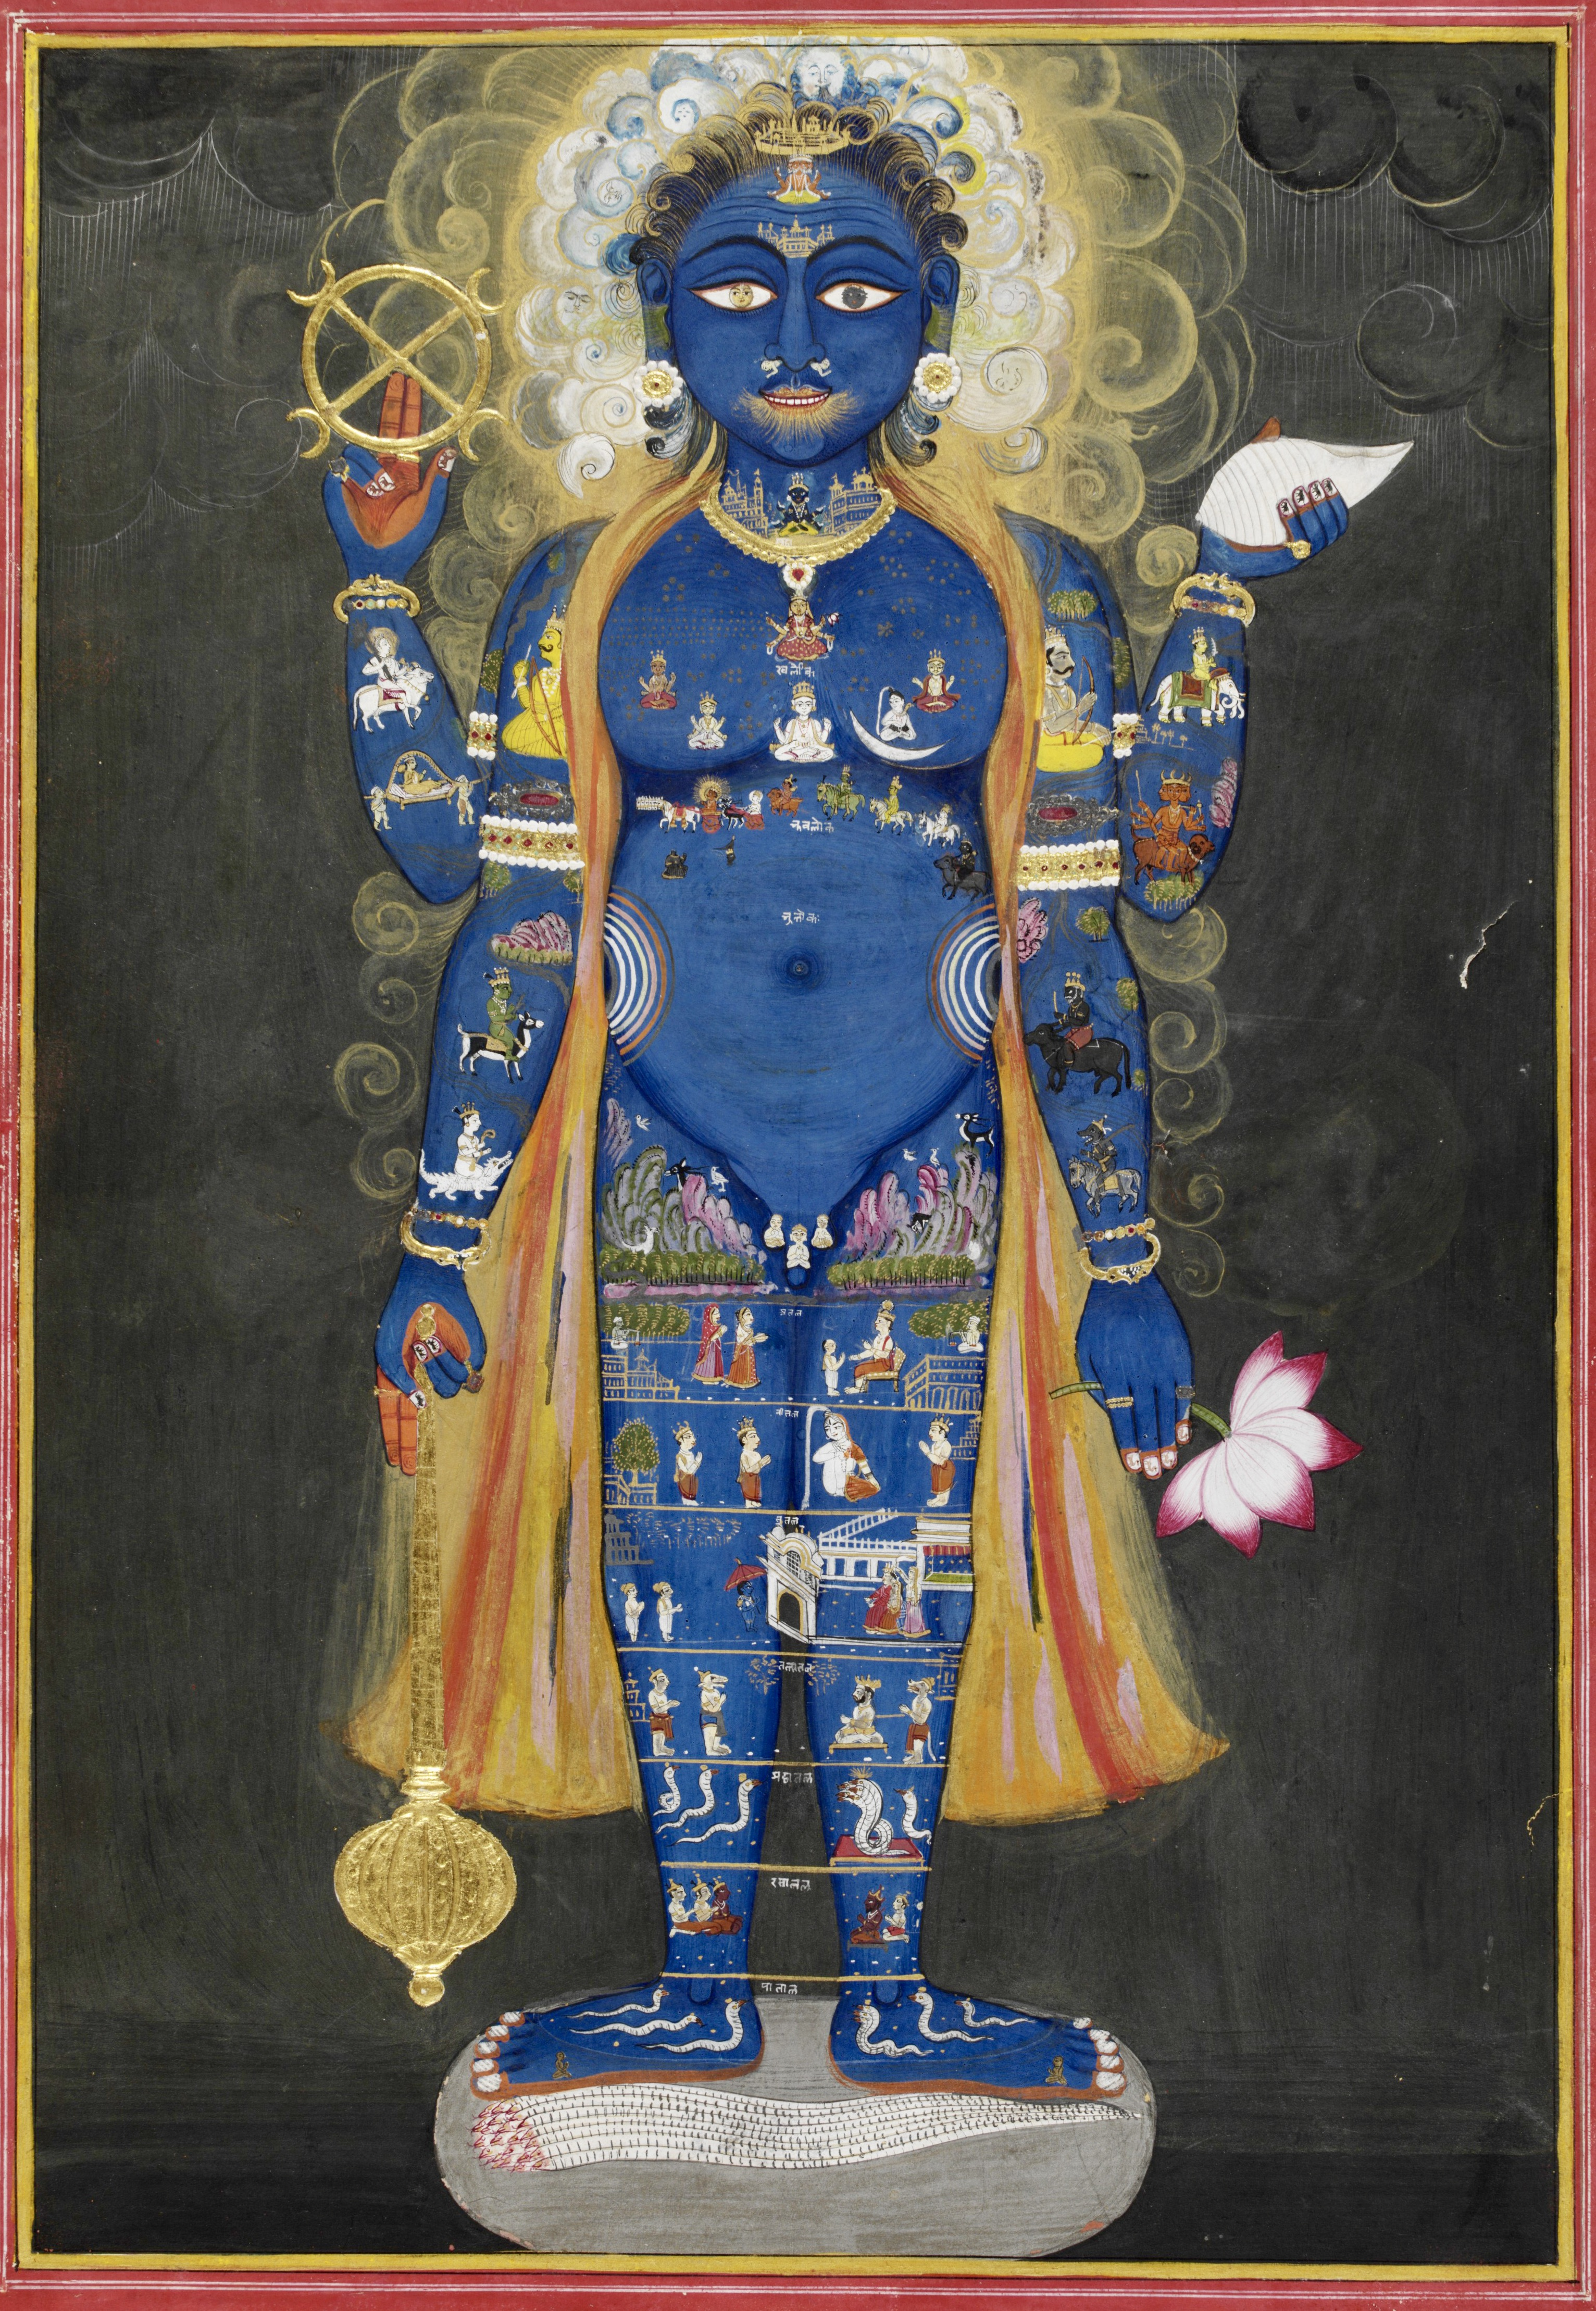
\includegraphics[width=1\textwidth]{pics/Vishnu_Vishvarupa_cropped.jpg}
	\caption{Viṣṇu Viśvarūpa, India, Rajasthan, Jaipur, ca. 1800–1820, Opaque watercolor and gold on paper, 38.5 × 28 cm, Victoria and Albert Museum, London, Given by Mrs. Gerald Clark.}
	\label{fig1}
      \end{figure}
\clearpage
  \begin{figure}[ht]
	\centering
  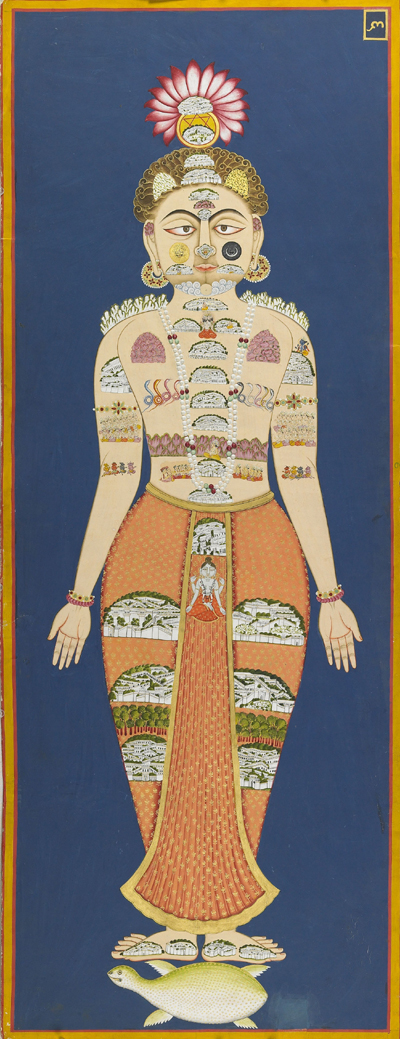
\includegraphics[width=0.5\textwidth]{pics/The_Equivalence_of_Self_and_Universe_(detail),_folio_6_from_the_Siddha_Siddhanta_Paddhati,_(Bulaki),_1824_(Samvat_1881);_122_x_46_cm._Mehrangarh_Museum_Trust..jpg}
	\caption{The Equivalence of Self and Universe (detail), folio 6 from the \textit{Siddhasiddhāntapaddhati} (Bulaki), India, Rajasthan, Jodhpur, 1824 (Samvat 1881), 122 x 46 cm, RJS 2378, Mehragarh Museum Trust.}
	\label{fig2}
      \end{figure}
      % \end{landscape}


\chapter{Bibliography}
 \label{sec:bibli}
   \clearpage
\newpage 
\thispagestyle{empty}
\quad  \addtocounter{page}{-1}

\printbibliography[heading=subbibintoc, title=Consulted Manuscripts, keyword=codex]

\printbibliography[heading=subbibintoc, title=Printed Editions, keyword=printsource]

\printbibliography[heading=subbibintoc, title=Secondary Literature, keyword=seclit]

\printbibliography[heading=subbibintoc, title=Online Sources, keyword=onlinesource]

\end{document}
